\section{Numerical Results}\label{sec:numerical-results}

In order to show that the theory holds numerically, we have devised some tests for the
non-homogeneous vector Laplace problem and the Maxwell eigenvalue problem. We focus on these
tests, which are formulated using vector fields, since the homogeneous boundary conditions
that arise in the weak formulations of these problems, both essential and natural, imply the
non-existence of harmonic scalar fields.

For all the ensuing examples, we chose to work with \(h\)-refinement for primarily two
reasons. First, it makes for more visually compelling examples of what sorts of refinements
are problematic or not. Second, using \(p\)-refinement precludes the use of maximally smooth
B-splines, which is one of the major advantages of IGA. Despite this, all the results in
\Cref{sec:exact-meshes} still hold for such refinement schemes.

\subsection{Vector Laplace problem}

Let the domain  \(\domain \subseteq \mathbb{R}^2\) be the unit square \([0,1]^2\). Since the
domain is simply connected, the continuous de Rham complex has no harmonic vector fields,
and as such, neither should our discretized complex. Considering the mixed weak formulation
of the vector Laplace problem with natural, homogeneous boundary conditions,  the relevant objects we wish to find are \(\scltrial \in
\Hone\) and \(\vectrial \in \Hcurl\) such that   
\begin{alignat*}{2}
	\langle \scltrial, \scltest\rangle - \langle \vectrial, \grad\scltest \rangle &= 0,\quad
	&&\forall \scltest \in \Hone,\\
	\langle \grad\scltrial, \vectest \rangle + \langle \curl \vectrial, \curl \vectest
	\rangle &= \langle \forcing, \vectest \rangle,\quad &&\forall \vectest\in \Hcurl.
\end{alignat*}
For the first test, we will take as the analytical solution 
\begin{equation}
    \label{eq:1-form-example-solution}
    \solution(x, y) = 
    \begin{bmatrix}
        x(1-x) \\
        0
    \end{bmatrix}.
\end{equation}
We will try to solve the problem on two different meshes ― one exact and the other not ―
just to illustrate the spurious results that can arise from  refinement that does not respect the conditions for exactness. The
two meshes are shown in \cref{fig:1-form-example}. We will denote the computed solution
using the \cref{fig:1-form-example-a,fig:1-form-example-b} meshes as \(\vectrial^a_h\) and
\(\vectrial^b_h\), respectively.
\begin{figure}[htbp]
    \centering
    \hfill
    \begin{subfigure}[b]{0.35\textwidth}
        \centering
        \input{1-form-example-a.tex}
        \caption{}
        \label{fig:1-form-example-a}
    \end{subfigure}
    \begin{subfigure}[b]{0.35\textwidth}
        \centering
        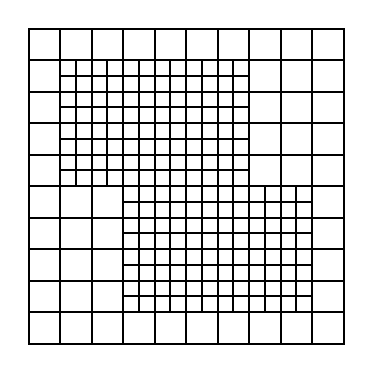
\begin{tikzpicture}[scale=4.0]
\coordinate (v1_1) at (0.0, 0.0);
\coordinate (v1_2) at (0.1, 0.0);
\coordinate (v1_3) at (0.1, 0.1);
\coordinate (v1_4) at (0.0, 0.1);
\draw[black, line width=0.75pt] (v1_1) -- (v1_2) -- (v1_3) -- (v1_4) -- cycle;
\coordinate (v2_1) at (0.1, 0.0);
\coordinate (v2_2) at (0.2, 0.0);
\coordinate (v2_3) at (0.2, 0.1);
\coordinate (v2_4) at (0.1, 0.1);
\draw[black, line width=0.75pt] (v2_1) -- (v2_2) -- (v2_3) -- (v2_4) -- cycle;
\coordinate (v3_1) at (0.2, 0.0);
\coordinate (v3_2) at (0.3, 0.0);
\coordinate (v3_3) at (0.3, 0.1);
\coordinate (v3_4) at (0.2, 0.1);
\draw[black, line width=0.75pt] (v3_1) -- (v3_2) -- (v3_3) -- (v3_4) -- cycle;
\coordinate (v4_1) at (0.3, 0.0);
\coordinate (v4_2) at (0.4, 0.0);
\coordinate (v4_3) at (0.4, 0.1);
\coordinate (v4_4) at (0.3, 0.1);
\draw[black, line width=0.75pt] (v4_1) -- (v4_2) -- (v4_3) -- (v4_4) -- cycle;
\coordinate (v5_1) at (0.4, 0.0);
\coordinate (v5_2) at (0.5, 0.0);
\coordinate (v5_3) at (0.5, 0.1);
\coordinate (v5_4) at (0.4, 0.1);
\draw[black, line width=0.75pt] (v5_1) -- (v5_2) -- (v5_3) -- (v5_4) -- cycle;
\coordinate (v6_1) at (0.5, 0.0);
\coordinate (v6_2) at (0.6, 0.0);
\coordinate (v6_3) at (0.6, 0.1);
\coordinate (v6_4) at (0.5, 0.1);
\draw[black, line width=0.75pt] (v6_1) -- (v6_2) -- (v6_3) -- (v6_4) -- cycle;
\coordinate (v7_1) at (0.6, 0.0);
\coordinate (v7_2) at (0.7, 0.0);
\coordinate (v7_3) at (0.7, 0.1);
\coordinate (v7_4) at (0.6, 0.1);
\draw[black, line width=0.75pt] (v7_1) -- (v7_2) -- (v7_3) -- (v7_4) -- cycle;
\coordinate (v8_1) at (0.7, 0.0);
\coordinate (v8_2) at (0.8, 0.0);
\coordinate (v8_3) at (0.8, 0.1);
\coordinate (v8_4) at (0.7, 0.1);
\draw[black, line width=0.75pt] (v8_1) -- (v8_2) -- (v8_3) -- (v8_4) -- cycle;
\coordinate (v9_1) at (0.8, 0.0);
\coordinate (v9_2) at (0.9, 0.0);
\coordinate (v9_3) at (0.9, 0.1);
\coordinate (v9_4) at (0.8, 0.1);
\draw[black, line width=0.75pt] (v9_1) -- (v9_2) -- (v9_3) -- (v9_4) -- cycle;
\coordinate (v10_1) at (0.9, 0.0);
\coordinate (v10_2) at (1.0, 0.0);
\coordinate (v10_3) at (1.0, 0.1);
\coordinate (v10_4) at (0.9, 0.1);
\draw[black, line width=0.75pt] (v10_1) -- (v10_2) -- (v10_3) -- (v10_4) -- cycle;
\coordinate (v11_1) at (0.0, 0.1);
\coordinate (v11_2) at (0.1, 0.1);
\coordinate (v11_3) at (0.1, 0.2);
\coordinate (v11_4) at (0.0, 0.2);
\draw[black, line width=0.75pt] (v11_1) -- (v11_2) -- (v11_3) -- (v11_4) -- cycle;
\coordinate (v12_1) at (0.1, 0.1);
\coordinate (v12_2) at (0.2, 0.1);
\coordinate (v12_3) at (0.2, 0.2);
\coordinate (v12_4) at (0.1, 0.2);
\draw[black, line width=0.75pt] (v12_1) -- (v12_2) -- (v12_3) -- (v12_4) -- cycle;
\coordinate (v13_1) at (0.2, 0.1);
\coordinate (v13_2) at (0.3, 0.1);
\coordinate (v13_3) at (0.3, 0.2);
\coordinate (v13_4) at (0.2, 0.2);
\draw[black, line width=0.75pt] (v13_1) -- (v13_2) -- (v13_3) -- (v13_4) -- cycle;
\coordinate (v14_1) at (0.9, 0.1);
\coordinate (v14_2) at (1.0, 0.1);
\coordinate (v14_3) at (1.0, 0.2);
\coordinate (v14_4) at (0.9, 0.2);
\draw[black, line width=0.75pt] (v14_1) -- (v14_2) -- (v14_3) -- (v14_4) -- cycle;
\coordinate (v15_1) at (0.0, 0.2);
\coordinate (v15_2) at (0.1, 0.2);
\coordinate (v15_3) at (0.1, 0.3);
\coordinate (v15_4) at (0.0, 0.3);
\draw[black, line width=0.75pt] (v15_1) -- (v15_2) -- (v15_3) -- (v15_4) -- cycle;
\coordinate (v16_1) at (0.1, 0.2);
\coordinate (v16_2) at (0.2, 0.2);
\coordinate (v16_3) at (0.2, 0.3);
\coordinate (v16_4) at (0.1, 0.3);
\draw[black, line width=0.75pt] (v16_1) -- (v16_2) -- (v16_3) -- (v16_4) -- cycle;
\coordinate (v17_1) at (0.2, 0.2);
\coordinate (v17_2) at (0.3, 0.2);
\coordinate (v17_3) at (0.3, 0.3);
\coordinate (v17_4) at (0.2, 0.3);
\draw[black, line width=0.75pt] (v17_1) -- (v17_2) -- (v17_3) -- (v17_4) -- cycle;
\coordinate (v18_1) at (0.9, 0.2);
\coordinate (v18_2) at (1.0, 0.2);
\coordinate (v18_3) at (1.0, 0.3);
\coordinate (v18_4) at (0.9, 0.3);
\draw[black, line width=0.75pt] (v18_1) -- (v18_2) -- (v18_3) -- (v18_4) -- cycle;
\coordinate (v19_1) at (0.0, 0.3);
\coordinate (v19_2) at (0.1, 0.3);
\coordinate (v19_3) at (0.1, 0.4);
\coordinate (v19_4) at (0.0, 0.4);
\draw[black, line width=0.75pt] (v19_1) -- (v19_2) -- (v19_3) -- (v19_4) -- cycle;
\coordinate (v20_1) at (0.1, 0.3);
\coordinate (v20_2) at (0.2, 0.3);
\coordinate (v20_3) at (0.2, 0.4);
\coordinate (v20_4) at (0.1, 0.4);
\draw[black, line width=0.75pt] (v20_1) -- (v20_2) -- (v20_3) -- (v20_4) -- cycle;
\coordinate (v21_1) at (0.2, 0.3);
\coordinate (v21_2) at (0.3, 0.3);
\coordinate (v21_3) at (0.3, 0.4);
\coordinate (v21_4) at (0.2, 0.4);
\draw[black, line width=0.75pt] (v21_1) -- (v21_2) -- (v21_3) -- (v21_4) -- cycle;
\coordinate (v22_1) at (0.9, 0.3);
\coordinate (v22_2) at (1.0, 0.3);
\coordinate (v22_3) at (1.0, 0.4);
\coordinate (v22_4) at (0.9, 0.4);
\draw[black, line width=0.75pt] (v22_1) -- (v22_2) -- (v22_3) -- (v22_4) -- cycle;
\coordinate (v23_1) at (0.0, 0.4);
\coordinate (v23_2) at (0.1, 0.4);
\coordinate (v23_3) at (0.1, 0.5);
\coordinate (v23_4) at (0.0, 0.5);
\draw[black, line width=0.75pt] (v23_1) -- (v23_2) -- (v23_3) -- (v23_4) -- cycle;
\coordinate (v24_1) at (0.1, 0.4);
\coordinate (v24_2) at (0.2, 0.4);
\coordinate (v24_3) at (0.2, 0.5);
\coordinate (v24_4) at (0.1, 0.5);
\draw[black, line width=0.75pt] (v24_1) -- (v24_2) -- (v24_3) -- (v24_4) -- cycle;
\coordinate (v25_1) at (0.2, 0.4);
\coordinate (v25_2) at (0.3, 0.4);
\coordinate (v25_3) at (0.3, 0.5);
\coordinate (v25_4) at (0.2, 0.5);
\draw[black, line width=0.75pt] (v25_1) -- (v25_2) -- (v25_3) -- (v25_4) -- cycle;
\coordinate (v26_1) at (0.9, 0.4);
\coordinate (v26_2) at (1.0, 0.4);
\coordinate (v26_3) at (1.0, 0.5);
\coordinate (v26_4) at (0.9, 0.5);
\draw[black, line width=0.75pt] (v26_1) -- (v26_2) -- (v26_3) -- (v26_4) -- cycle;
\coordinate (v27_1) at (0.0, 0.5);
\coordinate (v27_2) at (0.1, 0.5);
\coordinate (v27_3) at (0.1, 0.6);
\coordinate (v27_4) at (0.0, 0.6);
\draw[black, line width=0.75pt] (v27_1) -- (v27_2) -- (v27_3) -- (v27_4) -- cycle;
\coordinate (v28_1) at (0.7, 0.5);
\coordinate (v28_2) at (0.8, 0.5);
\coordinate (v28_3) at (0.8, 0.6);
\coordinate (v28_4) at (0.7, 0.6);
\draw[black, line width=0.75pt] (v28_1) -- (v28_2) -- (v28_3) -- (v28_4) -- cycle;
\coordinate (v29_1) at (0.8, 0.5);
\coordinate (v29_2) at (0.9, 0.5);
\coordinate (v29_3) at (0.9, 0.6);
\coordinate (v29_4) at (0.8, 0.6);
\draw[black, line width=0.75pt] (v29_1) -- (v29_2) -- (v29_3) -- (v29_4) -- cycle;
\coordinate (v30_1) at (0.9, 0.5);
\coordinate (v30_2) at (1.0, 0.5);
\coordinate (v30_3) at (1.0, 0.6);
\coordinate (v30_4) at (0.9, 0.6);
\draw[black, line width=0.75pt] (v30_1) -- (v30_2) -- (v30_3) -- (v30_4) -- cycle;
\coordinate (v31_1) at (0.0, 0.6);
\coordinate (v31_2) at (0.1, 0.6);
\coordinate (v31_3) at (0.1, 0.7);
\coordinate (v31_4) at (0.0, 0.7);
\draw[black, line width=0.75pt] (v31_1) -- (v31_2) -- (v31_3) -- (v31_4) -- cycle;
\coordinate (v32_1) at (0.7, 0.6);
\coordinate (v32_2) at (0.8, 0.6);
\coordinate (v32_3) at (0.8, 0.7);
\coordinate (v32_4) at (0.7, 0.7);
\draw[black, line width=0.75pt] (v32_1) -- (v32_2) -- (v32_3) -- (v32_4) -- cycle;
\coordinate (v33_1) at (0.8, 0.6);
\coordinate (v33_2) at (0.9, 0.6);
\coordinate (v33_3) at (0.9, 0.7);
\coordinate (v33_4) at (0.8, 0.7);
\draw[black, line width=0.75pt] (v33_1) -- (v33_2) -- (v33_3) -- (v33_4) -- cycle;
\coordinate (v34_1) at (0.9, 0.6);
\coordinate (v34_2) at (1.0, 0.6);
\coordinate (v34_3) at (1.0, 0.7);
\coordinate (v34_4) at (0.9, 0.7);
\draw[black, line width=0.75pt] (v34_1) -- (v34_2) -- (v34_3) -- (v34_4) -- cycle;
\coordinate (v35_1) at (0.0, 0.7);
\coordinate (v35_2) at (0.1, 0.7);
\coordinate (v35_3) at (0.1, 0.8);
\coordinate (v35_4) at (0.0, 0.8);
\draw[black, line width=0.75pt] (v35_1) -- (v35_2) -- (v35_3) -- (v35_4) -- cycle;
\coordinate (v36_1) at (0.7, 0.7);
\coordinate (v36_2) at (0.8, 0.7);
\coordinate (v36_3) at (0.8, 0.8);
\coordinate (v36_4) at (0.7, 0.8);
\draw[black, line width=0.75pt] (v36_1) -- (v36_2) -- (v36_3) -- (v36_4) -- cycle;
\coordinate (v37_1) at (0.8, 0.7);
\coordinate (v37_2) at (0.9, 0.7);
\coordinate (v37_3) at (0.9, 0.8);
\coordinate (v37_4) at (0.8, 0.8);
\draw[black, line width=0.75pt] (v37_1) -- (v37_2) -- (v37_3) -- (v37_4) -- cycle;
\coordinate (v38_1) at (0.9, 0.7);
\coordinate (v38_2) at (1.0, 0.7);
\coordinate (v38_3) at (1.0, 0.8);
\coordinate (v38_4) at (0.9, 0.8);
\draw[black, line width=0.75pt] (v38_1) -- (v38_2) -- (v38_3) -- (v38_4) -- cycle;
\coordinate (v39_1) at (0.0, 0.8);
\coordinate (v39_2) at (0.1, 0.8);
\coordinate (v39_3) at (0.1, 0.9);
\coordinate (v39_4) at (0.0, 0.9);
\draw[black, line width=0.75pt] (v39_1) -- (v39_2) -- (v39_3) -- (v39_4) -- cycle;
\coordinate (v40_1) at (0.7, 0.8);
\coordinate (v40_2) at (0.8, 0.8);
\coordinate (v40_3) at (0.8, 0.9);
\coordinate (v40_4) at (0.7, 0.9);
\draw[black, line width=0.75pt] (v40_1) -- (v40_2) -- (v40_3) -- (v40_4) -- cycle;
\coordinate (v41_1) at (0.8, 0.8);
\coordinate (v41_2) at (0.9, 0.8);
\coordinate (v41_3) at (0.9, 0.9);
\coordinate (v41_4) at (0.8, 0.9);
\draw[black, line width=0.75pt] (v41_1) -- (v41_2) -- (v41_3) -- (v41_4) -- cycle;
\coordinate (v42_1) at (0.9, 0.8);
\coordinate (v42_2) at (1.0, 0.8);
\coordinate (v42_3) at (1.0, 0.9);
\coordinate (v42_4) at (0.9, 0.9);
\draw[black, line width=0.75pt] (v42_1) -- (v42_2) -- (v42_3) -- (v42_4) -- cycle;
\coordinate (v43_1) at (0.0, 0.9);
\coordinate (v43_2) at (0.1, 0.9);
\coordinate (v43_3) at (0.1, 1.0);
\coordinate (v43_4) at (0.0, 1.0);
\draw[black, line width=0.75pt] (v43_1) -- (v43_2) -- (v43_3) -- (v43_4) -- cycle;
\coordinate (v44_1) at (0.1, 0.9);
\coordinate (v44_2) at (0.2, 0.9);
\coordinate (v44_3) at (0.2, 1.0);
\coordinate (v44_4) at (0.1, 1.0);
\draw[black, line width=0.75pt] (v44_1) -- (v44_2) -- (v44_3) -- (v44_4) -- cycle;
\coordinate (v45_1) at (0.2, 0.9);
\coordinate (v45_2) at (0.3, 0.9);
\coordinate (v45_3) at (0.3, 1.0);
\coordinate (v45_4) at (0.2, 1.0);
\draw[black, line width=0.75pt] (v45_1) -- (v45_2) -- (v45_3) -- (v45_4) -- cycle;
\coordinate (v46_1) at (0.3, 0.9);
\coordinate (v46_2) at (0.4, 0.9);
\coordinate (v46_3) at (0.4, 1.0);
\coordinate (v46_4) at (0.3, 1.0);
\draw[black, line width=0.75pt] (v46_1) -- (v46_2) -- (v46_3) -- (v46_4) -- cycle;
\coordinate (v47_1) at (0.4, 0.9);
\coordinate (v47_2) at (0.5, 0.9);
\coordinate (v47_3) at (0.5, 1.0);
\coordinate (v47_4) at (0.4, 1.0);
\draw[black, line width=0.75pt] (v47_1) -- (v47_2) -- (v47_3) -- (v47_4) -- cycle;
\coordinate (v48_1) at (0.5, 0.9);
\coordinate (v48_2) at (0.6, 0.9);
\coordinate (v48_3) at (0.6, 1.0);
\coordinate (v48_4) at (0.5, 1.0);
\draw[black, line width=0.75pt] (v48_1) -- (v48_2) -- (v48_3) -- (v48_4) -- cycle;
\coordinate (v49_1) at (0.6, 0.9);
\coordinate (v49_2) at (0.7, 0.9);
\coordinate (v49_3) at (0.7, 1.0);
\coordinate (v49_4) at (0.6, 1.0);
\draw[black, line width=0.75pt] (v49_1) -- (v49_2) -- (v49_3) -- (v49_4) -- cycle;
\coordinate (v50_1) at (0.7, 0.9);
\coordinate (v50_2) at (0.8, 0.9);
\coordinate (v50_3) at (0.8, 1.0);
\coordinate (v50_4) at (0.7, 1.0);
\draw[black, line width=0.75pt] (v50_1) -- (v50_2) -- (v50_3) -- (v50_4) -- cycle;
\coordinate (v51_1) at (0.8, 0.9);
\coordinate (v51_2) at (0.9, 0.9);
\coordinate (v51_3) at (0.9, 1.0);
\coordinate (v51_4) at (0.8, 1.0);
\draw[black, line width=0.75pt] (v51_1) -- (v51_2) -- (v51_3) -- (v51_4) -- cycle;
\coordinate (v52_1) at (0.9, 0.9);
\coordinate (v52_2) at (1.0, 0.9);
\coordinate (v52_3) at (1.0, 1.0);
\coordinate (v52_4) at (0.9, 1.0);
\draw[black, line width=0.75pt] (v52_1) -- (v52_2) -- (v52_3) -- (v52_4) -- cycle;
\coordinate (v53_1) at (0.3, 0.1);
\coordinate (v53_2) at (0.35, 0.1);
\coordinate (v53_3) at (0.35, 0.15000000000000002);
\coordinate (v53_4) at (0.3, 0.15000000000000002);
\draw[black, line width=0.75pt] (v53_1) -- (v53_2) -- (v53_3) -- (v53_4) -- cycle;
\coordinate (v54_1) at (0.35, 0.1);
\coordinate (v54_2) at (0.4, 0.1);
\coordinate (v54_3) at (0.4, 0.15000000000000002);
\coordinate (v54_4) at (0.35, 0.15000000000000002);
\draw[black, line width=0.75pt] (v54_1) -- (v54_2) -- (v54_3) -- (v54_4) -- cycle;
\coordinate (v55_1) at (0.4, 0.1);
\coordinate (v55_2) at (0.45, 0.1);
\coordinate (v55_3) at (0.45, 0.15000000000000002);
\coordinate (v55_4) at (0.4, 0.15000000000000002);
\draw[black, line width=0.75pt] (v55_1) -- (v55_2) -- (v55_3) -- (v55_4) -- cycle;
\coordinate (v56_1) at (0.45, 0.1);
\coordinate (v56_2) at (0.5, 0.1);
\coordinate (v56_3) at (0.5, 0.15000000000000002);
\coordinate (v56_4) at (0.45, 0.15000000000000002);
\draw[black, line width=0.75pt] (v56_1) -- (v56_2) -- (v56_3) -- (v56_4) -- cycle;
\coordinate (v57_1) at (0.5, 0.1);
\coordinate (v57_2) at (0.55, 0.1);
\coordinate (v57_3) at (0.55, 0.15000000000000002);
\coordinate (v57_4) at (0.5, 0.15000000000000002);
\draw[black, line width=0.75pt] (v57_1) -- (v57_2) -- (v57_3) -- (v57_4) -- cycle;
\coordinate (v58_1) at (0.55, 0.1);
\coordinate (v58_2) at (0.6, 0.1);
\coordinate (v58_3) at (0.6, 0.15000000000000002);
\coordinate (v58_4) at (0.55, 0.15000000000000002);
\draw[black, line width=0.75pt] (v58_1) -- (v58_2) -- (v58_3) -- (v58_4) -- cycle;
\coordinate (v59_1) at (0.6, 0.1);
\coordinate (v59_2) at (0.6499999999999999, 0.1);
\coordinate (v59_3) at (0.6499999999999999, 0.15000000000000002);
\coordinate (v59_4) at (0.6, 0.15000000000000002);
\draw[black, line width=0.75pt] (v59_1) -- (v59_2) -- (v59_3) -- (v59_4) -- cycle;
\coordinate (v60_1) at (0.6499999999999999, 0.1);
\coordinate (v60_2) at (0.7, 0.1);
\coordinate (v60_3) at (0.7, 0.15000000000000002);
\coordinate (v60_4) at (0.6499999999999999, 0.15000000000000002);
\draw[black, line width=0.75pt] (v60_1) -- (v60_2) -- (v60_3) -- (v60_4) -- cycle;
\coordinate (v61_1) at (0.7, 0.1);
\coordinate (v61_2) at (0.75, 0.1);
\coordinate (v61_3) at (0.75, 0.15000000000000002);
\coordinate (v61_4) at (0.7, 0.15000000000000002);
\draw[black, line width=0.75pt] (v61_1) -- (v61_2) -- (v61_3) -- (v61_4) -- cycle;
\coordinate (v62_1) at (0.75, 0.1);
\coordinate (v62_2) at (0.8, 0.1);
\coordinate (v62_3) at (0.8, 0.15000000000000002);
\coordinate (v62_4) at (0.75, 0.15000000000000002);
\draw[black, line width=0.75pt] (v62_1) -- (v62_2) -- (v62_3) -- (v62_4) -- cycle;
\coordinate (v63_1) at (0.8, 0.1);
\coordinate (v63_2) at (0.8500000000000001, 0.1);
\coordinate (v63_3) at (0.8500000000000001, 0.15000000000000002);
\coordinate (v63_4) at (0.8, 0.15000000000000002);
\draw[black, line width=0.75pt] (v63_1) -- (v63_2) -- (v63_3) -- (v63_4) -- cycle;
\coordinate (v64_1) at (0.8500000000000001, 0.1);
\coordinate (v64_2) at (0.9, 0.1);
\coordinate (v64_3) at (0.9, 0.15000000000000002);
\coordinate (v64_4) at (0.8500000000000001, 0.15000000000000002);
\draw[black, line width=0.75pt] (v64_1) -- (v64_2) -- (v64_3) -- (v64_4) -- cycle;
\coordinate (v65_1) at (0.3, 0.15000000000000002);
\coordinate (v65_2) at (0.35, 0.15000000000000002);
\coordinate (v65_3) at (0.35, 0.2);
\coordinate (v65_4) at (0.3, 0.2);
\draw[black, line width=0.75pt] (v65_1) -- (v65_2) -- (v65_3) -- (v65_4) -- cycle;
\coordinate (v66_1) at (0.35, 0.15000000000000002);
\coordinate (v66_2) at (0.4, 0.15000000000000002);
\coordinate (v66_3) at (0.4, 0.2);
\coordinate (v66_4) at (0.35, 0.2);
\draw[black, line width=0.75pt] (v66_1) -- (v66_2) -- (v66_3) -- (v66_4) -- cycle;
\coordinate (v67_1) at (0.4, 0.15000000000000002);
\coordinate (v67_2) at (0.45, 0.15000000000000002);
\coordinate (v67_3) at (0.45, 0.2);
\coordinate (v67_4) at (0.4, 0.2);
\draw[black, line width=0.75pt] (v67_1) -- (v67_2) -- (v67_3) -- (v67_4) -- cycle;
\coordinate (v68_1) at (0.45, 0.15000000000000002);
\coordinate (v68_2) at (0.5, 0.15000000000000002);
\coordinate (v68_3) at (0.5, 0.2);
\coordinate (v68_4) at (0.45, 0.2);
\draw[black, line width=0.75pt] (v68_1) -- (v68_2) -- (v68_3) -- (v68_4) -- cycle;
\coordinate (v69_1) at (0.5, 0.15000000000000002);
\coordinate (v69_2) at (0.55, 0.15000000000000002);
\coordinate (v69_3) at (0.55, 0.2);
\coordinate (v69_4) at (0.5, 0.2);
\draw[black, line width=0.75pt] (v69_1) -- (v69_2) -- (v69_3) -- (v69_4) -- cycle;
\coordinate (v70_1) at (0.55, 0.15000000000000002);
\coordinate (v70_2) at (0.6, 0.15000000000000002);
\coordinate (v70_3) at (0.6, 0.2);
\coordinate (v70_4) at (0.55, 0.2);
\draw[black, line width=0.75pt] (v70_1) -- (v70_2) -- (v70_3) -- (v70_4) -- cycle;
\coordinate (v71_1) at (0.6, 0.15000000000000002);
\coordinate (v71_2) at (0.6499999999999999, 0.15000000000000002);
\coordinate (v71_3) at (0.6499999999999999, 0.2);
\coordinate (v71_4) at (0.6, 0.2);
\draw[black, line width=0.75pt] (v71_1) -- (v71_2) -- (v71_3) -- (v71_4) -- cycle;
\coordinate (v72_1) at (0.6499999999999999, 0.15000000000000002);
\coordinate (v72_2) at (0.7, 0.15000000000000002);
\coordinate (v72_3) at (0.7, 0.2);
\coordinate (v72_4) at (0.6499999999999999, 0.2);
\draw[black, line width=0.75pt] (v72_1) -- (v72_2) -- (v72_3) -- (v72_4) -- cycle;
\coordinate (v73_1) at (0.7, 0.15000000000000002);
\coordinate (v73_2) at (0.75, 0.15000000000000002);
\coordinate (v73_3) at (0.75, 0.2);
\coordinate (v73_4) at (0.7, 0.2);
\draw[black, line width=0.75pt] (v73_1) -- (v73_2) -- (v73_3) -- (v73_4) -- cycle;
\coordinate (v74_1) at (0.75, 0.15000000000000002);
\coordinate (v74_2) at (0.8, 0.15000000000000002);
\coordinate (v74_3) at (0.8, 0.2);
\coordinate (v74_4) at (0.75, 0.2);
\draw[black, line width=0.75pt] (v74_1) -- (v74_2) -- (v74_3) -- (v74_4) -- cycle;
\coordinate (v75_1) at (0.8, 0.15000000000000002);
\coordinate (v75_2) at (0.8500000000000001, 0.15000000000000002);
\coordinate (v75_3) at (0.8500000000000001, 0.2);
\coordinate (v75_4) at (0.8, 0.2);
\draw[black, line width=0.75pt] (v75_1) -- (v75_2) -- (v75_3) -- (v75_4) -- cycle;
\coordinate (v76_1) at (0.8500000000000001, 0.15000000000000002);
\coordinate (v76_2) at (0.9, 0.15000000000000002);
\coordinate (v76_3) at (0.9, 0.2);
\coordinate (v76_4) at (0.8500000000000001, 0.2);
\draw[black, line width=0.75pt] (v76_1) -- (v76_2) -- (v76_3) -- (v76_4) -- cycle;
\coordinate (v77_1) at (0.3, 0.2);
\coordinate (v77_2) at (0.35, 0.2);
\coordinate (v77_3) at (0.35, 0.25);
\coordinate (v77_4) at (0.3, 0.25);
\draw[black, line width=0.75pt] (v77_1) -- (v77_2) -- (v77_3) -- (v77_4) -- cycle;
\coordinate (v78_1) at (0.35, 0.2);
\coordinate (v78_2) at (0.4, 0.2);
\coordinate (v78_3) at (0.4, 0.25);
\coordinate (v78_4) at (0.35, 0.25);
\draw[black, line width=0.75pt] (v78_1) -- (v78_2) -- (v78_3) -- (v78_4) -- cycle;
\coordinate (v79_1) at (0.4, 0.2);
\coordinate (v79_2) at (0.45, 0.2);
\coordinate (v79_3) at (0.45, 0.25);
\coordinate (v79_4) at (0.4, 0.25);
\draw[black, line width=0.75pt] (v79_1) -- (v79_2) -- (v79_3) -- (v79_4) -- cycle;
\coordinate (v80_1) at (0.45, 0.2);
\coordinate (v80_2) at (0.5, 0.2);
\coordinate (v80_3) at (0.5, 0.25);
\coordinate (v80_4) at (0.45, 0.25);
\draw[black, line width=0.75pt] (v80_1) -- (v80_2) -- (v80_3) -- (v80_4) -- cycle;
\coordinate (v81_1) at (0.5, 0.2);
\coordinate (v81_2) at (0.55, 0.2);
\coordinate (v81_3) at (0.55, 0.25);
\coordinate (v81_4) at (0.5, 0.25);
\draw[black, line width=0.75pt] (v81_1) -- (v81_2) -- (v81_3) -- (v81_4) -- cycle;
\coordinate (v82_1) at (0.55, 0.2);
\coordinate (v82_2) at (0.6, 0.2);
\coordinate (v82_3) at (0.6, 0.25);
\coordinate (v82_4) at (0.55, 0.25);
\draw[black, line width=0.75pt] (v82_1) -- (v82_2) -- (v82_3) -- (v82_4) -- cycle;
\coordinate (v83_1) at (0.6, 0.2);
\coordinate (v83_2) at (0.6499999999999999, 0.2);
\coordinate (v83_3) at (0.6499999999999999, 0.25);
\coordinate (v83_4) at (0.6, 0.25);
\draw[black, line width=0.75pt] (v83_1) -- (v83_2) -- (v83_3) -- (v83_4) -- cycle;
\coordinate (v84_1) at (0.6499999999999999, 0.2);
\coordinate (v84_2) at (0.7, 0.2);
\coordinate (v84_3) at (0.7, 0.25);
\coordinate (v84_4) at (0.6499999999999999, 0.25);
\draw[black, line width=0.75pt] (v84_1) -- (v84_2) -- (v84_3) -- (v84_4) -- cycle;
\coordinate (v85_1) at (0.7, 0.2);
\coordinate (v85_2) at (0.75, 0.2);
\coordinate (v85_3) at (0.75, 0.25);
\coordinate (v85_4) at (0.7, 0.25);
\draw[black, line width=0.75pt] (v85_1) -- (v85_2) -- (v85_3) -- (v85_4) -- cycle;
\coordinate (v86_1) at (0.75, 0.2);
\coordinate (v86_2) at (0.8, 0.2);
\coordinate (v86_3) at (0.8, 0.25);
\coordinate (v86_4) at (0.75, 0.25);
\draw[black, line width=0.75pt] (v86_1) -- (v86_2) -- (v86_3) -- (v86_4) -- cycle;
\coordinate (v87_1) at (0.8, 0.2);
\coordinate (v87_2) at (0.8500000000000001, 0.2);
\coordinate (v87_3) at (0.8500000000000001, 0.25);
\coordinate (v87_4) at (0.8, 0.25);
\draw[black, line width=0.75pt] (v87_1) -- (v87_2) -- (v87_3) -- (v87_4) -- cycle;
\coordinate (v88_1) at (0.8500000000000001, 0.2);
\coordinate (v88_2) at (0.9, 0.2);
\coordinate (v88_3) at (0.9, 0.25);
\coordinate (v88_4) at (0.8500000000000001, 0.25);
\draw[black, line width=0.75pt] (v88_1) -- (v88_2) -- (v88_3) -- (v88_4) -- cycle;
\coordinate (v89_1) at (0.3, 0.25);
\coordinate (v89_2) at (0.35, 0.25);
\coordinate (v89_3) at (0.35, 0.3);
\coordinate (v89_4) at (0.3, 0.3);
\draw[black, line width=0.75pt] (v89_1) -- (v89_2) -- (v89_3) -- (v89_4) -- cycle;
\coordinate (v90_1) at (0.35, 0.25);
\coordinate (v90_2) at (0.4, 0.25);
\coordinate (v90_3) at (0.4, 0.3);
\coordinate (v90_4) at (0.35, 0.3);
\draw[black, line width=0.75pt] (v90_1) -- (v90_2) -- (v90_3) -- (v90_4) -- cycle;
\coordinate (v91_1) at (0.4, 0.25);
\coordinate (v91_2) at (0.45, 0.25);
\coordinate (v91_3) at (0.45, 0.3);
\coordinate (v91_4) at (0.4, 0.3);
\draw[black, line width=0.75pt] (v91_1) -- (v91_2) -- (v91_3) -- (v91_4) -- cycle;
\coordinate (v92_1) at (0.45, 0.25);
\coordinate (v92_2) at (0.5, 0.25);
\coordinate (v92_3) at (0.5, 0.3);
\coordinate (v92_4) at (0.45, 0.3);
\draw[black, line width=0.75pt] (v92_1) -- (v92_2) -- (v92_3) -- (v92_4) -- cycle;
\coordinate (v93_1) at (0.5, 0.25);
\coordinate (v93_2) at (0.55, 0.25);
\coordinate (v93_3) at (0.55, 0.3);
\coordinate (v93_4) at (0.5, 0.3);
\draw[black, line width=0.75pt] (v93_1) -- (v93_2) -- (v93_3) -- (v93_4) -- cycle;
\coordinate (v94_1) at (0.55, 0.25);
\coordinate (v94_2) at (0.6, 0.25);
\coordinate (v94_3) at (0.6, 0.3);
\coordinate (v94_4) at (0.55, 0.3);
\draw[black, line width=0.75pt] (v94_1) -- (v94_2) -- (v94_3) -- (v94_4) -- cycle;
\coordinate (v95_1) at (0.6, 0.25);
\coordinate (v95_2) at (0.6499999999999999, 0.25);
\coordinate (v95_3) at (0.6499999999999999, 0.3);
\coordinate (v95_4) at (0.6, 0.3);
\draw[black, line width=0.75pt] (v95_1) -- (v95_2) -- (v95_3) -- (v95_4) -- cycle;
\coordinate (v96_1) at (0.6499999999999999, 0.25);
\coordinate (v96_2) at (0.7, 0.25);
\coordinate (v96_3) at (0.7, 0.3);
\coordinate (v96_4) at (0.6499999999999999, 0.3);
\draw[black, line width=0.75pt] (v96_1) -- (v96_2) -- (v96_3) -- (v96_4) -- cycle;
\coordinate (v97_1) at (0.7, 0.25);
\coordinate (v97_2) at (0.75, 0.25);
\coordinate (v97_3) at (0.75, 0.3);
\coordinate (v97_4) at (0.7, 0.3);
\draw[black, line width=0.75pt] (v97_1) -- (v97_2) -- (v97_3) -- (v97_4) -- cycle;
\coordinate (v98_1) at (0.75, 0.25);
\coordinate (v98_2) at (0.8, 0.25);
\coordinate (v98_3) at (0.8, 0.3);
\coordinate (v98_4) at (0.75, 0.3);
\draw[black, line width=0.75pt] (v98_1) -- (v98_2) -- (v98_3) -- (v98_4) -- cycle;
\coordinate (v99_1) at (0.8, 0.25);
\coordinate (v99_2) at (0.8500000000000001, 0.25);
\coordinate (v99_3) at (0.8500000000000001, 0.3);
\coordinate (v99_4) at (0.8, 0.3);
\draw[black, line width=0.75pt] (v99_1) -- (v99_2) -- (v99_3) -- (v99_4) -- cycle;
\coordinate (v100_1) at (0.8500000000000001, 0.25);
\coordinate (v100_2) at (0.9, 0.25);
\coordinate (v100_3) at (0.9, 0.3);
\coordinate (v100_4) at (0.8500000000000001, 0.3);
\draw[black, line width=0.75pt] (v100_1) -- (v100_2) -- (v100_3) -- (v100_4) -- cycle;
\coordinate (v101_1) at (0.3, 0.3);
\coordinate (v101_2) at (0.35, 0.3);
\coordinate (v101_3) at (0.35, 0.35);
\coordinate (v101_4) at (0.3, 0.35);
\draw[black, line width=0.75pt] (v101_1) -- (v101_2) -- (v101_3) -- (v101_4) -- cycle;
\coordinate (v102_1) at (0.35, 0.3);
\coordinate (v102_2) at (0.4, 0.3);
\coordinate (v102_3) at (0.4, 0.35);
\coordinate (v102_4) at (0.35, 0.35);
\draw[black, line width=0.75pt] (v102_1) -- (v102_2) -- (v102_3) -- (v102_4) -- cycle;
\coordinate (v103_1) at (0.4, 0.3);
\coordinate (v103_2) at (0.45, 0.3);
\coordinate (v103_3) at (0.45, 0.35);
\coordinate (v103_4) at (0.4, 0.35);
\draw[black, line width=0.75pt] (v103_1) -- (v103_2) -- (v103_3) -- (v103_4) -- cycle;
\coordinate (v104_1) at (0.45, 0.3);
\coordinate (v104_2) at (0.5, 0.3);
\coordinate (v104_3) at (0.5, 0.35);
\coordinate (v104_4) at (0.45, 0.35);
\draw[black, line width=0.75pt] (v104_1) -- (v104_2) -- (v104_3) -- (v104_4) -- cycle;
\coordinate (v105_1) at (0.5, 0.3);
\coordinate (v105_2) at (0.55, 0.3);
\coordinate (v105_3) at (0.55, 0.35);
\coordinate (v105_4) at (0.5, 0.35);
\draw[black, line width=0.75pt] (v105_1) -- (v105_2) -- (v105_3) -- (v105_4) -- cycle;
\coordinate (v106_1) at (0.55, 0.3);
\coordinate (v106_2) at (0.6, 0.3);
\coordinate (v106_3) at (0.6, 0.35);
\coordinate (v106_4) at (0.55, 0.35);
\draw[black, line width=0.75pt] (v106_1) -- (v106_2) -- (v106_3) -- (v106_4) -- cycle;
\coordinate (v107_1) at (0.6, 0.3);
\coordinate (v107_2) at (0.6499999999999999, 0.3);
\coordinate (v107_3) at (0.6499999999999999, 0.35);
\coordinate (v107_4) at (0.6, 0.35);
\draw[black, line width=0.75pt] (v107_1) -- (v107_2) -- (v107_3) -- (v107_4) -- cycle;
\coordinate (v108_1) at (0.6499999999999999, 0.3);
\coordinate (v108_2) at (0.7, 0.3);
\coordinate (v108_3) at (0.7, 0.35);
\coordinate (v108_4) at (0.6499999999999999, 0.35);
\draw[black, line width=0.75pt] (v108_1) -- (v108_2) -- (v108_3) -- (v108_4) -- cycle;
\coordinate (v109_1) at (0.7, 0.3);
\coordinate (v109_2) at (0.75, 0.3);
\coordinate (v109_3) at (0.75, 0.35);
\coordinate (v109_4) at (0.7, 0.35);
\draw[black, line width=0.75pt] (v109_1) -- (v109_2) -- (v109_3) -- (v109_4) -- cycle;
\coordinate (v110_1) at (0.75, 0.3);
\coordinate (v110_2) at (0.8, 0.3);
\coordinate (v110_3) at (0.8, 0.35);
\coordinate (v110_4) at (0.75, 0.35);
\draw[black, line width=0.75pt] (v110_1) -- (v110_2) -- (v110_3) -- (v110_4) -- cycle;
\coordinate (v111_1) at (0.8, 0.3);
\coordinate (v111_2) at (0.8500000000000001, 0.3);
\coordinate (v111_3) at (0.8500000000000001, 0.35);
\coordinate (v111_4) at (0.8, 0.35);
\draw[black, line width=0.75pt] (v111_1) -- (v111_2) -- (v111_3) -- (v111_4) -- cycle;
\coordinate (v112_1) at (0.8500000000000001, 0.3);
\coordinate (v112_2) at (0.9, 0.3);
\coordinate (v112_3) at (0.9, 0.35);
\coordinate (v112_4) at (0.8500000000000001, 0.35);
\draw[black, line width=0.75pt] (v112_1) -- (v112_2) -- (v112_3) -- (v112_4) -- cycle;
\coordinate (v113_1) at (0.3, 0.35);
\coordinate (v113_2) at (0.35, 0.35);
\coordinate (v113_3) at (0.35, 0.4);
\coordinate (v113_4) at (0.3, 0.4);
\draw[black, line width=0.75pt] (v113_1) -- (v113_2) -- (v113_3) -- (v113_4) -- cycle;
\coordinate (v114_1) at (0.35, 0.35);
\coordinate (v114_2) at (0.4, 0.35);
\coordinate (v114_3) at (0.4, 0.4);
\coordinate (v114_4) at (0.35, 0.4);
\draw[black, line width=0.75pt] (v114_1) -- (v114_2) -- (v114_3) -- (v114_4) -- cycle;
\coordinate (v115_1) at (0.4, 0.35);
\coordinate (v115_2) at (0.45, 0.35);
\coordinate (v115_3) at (0.45, 0.4);
\coordinate (v115_4) at (0.4, 0.4);
\draw[black, line width=0.75pt] (v115_1) -- (v115_2) -- (v115_3) -- (v115_4) -- cycle;
\coordinate (v116_1) at (0.45, 0.35);
\coordinate (v116_2) at (0.5, 0.35);
\coordinate (v116_3) at (0.5, 0.4);
\coordinate (v116_4) at (0.45, 0.4);
\draw[black, line width=0.75pt] (v116_1) -- (v116_2) -- (v116_3) -- (v116_4) -- cycle;
\coordinate (v117_1) at (0.5, 0.35);
\coordinate (v117_2) at (0.55, 0.35);
\coordinate (v117_3) at (0.55, 0.4);
\coordinate (v117_4) at (0.5, 0.4);
\draw[black, line width=0.75pt] (v117_1) -- (v117_2) -- (v117_3) -- (v117_4) -- cycle;
\coordinate (v118_1) at (0.55, 0.35);
\coordinate (v118_2) at (0.6, 0.35);
\coordinate (v118_3) at (0.6, 0.4);
\coordinate (v118_4) at (0.55, 0.4);
\draw[black, line width=0.75pt] (v118_1) -- (v118_2) -- (v118_3) -- (v118_4) -- cycle;
\coordinate (v119_1) at (0.6, 0.35);
\coordinate (v119_2) at (0.6499999999999999, 0.35);
\coordinate (v119_3) at (0.6499999999999999, 0.4);
\coordinate (v119_4) at (0.6, 0.4);
\draw[black, line width=0.75pt] (v119_1) -- (v119_2) -- (v119_3) -- (v119_4) -- cycle;
\coordinate (v120_1) at (0.6499999999999999, 0.35);
\coordinate (v120_2) at (0.7, 0.35);
\coordinate (v120_3) at (0.7, 0.4);
\coordinate (v120_4) at (0.6499999999999999, 0.4);
\draw[black, line width=0.75pt] (v120_1) -- (v120_2) -- (v120_3) -- (v120_4) -- cycle;
\coordinate (v121_1) at (0.7, 0.35);
\coordinate (v121_2) at (0.75, 0.35);
\coordinate (v121_3) at (0.75, 0.4);
\coordinate (v121_4) at (0.7, 0.4);
\draw[black, line width=0.75pt] (v121_1) -- (v121_2) -- (v121_3) -- (v121_4) -- cycle;
\coordinate (v122_1) at (0.75, 0.35);
\coordinate (v122_2) at (0.8, 0.35);
\coordinate (v122_3) at (0.8, 0.4);
\coordinate (v122_4) at (0.75, 0.4);
\draw[black, line width=0.75pt] (v122_1) -- (v122_2) -- (v122_3) -- (v122_4) -- cycle;
\coordinate (v123_1) at (0.8, 0.35);
\coordinate (v123_2) at (0.8500000000000001, 0.35);
\coordinate (v123_3) at (0.8500000000000001, 0.4);
\coordinate (v123_4) at (0.8, 0.4);
\draw[black, line width=0.75pt] (v123_1) -- (v123_2) -- (v123_3) -- (v123_4) -- cycle;
\coordinate (v124_1) at (0.8500000000000001, 0.35);
\coordinate (v124_2) at (0.9, 0.35);
\coordinate (v124_3) at (0.9, 0.4);
\coordinate (v124_4) at (0.8500000000000001, 0.4);
\draw[black, line width=0.75pt] (v124_1) -- (v124_2) -- (v124_3) -- (v124_4) -- cycle;
\coordinate (v125_1) at (0.3, 0.4);
\coordinate (v125_2) at (0.35, 0.4);
\coordinate (v125_3) at (0.35, 0.45);
\coordinate (v125_4) at (0.3, 0.45);
\draw[black, line width=0.75pt] (v125_1) -- (v125_2) -- (v125_3) -- (v125_4) -- cycle;
\coordinate (v126_1) at (0.35, 0.4);
\coordinate (v126_2) at (0.4, 0.4);
\coordinate (v126_3) at (0.4, 0.45);
\coordinate (v126_4) at (0.35, 0.45);
\draw[black, line width=0.75pt] (v126_1) -- (v126_2) -- (v126_3) -- (v126_4) -- cycle;
\coordinate (v127_1) at (0.4, 0.4);
\coordinate (v127_2) at (0.45, 0.4);
\coordinate (v127_3) at (0.45, 0.45);
\coordinate (v127_4) at (0.4, 0.45);
\draw[black, line width=0.75pt] (v127_1) -- (v127_2) -- (v127_3) -- (v127_4) -- cycle;
\coordinate (v128_1) at (0.45, 0.4);
\coordinate (v128_2) at (0.5, 0.4);
\coordinate (v128_3) at (0.5, 0.45);
\coordinate (v128_4) at (0.45, 0.45);
\draw[black, line width=0.75pt] (v128_1) -- (v128_2) -- (v128_3) -- (v128_4) -- cycle;
\coordinate (v129_1) at (0.5, 0.4);
\coordinate (v129_2) at (0.55, 0.4);
\coordinate (v129_3) at (0.55, 0.45);
\coordinate (v129_4) at (0.5, 0.45);
\draw[black, line width=0.75pt] (v129_1) -- (v129_2) -- (v129_3) -- (v129_4) -- cycle;
\coordinate (v130_1) at (0.55, 0.4);
\coordinate (v130_2) at (0.6, 0.4);
\coordinate (v130_3) at (0.6, 0.45);
\coordinate (v130_4) at (0.55, 0.45);
\draw[black, line width=0.75pt] (v130_1) -- (v130_2) -- (v130_3) -- (v130_4) -- cycle;
\coordinate (v131_1) at (0.6, 0.4);
\coordinate (v131_2) at (0.6499999999999999, 0.4);
\coordinate (v131_3) at (0.6499999999999999, 0.45);
\coordinate (v131_4) at (0.6, 0.45);
\draw[black, line width=0.75pt] (v131_1) -- (v131_2) -- (v131_3) -- (v131_4) -- cycle;
\coordinate (v132_1) at (0.6499999999999999, 0.4);
\coordinate (v132_2) at (0.7, 0.4);
\coordinate (v132_3) at (0.7, 0.45);
\coordinate (v132_4) at (0.6499999999999999, 0.45);
\draw[black, line width=0.75pt] (v132_1) -- (v132_2) -- (v132_3) -- (v132_4) -- cycle;
\coordinate (v133_1) at (0.7, 0.4);
\coordinate (v133_2) at (0.75, 0.4);
\coordinate (v133_3) at (0.75, 0.45);
\coordinate (v133_4) at (0.7, 0.45);
\draw[black, line width=0.75pt] (v133_1) -- (v133_2) -- (v133_3) -- (v133_4) -- cycle;
\coordinate (v134_1) at (0.75, 0.4);
\coordinate (v134_2) at (0.8, 0.4);
\coordinate (v134_3) at (0.8, 0.45);
\coordinate (v134_4) at (0.75, 0.45);
\draw[black, line width=0.75pt] (v134_1) -- (v134_2) -- (v134_3) -- (v134_4) -- cycle;
\coordinate (v135_1) at (0.8, 0.4);
\coordinate (v135_2) at (0.8500000000000001, 0.4);
\coordinate (v135_3) at (0.8500000000000001, 0.45);
\coordinate (v135_4) at (0.8, 0.45);
\draw[black, line width=0.75pt] (v135_1) -- (v135_2) -- (v135_3) -- (v135_4) -- cycle;
\coordinate (v136_1) at (0.8500000000000001, 0.4);
\coordinate (v136_2) at (0.9, 0.4);
\coordinate (v136_3) at (0.9, 0.45);
\coordinate (v136_4) at (0.8500000000000001, 0.45);
\draw[black, line width=0.75pt] (v136_1) -- (v136_2) -- (v136_3) -- (v136_4) -- cycle;
\coordinate (v137_1) at (0.3, 0.45);
\coordinate (v137_2) at (0.35, 0.45);
\coordinate (v137_3) at (0.35, 0.5);
\coordinate (v137_4) at (0.3, 0.5);
\draw[black, line width=0.75pt] (v137_1) -- (v137_2) -- (v137_3) -- (v137_4) -- cycle;
\coordinate (v138_1) at (0.35, 0.45);
\coordinate (v138_2) at (0.4, 0.45);
\coordinate (v138_3) at (0.4, 0.5);
\coordinate (v138_4) at (0.35, 0.5);
\draw[black, line width=0.75pt] (v138_1) -- (v138_2) -- (v138_3) -- (v138_4) -- cycle;
\coordinate (v139_1) at (0.4, 0.45);
\coordinate (v139_2) at (0.45, 0.45);
\coordinate (v139_3) at (0.45, 0.5);
\coordinate (v139_4) at (0.4, 0.5);
\draw[black, line width=0.75pt] (v139_1) -- (v139_2) -- (v139_3) -- (v139_4) -- cycle;
\coordinate (v140_1) at (0.45, 0.45);
\coordinate (v140_2) at (0.5, 0.45);
\coordinate (v140_3) at (0.5, 0.5);
\coordinate (v140_4) at (0.45, 0.5);
\draw[black, line width=0.75pt] (v140_1) -- (v140_2) -- (v140_3) -- (v140_4) -- cycle;
\coordinate (v141_1) at (0.5, 0.45);
\coordinate (v141_2) at (0.55, 0.45);
\coordinate (v141_3) at (0.55, 0.5);
\coordinate (v141_4) at (0.5, 0.5);
\draw[black, line width=0.75pt] (v141_1) -- (v141_2) -- (v141_3) -- (v141_4) -- cycle;
\coordinate (v142_1) at (0.55, 0.45);
\coordinate (v142_2) at (0.6, 0.45);
\coordinate (v142_3) at (0.6, 0.5);
\coordinate (v142_4) at (0.55, 0.5);
\draw[black, line width=0.75pt] (v142_1) -- (v142_2) -- (v142_3) -- (v142_4) -- cycle;
\coordinate (v143_1) at (0.6, 0.45);
\coordinate (v143_2) at (0.6499999999999999, 0.45);
\coordinate (v143_3) at (0.6499999999999999, 0.5);
\coordinate (v143_4) at (0.6, 0.5);
\draw[black, line width=0.75pt] (v143_1) -- (v143_2) -- (v143_3) -- (v143_4) -- cycle;
\coordinate (v144_1) at (0.6499999999999999, 0.45);
\coordinate (v144_2) at (0.7, 0.45);
\coordinate (v144_3) at (0.7, 0.5);
\coordinate (v144_4) at (0.6499999999999999, 0.5);
\draw[black, line width=0.75pt] (v144_1) -- (v144_2) -- (v144_3) -- (v144_4) -- cycle;
\coordinate (v145_1) at (0.7, 0.45);
\coordinate (v145_2) at (0.75, 0.45);
\coordinate (v145_3) at (0.75, 0.5);
\coordinate (v145_4) at (0.7, 0.5);
\draw[black, line width=0.75pt] (v145_1) -- (v145_2) -- (v145_3) -- (v145_4) -- cycle;
\coordinate (v146_1) at (0.75, 0.45);
\coordinate (v146_2) at (0.8, 0.45);
\coordinate (v146_3) at (0.8, 0.5);
\coordinate (v146_4) at (0.75, 0.5);
\draw[black, line width=0.75pt] (v146_1) -- (v146_2) -- (v146_3) -- (v146_4) -- cycle;
\coordinate (v147_1) at (0.8, 0.45);
\coordinate (v147_2) at (0.8500000000000001, 0.45);
\coordinate (v147_3) at (0.8500000000000001, 0.5);
\coordinate (v147_4) at (0.8, 0.5);
\draw[black, line width=0.75pt] (v147_1) -- (v147_2) -- (v147_3) -- (v147_4) -- cycle;
\coordinate (v148_1) at (0.8500000000000001, 0.45);
\coordinate (v148_2) at (0.9, 0.45);
\coordinate (v148_3) at (0.9, 0.5);
\coordinate (v148_4) at (0.8500000000000001, 0.5);
\draw[black, line width=0.75pt] (v148_1) -- (v148_2) -- (v148_3) -- (v148_4) -- cycle;
\coordinate (v149_1) at (0.1, 0.5);
\coordinate (v149_2) at (0.15000000000000002, 0.5);
\coordinate (v149_3) at (0.15000000000000002, 0.55);
\coordinate (v149_4) at (0.1, 0.55);
\draw[black, line width=0.75pt] (v149_1) -- (v149_2) -- (v149_3) -- (v149_4) -- cycle;
\coordinate (v150_1) at (0.15000000000000002, 0.5);
\coordinate (v150_2) at (0.2, 0.5);
\coordinate (v150_3) at (0.2, 0.55);
\coordinate (v150_4) at (0.15000000000000002, 0.55);
\draw[black, line width=0.75pt] (v150_1) -- (v150_2) -- (v150_3) -- (v150_4) -- cycle;
\coordinate (v151_1) at (0.2, 0.5);
\coordinate (v151_2) at (0.25, 0.5);
\coordinate (v151_3) at (0.25, 0.55);
\coordinate (v151_4) at (0.2, 0.55);
\draw[black, line width=0.75pt] (v151_1) -- (v151_2) -- (v151_3) -- (v151_4) -- cycle;
\coordinate (v152_1) at (0.25, 0.5);
\coordinate (v152_2) at (0.3, 0.5);
\coordinate (v152_3) at (0.3, 0.55);
\coordinate (v152_4) at (0.25, 0.55);
\draw[black, line width=0.75pt] (v152_1) -- (v152_2) -- (v152_3) -- (v152_4) -- cycle;
\coordinate (v153_1) at (0.3, 0.5);
\coordinate (v153_2) at (0.35, 0.5);
\coordinate (v153_3) at (0.35, 0.55);
\coordinate (v153_4) at (0.3, 0.55);
\draw[black, line width=0.75pt] (v153_1) -- (v153_2) -- (v153_3) -- (v153_4) -- cycle;
\coordinate (v154_1) at (0.35, 0.5);
\coordinate (v154_2) at (0.4, 0.5);
\coordinate (v154_3) at (0.4, 0.55);
\coordinate (v154_4) at (0.35, 0.55);
\draw[black, line width=0.75pt] (v154_1) -- (v154_2) -- (v154_3) -- (v154_4) -- cycle;
\coordinate (v155_1) at (0.4, 0.5);
\coordinate (v155_2) at (0.45, 0.5);
\coordinate (v155_3) at (0.45, 0.55);
\coordinate (v155_4) at (0.4, 0.55);
\draw[black, line width=0.75pt] (v155_1) -- (v155_2) -- (v155_3) -- (v155_4) -- cycle;
\coordinate (v156_1) at (0.45, 0.5);
\coordinate (v156_2) at (0.5, 0.5);
\coordinate (v156_3) at (0.5, 0.55);
\coordinate (v156_4) at (0.45, 0.55);
\draw[black, line width=0.75pt] (v156_1) -- (v156_2) -- (v156_3) -- (v156_4) -- cycle;
\coordinate (v157_1) at (0.5, 0.5);
\coordinate (v157_2) at (0.55, 0.5);
\coordinate (v157_3) at (0.55, 0.55);
\coordinate (v157_4) at (0.5, 0.55);
\draw[black, line width=0.75pt] (v157_1) -- (v157_2) -- (v157_3) -- (v157_4) -- cycle;
\coordinate (v158_1) at (0.55, 0.5);
\coordinate (v158_2) at (0.6, 0.5);
\coordinate (v158_3) at (0.6, 0.55);
\coordinate (v158_4) at (0.55, 0.55);
\draw[black, line width=0.75pt] (v158_1) -- (v158_2) -- (v158_3) -- (v158_4) -- cycle;
\coordinate (v159_1) at (0.6, 0.5);
\coordinate (v159_2) at (0.6499999999999999, 0.5);
\coordinate (v159_3) at (0.6499999999999999, 0.55);
\coordinate (v159_4) at (0.6, 0.55);
\draw[black, line width=0.75pt] (v159_1) -- (v159_2) -- (v159_3) -- (v159_4) -- cycle;
\coordinate (v160_1) at (0.6499999999999999, 0.5);
\coordinate (v160_2) at (0.7, 0.5);
\coordinate (v160_3) at (0.7, 0.55);
\coordinate (v160_4) at (0.6499999999999999, 0.55);
\draw[black, line width=0.75pt] (v160_1) -- (v160_2) -- (v160_3) -- (v160_4) -- cycle;
\coordinate (v161_1) at (0.1, 0.55);
\coordinate (v161_2) at (0.15000000000000002, 0.55);
\coordinate (v161_3) at (0.15000000000000002, 0.6);
\coordinate (v161_4) at (0.1, 0.6);
\draw[black, line width=0.75pt] (v161_1) -- (v161_2) -- (v161_3) -- (v161_4) -- cycle;
\coordinate (v162_1) at (0.15000000000000002, 0.55);
\coordinate (v162_2) at (0.2, 0.55);
\coordinate (v162_3) at (0.2, 0.6);
\coordinate (v162_4) at (0.15000000000000002, 0.6);
\draw[black, line width=0.75pt] (v162_1) -- (v162_2) -- (v162_3) -- (v162_4) -- cycle;
\coordinate (v163_1) at (0.2, 0.55);
\coordinate (v163_2) at (0.25, 0.55);
\coordinate (v163_3) at (0.25, 0.6);
\coordinate (v163_4) at (0.2, 0.6);
\draw[black, line width=0.75pt] (v163_1) -- (v163_2) -- (v163_3) -- (v163_4) -- cycle;
\coordinate (v164_1) at (0.25, 0.55);
\coordinate (v164_2) at (0.3, 0.55);
\coordinate (v164_3) at (0.3, 0.6);
\coordinate (v164_4) at (0.25, 0.6);
\draw[black, line width=0.75pt] (v164_1) -- (v164_2) -- (v164_3) -- (v164_4) -- cycle;
\coordinate (v165_1) at (0.3, 0.55);
\coordinate (v165_2) at (0.35, 0.55);
\coordinate (v165_3) at (0.35, 0.6);
\coordinate (v165_4) at (0.3, 0.6);
\draw[black, line width=0.75pt] (v165_1) -- (v165_2) -- (v165_3) -- (v165_4) -- cycle;
\coordinate (v166_1) at (0.35, 0.55);
\coordinate (v166_2) at (0.4, 0.55);
\coordinate (v166_3) at (0.4, 0.6);
\coordinate (v166_4) at (0.35, 0.6);
\draw[black, line width=0.75pt] (v166_1) -- (v166_2) -- (v166_3) -- (v166_4) -- cycle;
\coordinate (v167_1) at (0.4, 0.55);
\coordinate (v167_2) at (0.45, 0.55);
\coordinate (v167_3) at (0.45, 0.6);
\coordinate (v167_4) at (0.4, 0.6);
\draw[black, line width=0.75pt] (v167_1) -- (v167_2) -- (v167_3) -- (v167_4) -- cycle;
\coordinate (v168_1) at (0.45, 0.55);
\coordinate (v168_2) at (0.5, 0.55);
\coordinate (v168_3) at (0.5, 0.6);
\coordinate (v168_4) at (0.45, 0.6);
\draw[black, line width=0.75pt] (v168_1) -- (v168_2) -- (v168_3) -- (v168_4) -- cycle;
\coordinate (v169_1) at (0.5, 0.55);
\coordinate (v169_2) at (0.55, 0.55);
\coordinate (v169_3) at (0.55, 0.6);
\coordinate (v169_4) at (0.5, 0.6);
\draw[black, line width=0.75pt] (v169_1) -- (v169_2) -- (v169_3) -- (v169_4) -- cycle;
\coordinate (v170_1) at (0.55, 0.55);
\coordinate (v170_2) at (0.6, 0.55);
\coordinate (v170_3) at (0.6, 0.6);
\coordinate (v170_4) at (0.55, 0.6);
\draw[black, line width=0.75pt] (v170_1) -- (v170_2) -- (v170_3) -- (v170_4) -- cycle;
\coordinate (v171_1) at (0.6, 0.55);
\coordinate (v171_2) at (0.6499999999999999, 0.55);
\coordinate (v171_3) at (0.6499999999999999, 0.6);
\coordinate (v171_4) at (0.6, 0.6);
\draw[black, line width=0.75pt] (v171_1) -- (v171_2) -- (v171_3) -- (v171_4) -- cycle;
\coordinate (v172_1) at (0.6499999999999999, 0.55);
\coordinate (v172_2) at (0.7, 0.55);
\coordinate (v172_3) at (0.7, 0.6);
\coordinate (v172_4) at (0.6499999999999999, 0.6);
\draw[black, line width=0.75pt] (v172_1) -- (v172_2) -- (v172_3) -- (v172_4) -- cycle;
\coordinate (v173_1) at (0.1, 0.6);
\coordinate (v173_2) at (0.15000000000000002, 0.6);
\coordinate (v173_3) at (0.15000000000000002, 0.6499999999999999);
\coordinate (v173_4) at (0.1, 0.6499999999999999);
\draw[black, line width=0.75pt] (v173_1) -- (v173_2) -- (v173_3) -- (v173_4) -- cycle;
\coordinate (v174_1) at (0.15000000000000002, 0.6);
\coordinate (v174_2) at (0.2, 0.6);
\coordinate (v174_3) at (0.2, 0.6499999999999999);
\coordinate (v174_4) at (0.15000000000000002, 0.6499999999999999);
\draw[black, line width=0.75pt] (v174_1) -- (v174_2) -- (v174_3) -- (v174_4) -- cycle;
\coordinate (v175_1) at (0.2, 0.6);
\coordinate (v175_2) at (0.25, 0.6);
\coordinate (v175_3) at (0.25, 0.6499999999999999);
\coordinate (v175_4) at (0.2, 0.6499999999999999);
\draw[black, line width=0.75pt] (v175_1) -- (v175_2) -- (v175_3) -- (v175_4) -- cycle;
\coordinate (v176_1) at (0.25, 0.6);
\coordinate (v176_2) at (0.3, 0.6);
\coordinate (v176_3) at (0.3, 0.6499999999999999);
\coordinate (v176_4) at (0.25, 0.6499999999999999);
\draw[black, line width=0.75pt] (v176_1) -- (v176_2) -- (v176_3) -- (v176_4) -- cycle;
\coordinate (v177_1) at (0.3, 0.6);
\coordinate (v177_2) at (0.35, 0.6);
\coordinate (v177_3) at (0.35, 0.6499999999999999);
\coordinate (v177_4) at (0.3, 0.6499999999999999);
\draw[black, line width=0.75pt] (v177_1) -- (v177_2) -- (v177_3) -- (v177_4) -- cycle;
\coordinate (v178_1) at (0.35, 0.6);
\coordinate (v178_2) at (0.4, 0.6);
\coordinate (v178_3) at (0.4, 0.6499999999999999);
\coordinate (v178_4) at (0.35, 0.6499999999999999);
\draw[black, line width=0.75pt] (v178_1) -- (v178_2) -- (v178_3) -- (v178_4) -- cycle;
\coordinate (v179_1) at (0.4, 0.6);
\coordinate (v179_2) at (0.45, 0.6);
\coordinate (v179_3) at (0.45, 0.6499999999999999);
\coordinate (v179_4) at (0.4, 0.6499999999999999);
\draw[black, line width=0.75pt] (v179_1) -- (v179_2) -- (v179_3) -- (v179_4) -- cycle;
\coordinate (v180_1) at (0.45, 0.6);
\coordinate (v180_2) at (0.5, 0.6);
\coordinate (v180_3) at (0.5, 0.6499999999999999);
\coordinate (v180_4) at (0.45, 0.6499999999999999);
\draw[black, line width=0.75pt] (v180_1) -- (v180_2) -- (v180_3) -- (v180_4) -- cycle;
\coordinate (v181_1) at (0.5, 0.6);
\coordinate (v181_2) at (0.55, 0.6);
\coordinate (v181_3) at (0.55, 0.6499999999999999);
\coordinate (v181_4) at (0.5, 0.6499999999999999);
\draw[black, line width=0.75pt] (v181_1) -- (v181_2) -- (v181_3) -- (v181_4) -- cycle;
\coordinate (v182_1) at (0.55, 0.6);
\coordinate (v182_2) at (0.6, 0.6);
\coordinate (v182_3) at (0.6, 0.6499999999999999);
\coordinate (v182_4) at (0.55, 0.6499999999999999);
\draw[black, line width=0.75pt] (v182_1) -- (v182_2) -- (v182_3) -- (v182_4) -- cycle;
\coordinate (v183_1) at (0.6, 0.6);
\coordinate (v183_2) at (0.6499999999999999, 0.6);
\coordinate (v183_3) at (0.6499999999999999, 0.6499999999999999);
\coordinate (v183_4) at (0.6, 0.6499999999999999);
\draw[black, line width=0.75pt] (v183_1) -- (v183_2) -- (v183_3) -- (v183_4) -- cycle;
\coordinate (v184_1) at (0.6499999999999999, 0.6);
\coordinate (v184_2) at (0.7, 0.6);
\coordinate (v184_3) at (0.7, 0.6499999999999999);
\coordinate (v184_4) at (0.6499999999999999, 0.6499999999999999);
\draw[black, line width=0.75pt] (v184_1) -- (v184_2) -- (v184_3) -- (v184_4) -- cycle;
\coordinate (v185_1) at (0.1, 0.6499999999999999);
\coordinate (v185_2) at (0.15000000000000002, 0.6499999999999999);
\coordinate (v185_3) at (0.15000000000000002, 0.7);
\coordinate (v185_4) at (0.1, 0.7);
\draw[black, line width=0.75pt] (v185_1) -- (v185_2) -- (v185_3) -- (v185_4) -- cycle;
\coordinate (v186_1) at (0.15000000000000002, 0.6499999999999999);
\coordinate (v186_2) at (0.2, 0.6499999999999999);
\coordinate (v186_3) at (0.2, 0.7);
\coordinate (v186_4) at (0.15000000000000002, 0.7);
\draw[black, line width=0.75pt] (v186_1) -- (v186_2) -- (v186_3) -- (v186_4) -- cycle;
\coordinate (v187_1) at (0.2, 0.6499999999999999);
\coordinate (v187_2) at (0.25, 0.6499999999999999);
\coordinate (v187_3) at (0.25, 0.7);
\coordinate (v187_4) at (0.2, 0.7);
\draw[black, line width=0.75pt] (v187_1) -- (v187_2) -- (v187_3) -- (v187_4) -- cycle;
\coordinate (v188_1) at (0.25, 0.6499999999999999);
\coordinate (v188_2) at (0.3, 0.6499999999999999);
\coordinate (v188_3) at (0.3, 0.7);
\coordinate (v188_4) at (0.25, 0.7);
\draw[black, line width=0.75pt] (v188_1) -- (v188_2) -- (v188_3) -- (v188_4) -- cycle;
\coordinate (v189_1) at (0.3, 0.6499999999999999);
\coordinate (v189_2) at (0.35, 0.6499999999999999);
\coordinate (v189_3) at (0.35, 0.7);
\coordinate (v189_4) at (0.3, 0.7);
\draw[black, line width=0.75pt] (v189_1) -- (v189_2) -- (v189_3) -- (v189_4) -- cycle;
\coordinate (v190_1) at (0.35, 0.6499999999999999);
\coordinate (v190_2) at (0.4, 0.6499999999999999);
\coordinate (v190_3) at (0.4, 0.7);
\coordinate (v190_4) at (0.35, 0.7);
\draw[black, line width=0.75pt] (v190_1) -- (v190_2) -- (v190_3) -- (v190_4) -- cycle;
\coordinate (v191_1) at (0.4, 0.6499999999999999);
\coordinate (v191_2) at (0.45, 0.6499999999999999);
\coordinate (v191_3) at (0.45, 0.7);
\coordinate (v191_4) at (0.4, 0.7);
\draw[black, line width=0.75pt] (v191_1) -- (v191_2) -- (v191_3) -- (v191_4) -- cycle;
\coordinate (v192_1) at (0.45, 0.6499999999999999);
\coordinate (v192_2) at (0.5, 0.6499999999999999);
\coordinate (v192_3) at (0.5, 0.7);
\coordinate (v192_4) at (0.45, 0.7);
\draw[black, line width=0.75pt] (v192_1) -- (v192_2) -- (v192_3) -- (v192_4) -- cycle;
\coordinate (v193_1) at (0.5, 0.6499999999999999);
\coordinate (v193_2) at (0.55, 0.6499999999999999);
\coordinate (v193_3) at (0.55, 0.7);
\coordinate (v193_4) at (0.5, 0.7);
\draw[black, line width=0.75pt] (v193_1) -- (v193_2) -- (v193_3) -- (v193_4) -- cycle;
\coordinate (v194_1) at (0.55, 0.6499999999999999);
\coordinate (v194_2) at (0.6, 0.6499999999999999);
\coordinate (v194_3) at (0.6, 0.7);
\coordinate (v194_4) at (0.55, 0.7);
\draw[black, line width=0.75pt] (v194_1) -- (v194_2) -- (v194_3) -- (v194_4) -- cycle;
\coordinate (v195_1) at (0.6, 0.6499999999999999);
\coordinate (v195_2) at (0.6499999999999999, 0.6499999999999999);
\coordinate (v195_3) at (0.6499999999999999, 0.7);
\coordinate (v195_4) at (0.6, 0.7);
\draw[black, line width=0.75pt] (v195_1) -- (v195_2) -- (v195_3) -- (v195_4) -- cycle;
\coordinate (v196_1) at (0.6499999999999999, 0.6499999999999999);
\coordinate (v196_2) at (0.7, 0.6499999999999999);
\coordinate (v196_3) at (0.7, 0.7);
\coordinate (v196_4) at (0.6499999999999999, 0.7);
\draw[black, line width=0.75pt] (v196_1) -- (v196_2) -- (v196_3) -- (v196_4) -- cycle;
\coordinate (v197_1) at (0.1, 0.7);
\coordinate (v197_2) at (0.15000000000000002, 0.7);
\coordinate (v197_3) at (0.15000000000000002, 0.75);
\coordinate (v197_4) at (0.1, 0.75);
\draw[black, line width=0.75pt] (v197_1) -- (v197_2) -- (v197_3) -- (v197_4) -- cycle;
\coordinate (v198_1) at (0.15000000000000002, 0.7);
\coordinate (v198_2) at (0.2, 0.7);
\coordinate (v198_3) at (0.2, 0.75);
\coordinate (v198_4) at (0.15000000000000002, 0.75);
\draw[black, line width=0.75pt] (v198_1) -- (v198_2) -- (v198_3) -- (v198_4) -- cycle;
\coordinate (v199_1) at (0.2, 0.7);
\coordinate (v199_2) at (0.25, 0.7);
\coordinate (v199_3) at (0.25, 0.75);
\coordinate (v199_4) at (0.2, 0.75);
\draw[black, line width=0.75pt] (v199_1) -- (v199_2) -- (v199_3) -- (v199_4) -- cycle;
\coordinate (v200_1) at (0.25, 0.7);
\coordinate (v200_2) at (0.3, 0.7);
\coordinate (v200_3) at (0.3, 0.75);
\coordinate (v200_4) at (0.25, 0.75);
\draw[black, line width=0.75pt] (v200_1) -- (v200_2) -- (v200_3) -- (v200_4) -- cycle;
\coordinate (v201_1) at (0.3, 0.7);
\coordinate (v201_2) at (0.35, 0.7);
\coordinate (v201_3) at (0.35, 0.75);
\coordinate (v201_4) at (0.3, 0.75);
\draw[black, line width=0.75pt] (v201_1) -- (v201_2) -- (v201_3) -- (v201_4) -- cycle;
\coordinate (v202_1) at (0.35, 0.7);
\coordinate (v202_2) at (0.4, 0.7);
\coordinate (v202_3) at (0.4, 0.75);
\coordinate (v202_4) at (0.35, 0.75);
\draw[black, line width=0.75pt] (v202_1) -- (v202_2) -- (v202_3) -- (v202_4) -- cycle;
\coordinate (v203_1) at (0.4, 0.7);
\coordinate (v203_2) at (0.45, 0.7);
\coordinate (v203_3) at (0.45, 0.75);
\coordinate (v203_4) at (0.4, 0.75);
\draw[black, line width=0.75pt] (v203_1) -- (v203_2) -- (v203_3) -- (v203_4) -- cycle;
\coordinate (v204_1) at (0.45, 0.7);
\coordinate (v204_2) at (0.5, 0.7);
\coordinate (v204_3) at (0.5, 0.75);
\coordinate (v204_4) at (0.45, 0.75);
\draw[black, line width=0.75pt] (v204_1) -- (v204_2) -- (v204_3) -- (v204_4) -- cycle;
\coordinate (v205_1) at (0.5, 0.7);
\coordinate (v205_2) at (0.55, 0.7);
\coordinate (v205_3) at (0.55, 0.75);
\coordinate (v205_4) at (0.5, 0.75);
\draw[black, line width=0.75pt] (v205_1) -- (v205_2) -- (v205_3) -- (v205_4) -- cycle;
\coordinate (v206_1) at (0.55, 0.7);
\coordinate (v206_2) at (0.6, 0.7);
\coordinate (v206_3) at (0.6, 0.75);
\coordinate (v206_4) at (0.55, 0.75);
\draw[black, line width=0.75pt] (v206_1) -- (v206_2) -- (v206_3) -- (v206_4) -- cycle;
\coordinate (v207_1) at (0.6, 0.7);
\coordinate (v207_2) at (0.6499999999999999, 0.7);
\coordinate (v207_3) at (0.6499999999999999, 0.75);
\coordinate (v207_4) at (0.6, 0.75);
\draw[black, line width=0.75pt] (v207_1) -- (v207_2) -- (v207_3) -- (v207_4) -- cycle;
\coordinate (v208_1) at (0.6499999999999999, 0.7);
\coordinate (v208_2) at (0.7, 0.7);
\coordinate (v208_3) at (0.7, 0.75);
\coordinate (v208_4) at (0.6499999999999999, 0.75);
\draw[black, line width=0.75pt] (v208_1) -- (v208_2) -- (v208_3) -- (v208_4) -- cycle;
\coordinate (v209_1) at (0.1, 0.75);
\coordinate (v209_2) at (0.15000000000000002, 0.75);
\coordinate (v209_3) at (0.15000000000000002, 0.8);
\coordinate (v209_4) at (0.1, 0.8);
\draw[black, line width=0.75pt] (v209_1) -- (v209_2) -- (v209_3) -- (v209_4) -- cycle;
\coordinate (v210_1) at (0.15000000000000002, 0.75);
\coordinate (v210_2) at (0.2, 0.75);
\coordinate (v210_3) at (0.2, 0.8);
\coordinate (v210_4) at (0.15000000000000002, 0.8);
\draw[black, line width=0.75pt] (v210_1) -- (v210_2) -- (v210_3) -- (v210_4) -- cycle;
\coordinate (v211_1) at (0.2, 0.75);
\coordinate (v211_2) at (0.25, 0.75);
\coordinate (v211_3) at (0.25, 0.8);
\coordinate (v211_4) at (0.2, 0.8);
\draw[black, line width=0.75pt] (v211_1) -- (v211_2) -- (v211_3) -- (v211_4) -- cycle;
\coordinate (v212_1) at (0.25, 0.75);
\coordinate (v212_2) at (0.3, 0.75);
\coordinate (v212_3) at (0.3, 0.8);
\coordinate (v212_4) at (0.25, 0.8);
\draw[black, line width=0.75pt] (v212_1) -- (v212_2) -- (v212_3) -- (v212_4) -- cycle;
\coordinate (v213_1) at (0.3, 0.75);
\coordinate (v213_2) at (0.35, 0.75);
\coordinate (v213_3) at (0.35, 0.8);
\coordinate (v213_4) at (0.3, 0.8);
\draw[black, line width=0.75pt] (v213_1) -- (v213_2) -- (v213_3) -- (v213_4) -- cycle;
\coordinate (v214_1) at (0.35, 0.75);
\coordinate (v214_2) at (0.4, 0.75);
\coordinate (v214_3) at (0.4, 0.8);
\coordinate (v214_4) at (0.35, 0.8);
\draw[black, line width=0.75pt] (v214_1) -- (v214_2) -- (v214_3) -- (v214_4) -- cycle;
\coordinate (v215_1) at (0.4, 0.75);
\coordinate (v215_2) at (0.45, 0.75);
\coordinate (v215_3) at (0.45, 0.8);
\coordinate (v215_4) at (0.4, 0.8);
\draw[black, line width=0.75pt] (v215_1) -- (v215_2) -- (v215_3) -- (v215_4) -- cycle;
\coordinate (v216_1) at (0.45, 0.75);
\coordinate (v216_2) at (0.5, 0.75);
\coordinate (v216_3) at (0.5, 0.8);
\coordinate (v216_4) at (0.45, 0.8);
\draw[black, line width=0.75pt] (v216_1) -- (v216_2) -- (v216_3) -- (v216_4) -- cycle;
\coordinate (v217_1) at (0.5, 0.75);
\coordinate (v217_2) at (0.55, 0.75);
\coordinate (v217_3) at (0.55, 0.8);
\coordinate (v217_4) at (0.5, 0.8);
\draw[black, line width=0.75pt] (v217_1) -- (v217_2) -- (v217_3) -- (v217_4) -- cycle;
\coordinate (v218_1) at (0.55, 0.75);
\coordinate (v218_2) at (0.6, 0.75);
\coordinate (v218_3) at (0.6, 0.8);
\coordinate (v218_4) at (0.55, 0.8);
\draw[black, line width=0.75pt] (v218_1) -- (v218_2) -- (v218_3) -- (v218_4) -- cycle;
\coordinate (v219_1) at (0.6, 0.75);
\coordinate (v219_2) at (0.6499999999999999, 0.75);
\coordinate (v219_3) at (0.6499999999999999, 0.8);
\coordinate (v219_4) at (0.6, 0.8);
\draw[black, line width=0.75pt] (v219_1) -- (v219_2) -- (v219_3) -- (v219_4) -- cycle;
\coordinate (v220_1) at (0.6499999999999999, 0.75);
\coordinate (v220_2) at (0.7, 0.75);
\coordinate (v220_3) at (0.7, 0.8);
\coordinate (v220_4) at (0.6499999999999999, 0.8);
\draw[black, line width=0.75pt] (v220_1) -- (v220_2) -- (v220_3) -- (v220_4) -- cycle;
\coordinate (v221_1) at (0.1, 0.8);
\coordinate (v221_2) at (0.15000000000000002, 0.8);
\coordinate (v221_3) at (0.15000000000000002, 0.8500000000000001);
\coordinate (v221_4) at (0.1, 0.8500000000000001);
\draw[black, line width=0.75pt] (v221_1) -- (v221_2) -- (v221_3) -- (v221_4) -- cycle;
\coordinate (v222_1) at (0.15000000000000002, 0.8);
\coordinate (v222_2) at (0.2, 0.8);
\coordinate (v222_3) at (0.2, 0.8500000000000001);
\coordinate (v222_4) at (0.15000000000000002, 0.8500000000000001);
\draw[black, line width=0.75pt] (v222_1) -- (v222_2) -- (v222_3) -- (v222_4) -- cycle;
\coordinate (v223_1) at (0.2, 0.8);
\coordinate (v223_2) at (0.25, 0.8);
\coordinate (v223_3) at (0.25, 0.8500000000000001);
\coordinate (v223_4) at (0.2, 0.8500000000000001);
\draw[black, line width=0.75pt] (v223_1) -- (v223_2) -- (v223_3) -- (v223_4) -- cycle;
\coordinate (v224_1) at (0.25, 0.8);
\coordinate (v224_2) at (0.3, 0.8);
\coordinate (v224_3) at (0.3, 0.8500000000000001);
\coordinate (v224_4) at (0.25, 0.8500000000000001);
\draw[black, line width=0.75pt] (v224_1) -- (v224_2) -- (v224_3) -- (v224_4) -- cycle;
\coordinate (v225_1) at (0.3, 0.8);
\coordinate (v225_2) at (0.35, 0.8);
\coordinate (v225_3) at (0.35, 0.8500000000000001);
\coordinate (v225_4) at (0.3, 0.8500000000000001);
\draw[black, line width=0.75pt] (v225_1) -- (v225_2) -- (v225_3) -- (v225_4) -- cycle;
\coordinate (v226_1) at (0.35, 0.8);
\coordinate (v226_2) at (0.4, 0.8);
\coordinate (v226_3) at (0.4, 0.8500000000000001);
\coordinate (v226_4) at (0.35, 0.8500000000000001);
\draw[black, line width=0.75pt] (v226_1) -- (v226_2) -- (v226_3) -- (v226_4) -- cycle;
\coordinate (v227_1) at (0.4, 0.8);
\coordinate (v227_2) at (0.45, 0.8);
\coordinate (v227_3) at (0.45, 0.8500000000000001);
\coordinate (v227_4) at (0.4, 0.8500000000000001);
\draw[black, line width=0.75pt] (v227_1) -- (v227_2) -- (v227_3) -- (v227_4) -- cycle;
\coordinate (v228_1) at (0.45, 0.8);
\coordinate (v228_2) at (0.5, 0.8);
\coordinate (v228_3) at (0.5, 0.8500000000000001);
\coordinate (v228_4) at (0.45, 0.8500000000000001);
\draw[black, line width=0.75pt] (v228_1) -- (v228_2) -- (v228_3) -- (v228_4) -- cycle;
\coordinate (v229_1) at (0.5, 0.8);
\coordinate (v229_2) at (0.55, 0.8);
\coordinate (v229_3) at (0.55, 0.8500000000000001);
\coordinate (v229_4) at (0.5, 0.8500000000000001);
\draw[black, line width=0.75pt] (v229_1) -- (v229_2) -- (v229_3) -- (v229_4) -- cycle;
\coordinate (v230_1) at (0.55, 0.8);
\coordinate (v230_2) at (0.6, 0.8);
\coordinate (v230_3) at (0.6, 0.8500000000000001);
\coordinate (v230_4) at (0.55, 0.8500000000000001);
\draw[black, line width=0.75pt] (v230_1) -- (v230_2) -- (v230_3) -- (v230_4) -- cycle;
\coordinate (v231_1) at (0.6, 0.8);
\coordinate (v231_2) at (0.6499999999999999, 0.8);
\coordinate (v231_3) at (0.6499999999999999, 0.8500000000000001);
\coordinate (v231_4) at (0.6, 0.8500000000000001);
\draw[black, line width=0.75pt] (v231_1) -- (v231_2) -- (v231_3) -- (v231_4) -- cycle;
\coordinate (v232_1) at (0.6499999999999999, 0.8);
\coordinate (v232_2) at (0.7, 0.8);
\coordinate (v232_3) at (0.7, 0.8500000000000001);
\coordinate (v232_4) at (0.6499999999999999, 0.8500000000000001);
\draw[black, line width=0.75pt] (v232_1) -- (v232_2) -- (v232_3) -- (v232_4) -- cycle;
\coordinate (v233_1) at (0.1, 0.8500000000000001);
\coordinate (v233_2) at (0.15000000000000002, 0.8500000000000001);
\coordinate (v233_3) at (0.15000000000000002, 0.9);
\coordinate (v233_4) at (0.1, 0.9);
\draw[black, line width=0.75pt] (v233_1) -- (v233_2) -- (v233_3) -- (v233_4) -- cycle;
\coordinate (v234_1) at (0.15000000000000002, 0.8500000000000001);
\coordinate (v234_2) at (0.2, 0.8500000000000001);
\coordinate (v234_3) at (0.2, 0.9);
\coordinate (v234_4) at (0.15000000000000002, 0.9);
\draw[black, line width=0.75pt] (v234_1) -- (v234_2) -- (v234_3) -- (v234_4) -- cycle;
\coordinate (v235_1) at (0.2, 0.8500000000000001);
\coordinate (v235_2) at (0.25, 0.8500000000000001);
\coordinate (v235_3) at (0.25, 0.9);
\coordinate (v235_4) at (0.2, 0.9);
\draw[black, line width=0.75pt] (v235_1) -- (v235_2) -- (v235_3) -- (v235_4) -- cycle;
\coordinate (v236_1) at (0.25, 0.8500000000000001);
\coordinate (v236_2) at (0.3, 0.8500000000000001);
\coordinate (v236_3) at (0.3, 0.9);
\coordinate (v236_4) at (0.25, 0.9);
\draw[black, line width=0.75pt] (v236_1) -- (v236_2) -- (v236_3) -- (v236_4) -- cycle;
\coordinate (v237_1) at (0.3, 0.8500000000000001);
\coordinate (v237_2) at (0.35, 0.8500000000000001);
\coordinate (v237_3) at (0.35, 0.9);
\coordinate (v237_4) at (0.3, 0.9);
\draw[black, line width=0.75pt] (v237_1) -- (v237_2) -- (v237_3) -- (v237_4) -- cycle;
\coordinate (v238_1) at (0.35, 0.8500000000000001);
\coordinate (v238_2) at (0.4, 0.8500000000000001);
\coordinate (v238_3) at (0.4, 0.9);
\coordinate (v238_4) at (0.35, 0.9);
\draw[black, line width=0.75pt] (v238_1) -- (v238_2) -- (v238_3) -- (v238_4) -- cycle;
\coordinate (v239_1) at (0.4, 0.8500000000000001);
\coordinate (v239_2) at (0.45, 0.8500000000000001);
\coordinate (v239_3) at (0.45, 0.9);
\coordinate (v239_4) at (0.4, 0.9);
\draw[black, line width=0.75pt] (v239_1) -- (v239_2) -- (v239_3) -- (v239_4) -- cycle;
\coordinate (v240_1) at (0.45, 0.8500000000000001);
\coordinate (v240_2) at (0.5, 0.8500000000000001);
\coordinate (v240_3) at (0.5, 0.9);
\coordinate (v240_4) at (0.45, 0.9);
\draw[black, line width=0.75pt] (v240_1) -- (v240_2) -- (v240_3) -- (v240_4) -- cycle;
\coordinate (v241_1) at (0.5, 0.8500000000000001);
\coordinate (v241_2) at (0.55, 0.8500000000000001);
\coordinate (v241_3) at (0.55, 0.9);
\coordinate (v241_4) at (0.5, 0.9);
\draw[black, line width=0.75pt] (v241_1) -- (v241_2) -- (v241_3) -- (v241_4) -- cycle;
\coordinate (v242_1) at (0.55, 0.8500000000000001);
\coordinate (v242_2) at (0.6, 0.8500000000000001);
\coordinate (v242_3) at (0.6, 0.9);
\coordinate (v242_4) at (0.55, 0.9);
\draw[black, line width=0.75pt] (v242_1) -- (v242_2) -- (v242_3) -- (v242_4) -- cycle;
\coordinate (v243_1) at (0.6, 0.8500000000000001);
\coordinate (v243_2) at (0.6499999999999999, 0.8500000000000001);
\coordinate (v243_3) at (0.6499999999999999, 0.9);
\coordinate (v243_4) at (0.6, 0.9);
\draw[black, line width=0.75pt] (v243_1) -- (v243_2) -- (v243_3) -- (v243_4) -- cycle;
\coordinate (v244_1) at (0.6499999999999999, 0.8500000000000001);
\coordinate (v244_2) at (0.7, 0.8500000000000001);
\coordinate (v244_3) at (0.7, 0.9);
\coordinate (v244_4) at (0.6499999999999999, 0.9);
\draw[black, line width=0.75pt] (v244_1) -- (v244_2) -- (v244_3) -- (v244_4) -- cycle;
\end{tikzpicture}

        \caption{}
        \label{fig:1-form-example-b}
    \end{subfigure}
    \hfill
    \strut

	\caption{Two hierarchical meshes. The mesh in \cref{fig:1-form-example-a} has two
	problematic intersections while the one in \cref{fig:1-form-example-b} is the result of
	applying \cref{alg:exact-mesh} to the mesh in \cref{fig:1-form-example-a} and therefore
	has none.}
    \label{fig:1-form-example}
\end{figure}

The discrete version of the problem is then to find \(\scltrial_h \in \thbspace^{0}_{L}\)
and \(\vectrial_h \in \thbspace^{1}_{L}\) such that   
\begin{alignat*}{2}
	\langle \scltrial_h, \scltest\rangle - \langle \vectrial_h, \grad\scltest \rangle &=
	0,\quad &&\forall \scltest \in \thbspace^{0}_{L}\;,\\ \langle \grad\scltrial_h, \vectest
	\rangle + \langle \curl \vectrial_h, \curl \vectest \rangle &= \langle \forcing,
	\vectest \rangle\;,\quad &&\forall \vectest\in \thbspace^{1}_{L},
\end{alignat*}
and \(p_{(\level, k)}=3\) for all \(\level\) and \(k\). It is easy to see that \(u \subseteq
\thbspace^{1}_{L}\), and therefore we should be able to compute the solution exactly, up to
machine precision, in the case of \cref{fig:1-form-example-b}. However, due to the
problematic intersections in \cref{fig:1-form-example-a} we expect to introduce spurious
harmonic vector fields. This is evidenced after computing the corresponding \(L^2\)-norm
errors, as we get the values
\begin{equation*}
    \|\vectrial^a_h - \vectrial \| \approx 0.084037,
	\quad
	\|\vectrial^b_h - \vectrial \| \approx 4.946255\times10^{-16}.
\end{equation*}
The appearance of spurious harmonic vector fields introduced by the problematic intersections can also be seen in \Cref{fig:1-form-example-harmonics}.
\begin{figure}[htbp]
    \centering
	\begin{minipage}[t]{0.45\textwidth}
        \centering
        \includegraphics[width=0.85\textwidth]{1-form-example-harmonics.png}
        \caption{
			Plot of the magnitude of the vector field \(\vectrial^a_h - \vectrial\), for
			\(\vectrial\) in \cref{eq:1-form-example-solution}, showcasing the spurious
			harmonic vector fields.
        }
        \label{fig:1-form-example-harmonics}
    \end{minipage}\hfill
	\begin{minipage}[t]{0.45\textwidth}
        \centering
        \includegraphics[width=0.9\textwidth]{1-form-adaptive-solution.png}
        \caption{
			Magnitude of the analytical solution in \cref{eq:1-form-adaptive-solution}.
		}
        \label{fig:1-form-adaptive-solution}
    \end{minipage}
\end{figure}

In the second test, the analytical solution is 
\begin{equation}
    \label{eq:1-form-adaptive-solution}
    \solution(x,y) =
    \begin{bmatrix}
        \sin(\pi x)(1-\tanh(100((x-0.5)^2+ (y-0.5)^2-0.3^2))) \\
        \sin(\pi y)(1-\tanh(100((x-0.5)^2+ (y-0.5)^2-0.3^2)))
    \end{bmatrix}.
\end{equation} 
To get a better sense of the circular feature present in the problem, we show a plot of the
analytical solution in \cref{fig:1-form-adaptive-solution}. 

We will perform an adaptive refinement scheme, using the analytical solution to calculate
the \(L^2\)-error per element and a Dörfler parameter \(\theta=0.06\) to mark elements for
refinement. This parameter determines the cut-off error from which elements are no longer
refined. We refer the reader to \cite{Doerfler1996, Buffa2017} for extra details.

The starting finite element space of \(\stensorsplinespace{0}{0}\),
corresponding to a tensor product B-spline space, has polynomial degree \(p_{(0,k)}=3\) for
both dimensions, and it will be kept as such for all further refinement levels. 
\Cref{fig:1-form-adaptive-problematic,fig:1-form-adaptive-lchain}  demonstrate the difference
between the adaptive refinement techniques both with and without the refinement scheme of \Cref{alg:exact-mesh}. There, it is easy
to see the kind of behaviour that can arise when exact refinements are not considered during
the refinement process.

\begin{figure}[htbp]
    \centering
    \def\subfigwidth{0.95} 
    \def\halfsubfigwidth{0.475} 
    \begin{minipage}{0.32\textwidth}
        \begin{subfigure}[t]{\subfigwidth\textwidth}
            \centering
            \includegraphics[width = \textwidth]{
				1-form-adaptive-problematic-step-1.png
			}
            \caption{Step 1.}
        \end{subfigure}
        \begin{subfigure}[t]{\subfigwidth\textwidth}
            \centering
            \includegraphics[width = \textwidth]{
				1-form-adaptive-problematic-step-4.png
			}
            \caption{Step 4.}
        \end{subfigure}
    \end{minipage}
    \begin{minipage}{0.32\textwidth}
        \begin{subfigure}[t]{\subfigwidth\textwidth}
            \centering
            \includegraphics[width = \textwidth]{
				1-form-adaptive-problematic-step-2.png
			}
            \caption{Step 2.}
        \end{subfigure}
        \begin{subfigure}[t]{\subfigwidth\textwidth}
            \centering
            \includegraphics[width = \textwidth]{
				1-form-adaptive-problematic-step-5.png
			}
            \caption{Step 5.}
        \end{subfigure}
    \end{minipage}
    \begin{minipage}{0.32\textwidth}
        \begin{subfigure}[t]{\subfigwidth\textwidth}
            \centering
            \includegraphics[width = \textwidth]{
				1-form-adaptive-problematic-step-3.png
			}
            \caption{Step 3.}
        \end{subfigure}
        \begin{subfigure}[t]{\subfigwidth\textwidth}
            \centering
            \includegraphics[width = \textwidth]{
				1-form-adaptive-problematic-step-6.png
			}
            \caption{Step 6.}
        \end{subfigure}
    \end{minipage}
    \begin{minipage}{0.64\textwidth}
        \centering
        \begin{subfigure}[t]{\halfsubfigwidth\textwidth}
            \centering
            \includegraphics[width = \textwidth]{
				1-form-adaptive-problematic-step-7.png
			}
            \caption{Step 7.}
        \end{subfigure}
        \begin{subfigure}[t]{\halfsubfigwidth\textwidth}
            \centering
            \includegraphics[width = \textwidth]{
				1-form-adaptive-problematic-step-8.png
			}
            \caption{Step 8.}
        \end{subfigure}
    \end{minipage}
    \caption{
		Adaptive refinement without \cref{alg:exact-mesh} for the vector Laplace problem with
		analytical solution \eqref{eq:1-form-adaptive-solution}. After the first refinement
		4 problematic intersections are introduced. Moreover, each intersection is
		responsible for an error with a different order of magnitude than rest, making it
		hard to resolve this issue in a single step of the adaptive loop. As a consequence,
		4 steps of the process are wasted refining these intersections until, by mere
		chance, this is fixed in Step 6.
	}
    \label{fig:1-form-adaptive-problematic}
\end{figure}

\begin{figure}[htbp]
    \centering 
    \def\subfigwidth{0.99} 
    \begin{minipage}{0.35\textwidth}
        \begin{subfigure}[t]{\subfigwidth\textwidth}
            \centering
            \includegraphics[width = \textwidth]{1-form-adaptive-lchain-step-1.png}
            \caption{Step 1.}
        \end{subfigure}
        \begin{subfigure}[t]{\subfigwidth\textwidth}
            \centering
            \includegraphics[width = \textwidth]{1-form-adaptive-lchain-step-3.png}
            \caption{Step 3.}
        \end{subfigure}
    \end{minipage}
    \begin{minipage}{0.35\textwidth}
        \begin{subfigure}[t]{\subfigwidth\textwidth}
            \centering
            \includegraphics[width = \textwidth]{1-form-adaptive-lchain-step-2.png}
            \caption{Step 2.}
        \end{subfigure}
        \begin{subfigure}[t]{\subfigwidth\textwidth}
            \centering
            \includegraphics[width = \textwidth]{1-form-adaptive-lchain-step-4.png}
            \caption{Step 4.}
        \end{subfigure}
    \end{minipage}
    \caption{
		Adaptive refinement using \cref{alg:exact-mesh} for the vector Laplace problem with
		analytical solution \eqref{eq:1-form-adaptive-solution}. By adding \lchains
		according to \cref{alg:exact-mesh}, we avoid the problematic intersections
		encountered in \cref{fig:1-form-adaptive-problematic} and arrive at a similar final
		refined mesh in half the number of steps.
	}
    \label{fig:1-form-adaptive-lchain}
\end{figure}

\subsection{Maxwell eigenvalue problem}

Consider now the domain \(\domain \subseteq \mathbb{R}^2\) as the square \([0,\pi]^2\). In
this case, problem in question is to find \(\omega \in \mathbb{R}\) and \(\vectrial \in
\Hcurlzero\) such that \[
	\langle \curl \vectrial, \curl \vectest \rangle = \omega^2\langle \vectrial, \vectest
	\rangle,\ \forall \vectest \in \Hcurlzero,
\]
where \[
	\Hcurlzero := \left\{ \vectest \in \Hcurl : \vectest \times \boldvec{n} = 0 \text{ on }
	\partial \domain \right\},
\]
where \(\boldvec{n}\) is the outward unit normal to the boundary of \(\domain\). It is well
known that the eigenvalue solutions satisfy \(\omega^2 = m^2+n^2\) with \(m,n \in
\{0,1,\dots\}\). Once again, no harmonic vector fields are expected due to the topology of
the domain. We will also solve this problem on two distinct meshes, see
\cref{fig:maxwell-example}, to highlight how spurious harmonic vector fields can alter the
solution in subtler ways than before.
\begin{figure}[htbp]
    \centering
    \hfill
    \begin{subfigure}[b]{0.4\textwidth}
        \centering
        \input{maxwell-example-a.tex}
        \caption{}
        \label{fig:maxwell-example-a}
    \end{subfigure}
    \hspace{10pt}
    \begin{subfigure}[b]{0.4\textwidth}
        \centering
        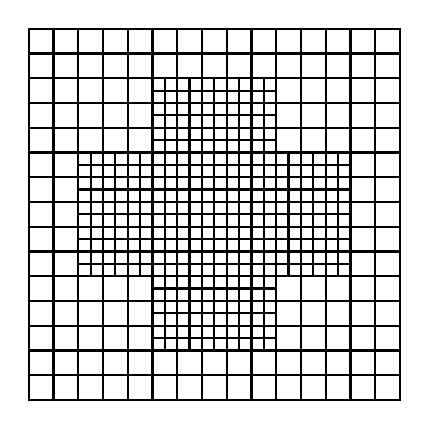
\begin{tikzpicture}[scale=1.5]
\coordinate (v1_1) at (0.0, 0.0);
\coordinate (v1_2) at (0.20943951023931953, 0.0);
\coordinate (v1_3) at (0.20943951023931953, 0.20943951023931953);
\coordinate (v1_4) at (0.0, 0.20943951023931953);
\draw[black, line width=0.8pt] (v1_1) -- (v1_2) -- (v1_3) -- (v1_4) -- cycle;
\coordinate (v2_1) at (0.20943951023931953, 0.0);
\coordinate (v2_2) at (0.41887902047863906, 0.0);
\coordinate (v2_3) at (0.41887902047863906, 0.20943951023931953);
\coordinate (v2_4) at (0.20943951023931953, 0.20943951023931953);
\draw[black, line width=0.8pt] (v2_1) -- (v2_2) -- (v2_3) -- (v2_4) -- cycle;
\coordinate (v3_1) at (0.41887902047863906, 0.0);
\coordinate (v3_2) at (0.6283185307179586, 0.0);
\coordinate (v3_3) at (0.6283185307179586, 0.20943951023931953);
\coordinate (v3_4) at (0.41887902047863906, 0.20943951023931953);
\draw[black, line width=0.8pt] (v3_1) -- (v3_2) -- (v3_3) -- (v3_4) -- cycle;
\coordinate (v4_1) at (0.6283185307179586, 0.0);
\coordinate (v4_2) at (0.8377580409572781, 0.0);
\coordinate (v4_3) at (0.8377580409572781, 0.20943951023931953);
\coordinate (v4_4) at (0.6283185307179586, 0.20943951023931953);
\draw[black, line width=0.8pt] (v4_1) -- (v4_2) -- (v4_3) -- (v4_4) -- cycle;
\coordinate (v5_1) at (0.8377580409572781, 0.0);
\coordinate (v5_2) at (1.0471975511965976, 0.0);
\coordinate (v5_3) at (1.0471975511965976, 0.20943951023931953);
\coordinate (v5_4) at (0.8377580409572781, 0.20943951023931953);
\draw[black, line width=0.8pt] (v5_1) -- (v5_2) -- (v5_3) -- (v5_4) -- cycle;
\coordinate (v6_1) at (1.0471975511965976, 0.0);
\coordinate (v6_2) at (1.2566370614359172, 0.0);
\coordinate (v6_3) at (1.2566370614359172, 0.20943951023931953);
\coordinate (v6_4) at (1.0471975511965976, 0.20943951023931953);
\draw[black, line width=0.8pt] (v6_1) -- (v6_2) -- (v6_3) -- (v6_4) -- cycle;
\coordinate (v7_1) at (1.2566370614359172, 0.0);
\coordinate (v7_2) at (1.4660765716752369, 0.0);
\coordinate (v7_3) at (1.4660765716752369, 0.20943951023931953);
\coordinate (v7_4) at (1.2566370614359172, 0.20943951023931953);
\draw[black, line width=0.8pt] (v7_1) -- (v7_2) -- (v7_3) -- (v7_4) -- cycle;
\coordinate (v8_1) at (1.4660765716752369, 0.0);
\coordinate (v8_2) at (1.6755160819145563, 0.0);
\coordinate (v8_3) at (1.6755160819145563, 0.20943951023931953);
\coordinate (v8_4) at (1.4660765716752369, 0.20943951023931953);
\draw[black, line width=0.8pt] (v8_1) -- (v8_2) -- (v8_3) -- (v8_4) -- cycle;
\coordinate (v9_1) at (1.6755160819145563, 0.0);
\coordinate (v9_2) at (1.8849555921538759, 0.0);
\coordinate (v9_3) at (1.8849555921538759, 0.20943951023931953);
\coordinate (v9_4) at (1.6755160819145563, 0.20943951023931953);
\draw[black, line width=0.8pt] (v9_1) -- (v9_2) -- (v9_3) -- (v9_4) -- cycle;
\coordinate (v10_1) at (1.8849555921538759, 0.0);
\coordinate (v10_2) at (2.0943951023931953, 0.0);
\coordinate (v10_3) at (2.0943951023931953, 0.20943951023931953);
\coordinate (v10_4) at (1.8849555921538759, 0.20943951023931953);
\draw[black, line width=0.8pt] (v10_1) -- (v10_2) -- (v10_3) -- (v10_4) -- cycle;
\coordinate (v11_1) at (2.0943951023931953, 0.0);
\coordinate (v11_2) at (2.3038346126325147, 0.0);
\coordinate (v11_3) at (2.3038346126325147, 0.20943951023931953);
\coordinate (v11_4) at (2.0943951023931953, 0.20943951023931953);
\draw[black, line width=0.8pt] (v11_1) -- (v11_2) -- (v11_3) -- (v11_4) -- cycle;
\coordinate (v12_1) at (2.3038346126325147, 0.0);
\coordinate (v12_2) at (2.5132741228718345, 0.0);
\coordinate (v12_3) at (2.5132741228718345, 0.20943951023931953);
\coordinate (v12_4) at (2.3038346126325147, 0.20943951023931953);
\draw[black, line width=0.8pt] (v12_1) -- (v12_2) -- (v12_3) -- (v12_4) -- cycle;
\coordinate (v13_1) at (2.5132741228718345, 0.0);
\coordinate (v13_2) at (2.7227136331111543, 0.0);
\coordinate (v13_3) at (2.7227136331111543, 0.20943951023931953);
\coordinate (v13_4) at (2.5132741228718345, 0.20943951023931953);
\draw[black, line width=0.8pt] (v13_1) -- (v13_2) -- (v13_3) -- (v13_4) -- cycle;
\coordinate (v14_1) at (2.7227136331111543, 0.0);
\coordinate (v14_2) at (2.9321531433504737, 0.0);
\coordinate (v14_3) at (2.9321531433504737, 0.20943951023931953);
\coordinate (v14_4) at (2.7227136331111543, 0.20943951023931953);
\draw[black, line width=0.8pt] (v14_1) -- (v14_2) -- (v14_3) -- (v14_4) -- cycle;
\coordinate (v15_1) at (2.9321531433504737, 0.0);
\coordinate (v15_2) at (3.141592653589793, 0.0);
\coordinate (v15_3) at (3.141592653589793, 0.20943951023931953);
\coordinate (v15_4) at (2.9321531433504737, 0.20943951023931953);
\draw[black, line width=0.8pt] (v15_1) -- (v15_2) -- (v15_3) -- (v15_4) -- cycle;
\coordinate (v16_1) at (0.0, 0.20943951023931953);
\coordinate (v16_2) at (0.20943951023931953, 0.20943951023931953);
\coordinate (v16_3) at (0.20943951023931953, 0.41887902047863906);
\coordinate (v16_4) at (0.0, 0.41887902047863906);
\draw[black, line width=0.8pt] (v16_1) -- (v16_2) -- (v16_3) -- (v16_4) -- cycle;
\coordinate (v17_1) at (0.20943951023931953, 0.20943951023931953);
\coordinate (v17_2) at (0.41887902047863906, 0.20943951023931953);
\coordinate (v17_3) at (0.41887902047863906, 0.41887902047863906);
\coordinate (v17_4) at (0.20943951023931953, 0.41887902047863906);
\draw[black, line width=0.8pt] (v17_1) -- (v17_2) -- (v17_3) -- (v17_4) -- cycle;
\coordinate (v18_1) at (0.41887902047863906, 0.20943951023931953);
\coordinate (v18_2) at (0.6283185307179586, 0.20943951023931953);
\coordinate (v18_3) at (0.6283185307179586, 0.41887902047863906);
\coordinate (v18_4) at (0.41887902047863906, 0.41887902047863906);
\draw[black, line width=0.8pt] (v18_1) -- (v18_2) -- (v18_3) -- (v18_4) -- cycle;
\coordinate (v19_1) at (0.6283185307179586, 0.20943951023931953);
\coordinate (v19_2) at (0.8377580409572781, 0.20943951023931953);
\coordinate (v19_3) at (0.8377580409572781, 0.41887902047863906);
\coordinate (v19_4) at (0.6283185307179586, 0.41887902047863906);
\draw[black, line width=0.8pt] (v19_1) -- (v19_2) -- (v19_3) -- (v19_4) -- cycle;
\coordinate (v20_1) at (0.8377580409572781, 0.20943951023931953);
\coordinate (v20_2) at (1.0471975511965976, 0.20943951023931953);
\coordinate (v20_3) at (1.0471975511965976, 0.41887902047863906);
\coordinate (v20_4) at (0.8377580409572781, 0.41887902047863906);
\draw[black, line width=0.8pt] (v20_1) -- (v20_2) -- (v20_3) -- (v20_4) -- cycle;
\coordinate (v21_1) at (1.0471975511965976, 0.20943951023931953);
\coordinate (v21_2) at (1.2566370614359172, 0.20943951023931953);
\coordinate (v21_3) at (1.2566370614359172, 0.41887902047863906);
\coordinate (v21_4) at (1.0471975511965976, 0.41887902047863906);
\draw[black, line width=0.8pt] (v21_1) -- (v21_2) -- (v21_3) -- (v21_4) -- cycle;
\coordinate (v22_1) at (1.2566370614359172, 0.20943951023931953);
\coordinate (v22_2) at (1.4660765716752369, 0.20943951023931953);
\coordinate (v22_3) at (1.4660765716752369, 0.41887902047863906);
\coordinate (v22_4) at (1.2566370614359172, 0.41887902047863906);
\draw[black, line width=0.8pt] (v22_1) -- (v22_2) -- (v22_3) -- (v22_4) -- cycle;
\coordinate (v23_1) at (1.4660765716752369, 0.20943951023931953);
\coordinate (v23_2) at (1.6755160819145563, 0.20943951023931953);
\coordinate (v23_3) at (1.6755160819145563, 0.41887902047863906);
\coordinate (v23_4) at (1.4660765716752369, 0.41887902047863906);
\draw[black, line width=0.8pt] (v23_1) -- (v23_2) -- (v23_3) -- (v23_4) -- cycle;
\coordinate (v24_1) at (1.6755160819145563, 0.20943951023931953);
\coordinate (v24_2) at (1.8849555921538759, 0.20943951023931953);
\coordinate (v24_3) at (1.8849555921538759, 0.41887902047863906);
\coordinate (v24_4) at (1.6755160819145563, 0.41887902047863906);
\draw[black, line width=0.8pt] (v24_1) -- (v24_2) -- (v24_3) -- (v24_4) -- cycle;
\coordinate (v25_1) at (1.8849555921538759, 0.20943951023931953);
\coordinate (v25_2) at (2.0943951023931953, 0.20943951023931953);
\coordinate (v25_3) at (2.0943951023931953, 0.41887902047863906);
\coordinate (v25_4) at (1.8849555921538759, 0.41887902047863906);
\draw[black, line width=0.8pt] (v25_1) -- (v25_2) -- (v25_3) -- (v25_4) -- cycle;
\coordinate (v26_1) at (2.0943951023931953, 0.20943951023931953);
\coordinate (v26_2) at (2.3038346126325147, 0.20943951023931953);
\coordinate (v26_3) at (2.3038346126325147, 0.41887902047863906);
\coordinate (v26_4) at (2.0943951023931953, 0.41887902047863906);
\draw[black, line width=0.8pt] (v26_1) -- (v26_2) -- (v26_3) -- (v26_4) -- cycle;
\coordinate (v27_1) at (2.3038346126325147, 0.20943951023931953);
\coordinate (v27_2) at (2.5132741228718345, 0.20943951023931953);
\coordinate (v27_3) at (2.5132741228718345, 0.41887902047863906);
\coordinate (v27_4) at (2.3038346126325147, 0.41887902047863906);
\draw[black, line width=0.8pt] (v27_1) -- (v27_2) -- (v27_3) -- (v27_4) -- cycle;
\coordinate (v28_1) at (2.5132741228718345, 0.20943951023931953);
\coordinate (v28_2) at (2.7227136331111543, 0.20943951023931953);
\coordinate (v28_3) at (2.7227136331111543, 0.41887902047863906);
\coordinate (v28_4) at (2.5132741228718345, 0.41887902047863906);
\draw[black, line width=0.8pt] (v28_1) -- (v28_2) -- (v28_3) -- (v28_4) -- cycle;
\coordinate (v29_1) at (2.7227136331111543, 0.20943951023931953);
\coordinate (v29_2) at (2.9321531433504737, 0.20943951023931953);
\coordinate (v29_3) at (2.9321531433504737, 0.41887902047863906);
\coordinate (v29_4) at (2.7227136331111543, 0.41887902047863906);
\draw[black, line width=0.8pt] (v29_1) -- (v29_2) -- (v29_3) -- (v29_4) -- cycle;
\coordinate (v30_1) at (2.9321531433504737, 0.20943951023931953);
\coordinate (v30_2) at (3.141592653589793, 0.20943951023931953);
\coordinate (v30_3) at (3.141592653589793, 0.41887902047863906);
\coordinate (v30_4) at (2.9321531433504737, 0.41887902047863906);
\draw[black, line width=0.8pt] (v30_1) -- (v30_2) -- (v30_3) -- (v30_4) -- cycle;
\coordinate (v31_1) at (0.0, 0.41887902047863906);
\coordinate (v31_2) at (0.20943951023931953, 0.41887902047863906);
\coordinate (v31_3) at (0.20943951023931953, 0.6283185307179586);
\coordinate (v31_4) at (0.0, 0.6283185307179586);
\draw[black, line width=0.8pt] (v31_1) -- (v31_2) -- (v31_3) -- (v31_4) -- cycle;
\coordinate (v32_1) at (0.20943951023931953, 0.41887902047863906);
\coordinate (v32_2) at (0.41887902047863906, 0.41887902047863906);
\coordinate (v32_3) at (0.41887902047863906, 0.6283185307179586);
\coordinate (v32_4) at (0.20943951023931953, 0.6283185307179586);
\draw[black, line width=0.8pt] (v32_1) -- (v32_2) -- (v32_3) -- (v32_4) -- cycle;
\coordinate (v33_1) at (0.41887902047863906, 0.41887902047863906);
\coordinate (v33_2) at (0.6283185307179586, 0.41887902047863906);
\coordinate (v33_3) at (0.6283185307179586, 0.6283185307179586);
\coordinate (v33_4) at (0.41887902047863906, 0.6283185307179586);
\draw[black, line width=0.8pt] (v33_1) -- (v33_2) -- (v33_3) -- (v33_4) -- cycle;
\coordinate (v34_1) at (0.6283185307179586, 0.41887902047863906);
\coordinate (v34_2) at (0.8377580409572781, 0.41887902047863906);
\coordinate (v34_3) at (0.8377580409572781, 0.6283185307179586);
\coordinate (v34_4) at (0.6283185307179586, 0.6283185307179586);
\draw[black, line width=0.8pt] (v34_1) -- (v34_2) -- (v34_3) -- (v34_4) -- cycle;
\coordinate (v35_1) at (0.8377580409572781, 0.41887902047863906);
\coordinate (v35_2) at (1.0471975511965976, 0.41887902047863906);
\coordinate (v35_3) at (1.0471975511965976, 0.6283185307179586);
\coordinate (v35_4) at (0.8377580409572781, 0.6283185307179586);
\draw[black, line width=0.8pt] (v35_1) -- (v35_2) -- (v35_3) -- (v35_4) -- cycle;
\coordinate (v36_1) at (2.0943951023931953, 0.41887902047863906);
\coordinate (v36_2) at (2.3038346126325147, 0.41887902047863906);
\coordinate (v36_3) at (2.3038346126325147, 0.6283185307179586);
\coordinate (v36_4) at (2.0943951023931953, 0.6283185307179586);
\draw[black, line width=0.8pt] (v36_1) -- (v36_2) -- (v36_3) -- (v36_4) -- cycle;
\coordinate (v37_1) at (2.3038346126325147, 0.41887902047863906);
\coordinate (v37_2) at (2.5132741228718345, 0.41887902047863906);
\coordinate (v37_3) at (2.5132741228718345, 0.6283185307179586);
\coordinate (v37_4) at (2.3038346126325147, 0.6283185307179586);
\draw[black, line width=0.8pt] (v37_1) -- (v37_2) -- (v37_3) -- (v37_4) -- cycle;
\coordinate (v38_1) at (2.5132741228718345, 0.41887902047863906);
\coordinate (v38_2) at (2.7227136331111543, 0.41887902047863906);
\coordinate (v38_3) at (2.7227136331111543, 0.6283185307179586);
\coordinate (v38_4) at (2.5132741228718345, 0.6283185307179586);
\draw[black, line width=0.8pt] (v38_1) -- (v38_2) -- (v38_3) -- (v38_4) -- cycle;
\coordinate (v39_1) at (2.7227136331111543, 0.41887902047863906);
\coordinate (v39_2) at (2.9321531433504737, 0.41887902047863906);
\coordinate (v39_3) at (2.9321531433504737, 0.6283185307179586);
\coordinate (v39_4) at (2.7227136331111543, 0.6283185307179586);
\draw[black, line width=0.8pt] (v39_1) -- (v39_2) -- (v39_3) -- (v39_4) -- cycle;
\coordinate (v40_1) at (2.9321531433504737, 0.41887902047863906);
\coordinate (v40_2) at (3.141592653589793, 0.41887902047863906);
\coordinate (v40_3) at (3.141592653589793, 0.6283185307179586);
\coordinate (v40_4) at (2.9321531433504737, 0.6283185307179586);
\draw[black, line width=0.8pt] (v40_1) -- (v40_2) -- (v40_3) -- (v40_4) -- cycle;
\coordinate (v41_1) at (0.0, 0.6283185307179586);
\coordinate (v41_2) at (0.20943951023931953, 0.6283185307179586);
\coordinate (v41_3) at (0.20943951023931953, 0.8377580409572781);
\coordinate (v41_4) at (0.0, 0.8377580409572781);
\draw[black, line width=0.8pt] (v41_1) -- (v41_2) -- (v41_3) -- (v41_4) -- cycle;
\coordinate (v42_1) at (0.20943951023931953, 0.6283185307179586);
\coordinate (v42_2) at (0.41887902047863906, 0.6283185307179586);
\coordinate (v42_3) at (0.41887902047863906, 0.8377580409572781);
\coordinate (v42_4) at (0.20943951023931953, 0.8377580409572781);
\draw[black, line width=0.8pt] (v42_1) -- (v42_2) -- (v42_3) -- (v42_4) -- cycle;
\coordinate (v43_1) at (0.41887902047863906, 0.6283185307179586);
\coordinate (v43_2) at (0.6283185307179586, 0.6283185307179586);
\coordinate (v43_3) at (0.6283185307179586, 0.8377580409572781);
\coordinate (v43_4) at (0.41887902047863906, 0.8377580409572781);
\draw[black, line width=0.8pt] (v43_1) -- (v43_2) -- (v43_3) -- (v43_4) -- cycle;
\coordinate (v44_1) at (0.6283185307179586, 0.6283185307179586);
\coordinate (v44_2) at (0.8377580409572781, 0.6283185307179586);
\coordinate (v44_3) at (0.8377580409572781, 0.8377580409572781);
\coordinate (v44_4) at (0.6283185307179586, 0.8377580409572781);
\draw[black, line width=0.8pt] (v44_1) -- (v44_2) -- (v44_3) -- (v44_4) -- cycle;
\coordinate (v45_1) at (0.8377580409572781, 0.6283185307179586);
\coordinate (v45_2) at (1.0471975511965976, 0.6283185307179586);
\coordinate (v45_3) at (1.0471975511965976, 0.8377580409572781);
\coordinate (v45_4) at (0.8377580409572781, 0.8377580409572781);
\draw[black, line width=0.8pt] (v45_1) -- (v45_2) -- (v45_3) -- (v45_4) -- cycle;
\coordinate (v46_1) at (2.0943951023931953, 0.6283185307179586);
\coordinate (v46_2) at (2.3038346126325147, 0.6283185307179586);
\coordinate (v46_3) at (2.3038346126325147, 0.8377580409572781);
\coordinate (v46_4) at (2.0943951023931953, 0.8377580409572781);
\draw[black, line width=0.8pt] (v46_1) -- (v46_2) -- (v46_3) -- (v46_4) -- cycle;
\coordinate (v47_1) at (2.3038346126325147, 0.6283185307179586);
\coordinate (v47_2) at (2.5132741228718345, 0.6283185307179586);
\coordinate (v47_3) at (2.5132741228718345, 0.8377580409572781);
\coordinate (v47_4) at (2.3038346126325147, 0.8377580409572781);
\draw[black, line width=0.8pt] (v47_1) -- (v47_2) -- (v47_3) -- (v47_4) -- cycle;
\coordinate (v48_1) at (2.5132741228718345, 0.6283185307179586);
\coordinate (v48_2) at (2.7227136331111543, 0.6283185307179586);
\coordinate (v48_3) at (2.7227136331111543, 0.8377580409572781);
\coordinate (v48_4) at (2.5132741228718345, 0.8377580409572781);
\draw[black, line width=0.8pt] (v48_1) -- (v48_2) -- (v48_3) -- (v48_4) -- cycle;
\coordinate (v49_1) at (2.7227136331111543, 0.6283185307179586);
\coordinate (v49_2) at (2.9321531433504737, 0.6283185307179586);
\coordinate (v49_3) at (2.9321531433504737, 0.8377580409572781);
\coordinate (v49_4) at (2.7227136331111543, 0.8377580409572781);
\draw[black, line width=0.8pt] (v49_1) -- (v49_2) -- (v49_3) -- (v49_4) -- cycle;
\coordinate (v50_1) at (2.9321531433504737, 0.6283185307179586);
\coordinate (v50_2) at (3.141592653589793, 0.6283185307179586);
\coordinate (v50_3) at (3.141592653589793, 0.8377580409572781);
\coordinate (v50_4) at (2.9321531433504737, 0.8377580409572781);
\draw[black, line width=0.8pt] (v50_1) -- (v50_2) -- (v50_3) -- (v50_4) -- cycle;
\coordinate (v51_1) at (0.0, 0.8377580409572781);
\coordinate (v51_2) at (0.20943951023931953, 0.8377580409572781);
\coordinate (v51_3) at (0.20943951023931953, 1.0471975511965976);
\coordinate (v51_4) at (0.0, 1.0471975511965976);
\draw[black, line width=0.8pt] (v51_1) -- (v51_2) -- (v51_3) -- (v51_4) -- cycle;
\coordinate (v52_1) at (0.20943951023931953, 0.8377580409572781);
\coordinate (v52_2) at (0.41887902047863906, 0.8377580409572781);
\coordinate (v52_3) at (0.41887902047863906, 1.0471975511965976);
\coordinate (v52_4) at (0.20943951023931953, 1.0471975511965976);
\draw[black, line width=0.8pt] (v52_1) -- (v52_2) -- (v52_3) -- (v52_4) -- cycle;
\coordinate (v53_1) at (0.41887902047863906, 0.8377580409572781);
\coordinate (v53_2) at (0.6283185307179586, 0.8377580409572781);
\coordinate (v53_3) at (0.6283185307179586, 1.0471975511965976);
\coordinate (v53_4) at (0.41887902047863906, 1.0471975511965976);
\draw[black, line width=0.8pt] (v53_1) -- (v53_2) -- (v53_3) -- (v53_4) -- cycle;
\coordinate (v54_1) at (0.6283185307179586, 0.8377580409572781);
\coordinate (v54_2) at (0.8377580409572781, 0.8377580409572781);
\coordinate (v54_3) at (0.8377580409572781, 1.0471975511965976);
\coordinate (v54_4) at (0.6283185307179586, 1.0471975511965976);
\draw[black, line width=0.8pt] (v54_1) -- (v54_2) -- (v54_3) -- (v54_4) -- cycle;
\coordinate (v55_1) at (0.8377580409572781, 0.8377580409572781);
\coordinate (v55_2) at (1.0471975511965976, 0.8377580409572781);
\coordinate (v55_3) at (1.0471975511965976, 1.0471975511965976);
\coordinate (v55_4) at (0.8377580409572781, 1.0471975511965976);
\draw[black, line width=0.8pt] (v55_1) -- (v55_2) -- (v55_3) -- (v55_4) -- cycle;
\coordinate (v56_1) at (2.0943951023931953, 0.8377580409572781);
\coordinate (v56_2) at (2.3038346126325147, 0.8377580409572781);
\coordinate (v56_3) at (2.3038346126325147, 1.0471975511965976);
\coordinate (v56_4) at (2.0943951023931953, 1.0471975511965976);
\draw[black, line width=0.8pt] (v56_1) -- (v56_2) -- (v56_3) -- (v56_4) -- cycle;
\coordinate (v57_1) at (2.3038346126325147, 0.8377580409572781);
\coordinate (v57_2) at (2.5132741228718345, 0.8377580409572781);
\coordinate (v57_3) at (2.5132741228718345, 1.0471975511965976);
\coordinate (v57_4) at (2.3038346126325147, 1.0471975511965976);
\draw[black, line width=0.8pt] (v57_1) -- (v57_2) -- (v57_3) -- (v57_4) -- cycle;
\coordinate (v58_1) at (2.5132741228718345, 0.8377580409572781);
\coordinate (v58_2) at (2.7227136331111543, 0.8377580409572781);
\coordinate (v58_3) at (2.7227136331111543, 1.0471975511965976);
\coordinate (v58_4) at (2.5132741228718345, 1.0471975511965976);
\draw[black, line width=0.8pt] (v58_1) -- (v58_2) -- (v58_3) -- (v58_4) -- cycle;
\coordinate (v59_1) at (2.7227136331111543, 0.8377580409572781);
\coordinate (v59_2) at (2.9321531433504737, 0.8377580409572781);
\coordinate (v59_3) at (2.9321531433504737, 1.0471975511965976);
\coordinate (v59_4) at (2.7227136331111543, 1.0471975511965976);
\draw[black, line width=0.8pt] (v59_1) -- (v59_2) -- (v59_3) -- (v59_4) -- cycle;
\coordinate (v60_1) at (2.9321531433504737, 0.8377580409572781);
\coordinate (v60_2) at (3.141592653589793, 0.8377580409572781);
\coordinate (v60_3) at (3.141592653589793, 1.0471975511965976);
\coordinate (v60_4) at (2.9321531433504737, 1.0471975511965976);
\draw[black, line width=0.8pt] (v60_1) -- (v60_2) -- (v60_3) -- (v60_4) -- cycle;
\coordinate (v61_1) at (0.0, 1.0471975511965976);
\coordinate (v61_2) at (0.20943951023931953, 1.0471975511965976);
\coordinate (v61_3) at (0.20943951023931953, 1.2566370614359172);
\coordinate (v61_4) at (0.0, 1.2566370614359172);
\draw[black, line width=0.8pt] (v61_1) -- (v61_2) -- (v61_3) -- (v61_4) -- cycle;
\coordinate (v62_1) at (0.20943951023931953, 1.0471975511965976);
\coordinate (v62_2) at (0.41887902047863906, 1.0471975511965976);
\coordinate (v62_3) at (0.41887902047863906, 1.2566370614359172);
\coordinate (v62_4) at (0.20943951023931953, 1.2566370614359172);
\draw[black, line width=0.8pt] (v62_1) -- (v62_2) -- (v62_3) -- (v62_4) -- cycle;
\coordinate (v63_1) at (2.7227136331111543, 1.0471975511965976);
\coordinate (v63_2) at (2.9321531433504737, 1.0471975511965976);
\coordinate (v63_3) at (2.9321531433504737, 1.2566370614359172);
\coordinate (v63_4) at (2.7227136331111543, 1.2566370614359172);
\draw[black, line width=0.8pt] (v63_1) -- (v63_2) -- (v63_3) -- (v63_4) -- cycle;
\coordinate (v64_1) at (2.9321531433504737, 1.0471975511965976);
\coordinate (v64_2) at (3.141592653589793, 1.0471975511965976);
\coordinate (v64_3) at (3.141592653589793, 1.2566370614359172);
\coordinate (v64_4) at (2.9321531433504737, 1.2566370614359172);
\draw[black, line width=0.8pt] (v64_1) -- (v64_2) -- (v64_3) -- (v64_4) -- cycle;
\coordinate (v65_1) at (0.0, 1.2566370614359172);
\coordinate (v65_2) at (0.20943951023931953, 1.2566370614359172);
\coordinate (v65_3) at (0.20943951023931953, 1.4660765716752369);
\coordinate (v65_4) at (0.0, 1.4660765716752369);
\draw[black, line width=0.8pt] (v65_1) -- (v65_2) -- (v65_3) -- (v65_4) -- cycle;
\coordinate (v66_1) at (0.20943951023931953, 1.2566370614359172);
\coordinate (v66_2) at (0.41887902047863906, 1.2566370614359172);
\coordinate (v66_3) at (0.41887902047863906, 1.4660765716752369);
\coordinate (v66_4) at (0.20943951023931953, 1.4660765716752369);
\draw[black, line width=0.8pt] (v66_1) -- (v66_2) -- (v66_3) -- (v66_4) -- cycle;
\coordinate (v67_1) at (2.7227136331111543, 1.2566370614359172);
\coordinate (v67_2) at (2.9321531433504737, 1.2566370614359172);
\coordinate (v67_3) at (2.9321531433504737, 1.4660765716752369);
\coordinate (v67_4) at (2.7227136331111543, 1.4660765716752369);
\draw[black, line width=0.8pt] (v67_1) -- (v67_2) -- (v67_3) -- (v67_4) -- cycle;
\coordinate (v68_1) at (2.9321531433504737, 1.2566370614359172);
\coordinate (v68_2) at (3.141592653589793, 1.2566370614359172);
\coordinate (v68_3) at (3.141592653589793, 1.4660765716752369);
\coordinate (v68_4) at (2.9321531433504737, 1.4660765716752369);
\draw[black, line width=0.8pt] (v68_1) -- (v68_2) -- (v68_3) -- (v68_4) -- cycle;
\coordinate (v69_1) at (0.0, 1.4660765716752369);
\coordinate (v69_2) at (0.20943951023931953, 1.4660765716752369);
\coordinate (v69_3) at (0.20943951023931953, 1.6755160819145563);
\coordinate (v69_4) at (0.0, 1.6755160819145563);
\draw[black, line width=0.8pt] (v69_1) -- (v69_2) -- (v69_3) -- (v69_4) -- cycle;
\coordinate (v70_1) at (0.20943951023931953, 1.4660765716752369);
\coordinate (v70_2) at (0.41887902047863906, 1.4660765716752369);
\coordinate (v70_3) at (0.41887902047863906, 1.6755160819145563);
\coordinate (v70_4) at (0.20943951023931953, 1.6755160819145563);
\draw[black, line width=0.8pt] (v70_1) -- (v70_2) -- (v70_3) -- (v70_4) -- cycle;
\coordinate (v71_1) at (2.7227136331111543, 1.4660765716752369);
\coordinate (v71_2) at (2.9321531433504737, 1.4660765716752369);
\coordinate (v71_3) at (2.9321531433504737, 1.6755160819145563);
\coordinate (v71_4) at (2.7227136331111543, 1.6755160819145563);
\draw[black, line width=0.8pt] (v71_1) -- (v71_2) -- (v71_3) -- (v71_4) -- cycle;
\coordinate (v72_1) at (2.9321531433504737, 1.4660765716752369);
\coordinate (v72_2) at (3.141592653589793, 1.4660765716752369);
\coordinate (v72_3) at (3.141592653589793, 1.6755160819145563);
\coordinate (v72_4) at (2.9321531433504737, 1.6755160819145563);
\draw[black, line width=0.8pt] (v72_1) -- (v72_2) -- (v72_3) -- (v72_4) -- cycle;
\coordinate (v73_1) at (0.0, 1.6755160819145563);
\coordinate (v73_2) at (0.20943951023931953, 1.6755160819145563);
\coordinate (v73_3) at (0.20943951023931953, 1.8849555921538759);
\coordinate (v73_4) at (0.0, 1.8849555921538759);
\draw[black, line width=0.8pt] (v73_1) -- (v73_2) -- (v73_3) -- (v73_4) -- cycle;
\coordinate (v74_1) at (0.20943951023931953, 1.6755160819145563);
\coordinate (v74_2) at (0.41887902047863906, 1.6755160819145563);
\coordinate (v74_3) at (0.41887902047863906, 1.8849555921538759);
\coordinate (v74_4) at (0.20943951023931953, 1.8849555921538759);
\draw[black, line width=0.8pt] (v74_1) -- (v74_2) -- (v74_3) -- (v74_4) -- cycle;
\coordinate (v75_1) at (2.7227136331111543, 1.6755160819145563);
\coordinate (v75_2) at (2.9321531433504737, 1.6755160819145563);
\coordinate (v75_3) at (2.9321531433504737, 1.8849555921538759);
\coordinate (v75_4) at (2.7227136331111543, 1.8849555921538759);
\draw[black, line width=0.8pt] (v75_1) -- (v75_2) -- (v75_3) -- (v75_4) -- cycle;
\coordinate (v76_1) at (2.9321531433504737, 1.6755160819145563);
\coordinate (v76_2) at (3.141592653589793, 1.6755160819145563);
\coordinate (v76_3) at (3.141592653589793, 1.8849555921538759);
\coordinate (v76_4) at (2.9321531433504737, 1.8849555921538759);
\draw[black, line width=0.8pt] (v76_1) -- (v76_2) -- (v76_3) -- (v76_4) -- cycle;
\coordinate (v77_1) at (0.0, 1.8849555921538759);
\coordinate (v77_2) at (0.20943951023931953, 1.8849555921538759);
\coordinate (v77_3) at (0.20943951023931953, 2.0943951023931953);
\coordinate (v77_4) at (0.0, 2.0943951023931953);
\draw[black, line width=0.8pt] (v77_1) -- (v77_2) -- (v77_3) -- (v77_4) -- cycle;
\coordinate (v78_1) at (0.20943951023931953, 1.8849555921538759);
\coordinate (v78_2) at (0.41887902047863906, 1.8849555921538759);
\coordinate (v78_3) at (0.41887902047863906, 2.0943951023931953);
\coordinate (v78_4) at (0.20943951023931953, 2.0943951023931953);
\draw[black, line width=0.8pt] (v78_1) -- (v78_2) -- (v78_3) -- (v78_4) -- cycle;
\coordinate (v79_1) at (2.7227136331111543, 1.8849555921538759);
\coordinate (v79_2) at (2.9321531433504737, 1.8849555921538759);
\coordinate (v79_3) at (2.9321531433504737, 2.0943951023931953);
\coordinate (v79_4) at (2.7227136331111543, 2.0943951023931953);
\draw[black, line width=0.8pt] (v79_1) -- (v79_2) -- (v79_3) -- (v79_4) -- cycle;
\coordinate (v80_1) at (2.9321531433504737, 1.8849555921538759);
\coordinate (v80_2) at (3.141592653589793, 1.8849555921538759);
\coordinate (v80_3) at (3.141592653589793, 2.0943951023931953);
\coordinate (v80_4) at (2.9321531433504737, 2.0943951023931953);
\draw[black, line width=0.8pt] (v80_1) -- (v80_2) -- (v80_3) -- (v80_4) -- cycle;
\coordinate (v81_1) at (0.0, 2.0943951023931953);
\coordinate (v81_2) at (0.20943951023931953, 2.0943951023931953);
\coordinate (v81_3) at (0.20943951023931953, 2.3038346126325147);
\coordinate (v81_4) at (0.0, 2.3038346126325147);
\draw[black, line width=0.8pt] (v81_1) -- (v81_2) -- (v81_3) -- (v81_4) -- cycle;
\coordinate (v82_1) at (0.20943951023931953, 2.0943951023931953);
\coordinate (v82_2) at (0.41887902047863906, 2.0943951023931953);
\coordinate (v82_3) at (0.41887902047863906, 2.3038346126325147);
\coordinate (v82_4) at (0.20943951023931953, 2.3038346126325147);
\draw[black, line width=0.8pt] (v82_1) -- (v82_2) -- (v82_3) -- (v82_4) -- cycle;
\coordinate (v83_1) at (0.41887902047863906, 2.0943951023931953);
\coordinate (v83_2) at (0.6283185307179586, 2.0943951023931953);
\coordinate (v83_3) at (0.6283185307179586, 2.3038346126325147);
\coordinate (v83_4) at (0.41887902047863906, 2.3038346126325147);
\draw[black, line width=0.8pt] (v83_1) -- (v83_2) -- (v83_3) -- (v83_4) -- cycle;
\coordinate (v84_1) at (0.6283185307179586, 2.0943951023931953);
\coordinate (v84_2) at (0.8377580409572781, 2.0943951023931953);
\coordinate (v84_3) at (0.8377580409572781, 2.3038346126325147);
\coordinate (v84_4) at (0.6283185307179586, 2.3038346126325147);
\draw[black, line width=0.8pt] (v84_1) -- (v84_2) -- (v84_3) -- (v84_4) -- cycle;
\coordinate (v85_1) at (0.8377580409572781, 2.0943951023931953);
\coordinate (v85_2) at (1.0471975511965976, 2.0943951023931953);
\coordinate (v85_3) at (1.0471975511965976, 2.3038346126325147);
\coordinate (v85_4) at (0.8377580409572781, 2.3038346126325147);
\draw[black, line width=0.8pt] (v85_1) -- (v85_2) -- (v85_3) -- (v85_4) -- cycle;
\coordinate (v86_1) at (2.0943951023931953, 2.0943951023931953);
\coordinate (v86_2) at (2.3038346126325147, 2.0943951023931953);
\coordinate (v86_3) at (2.3038346126325147, 2.3038346126325147);
\coordinate (v86_4) at (2.0943951023931953, 2.3038346126325147);
\draw[black, line width=0.8pt] (v86_1) -- (v86_2) -- (v86_3) -- (v86_4) -- cycle;
\coordinate (v87_1) at (2.3038346126325147, 2.0943951023931953);
\coordinate (v87_2) at (2.5132741228718345, 2.0943951023931953);
\coordinate (v87_3) at (2.5132741228718345, 2.3038346126325147);
\coordinate (v87_4) at (2.3038346126325147, 2.3038346126325147);
\draw[black, line width=0.8pt] (v87_1) -- (v87_2) -- (v87_3) -- (v87_4) -- cycle;
\coordinate (v88_1) at (2.5132741228718345, 2.0943951023931953);
\coordinate (v88_2) at (2.7227136331111543, 2.0943951023931953);
\coordinate (v88_3) at (2.7227136331111543, 2.3038346126325147);
\coordinate (v88_4) at (2.5132741228718345, 2.3038346126325147);
\draw[black, line width=0.8pt] (v88_1) -- (v88_2) -- (v88_3) -- (v88_4) -- cycle;
\coordinate (v89_1) at (2.7227136331111543, 2.0943951023931953);
\coordinate (v89_2) at (2.9321531433504737, 2.0943951023931953);
\coordinate (v89_3) at (2.9321531433504737, 2.3038346126325147);
\coordinate (v89_4) at (2.7227136331111543, 2.3038346126325147);
\draw[black, line width=0.8pt] (v89_1) -- (v89_2) -- (v89_3) -- (v89_4) -- cycle;
\coordinate (v90_1) at (2.9321531433504737, 2.0943951023931953);
\coordinate (v90_2) at (3.141592653589793, 2.0943951023931953);
\coordinate (v90_3) at (3.141592653589793, 2.3038346126325147);
\coordinate (v90_4) at (2.9321531433504737, 2.3038346126325147);
\draw[black, line width=0.8pt] (v90_1) -- (v90_2) -- (v90_3) -- (v90_4) -- cycle;
\coordinate (v91_1) at (0.0, 2.3038346126325147);
\coordinate (v91_2) at (0.20943951023931953, 2.3038346126325147);
\coordinate (v91_3) at (0.20943951023931953, 2.5132741228718345);
\coordinate (v91_4) at (0.0, 2.5132741228718345);
\draw[black, line width=0.8pt] (v91_1) -- (v91_2) -- (v91_3) -- (v91_4) -- cycle;
\coordinate (v92_1) at (0.20943951023931953, 2.3038346126325147);
\coordinate (v92_2) at (0.41887902047863906, 2.3038346126325147);
\coordinate (v92_3) at (0.41887902047863906, 2.5132741228718345);
\coordinate (v92_4) at (0.20943951023931953, 2.5132741228718345);
\draw[black, line width=0.8pt] (v92_1) -- (v92_2) -- (v92_3) -- (v92_4) -- cycle;
\coordinate (v93_1) at (0.41887902047863906, 2.3038346126325147);
\coordinate (v93_2) at (0.6283185307179586, 2.3038346126325147);
\coordinate (v93_3) at (0.6283185307179586, 2.5132741228718345);
\coordinate (v93_4) at (0.41887902047863906, 2.5132741228718345);
\draw[black, line width=0.8pt] (v93_1) -- (v93_2) -- (v93_3) -- (v93_4) -- cycle;
\coordinate (v94_1) at (0.6283185307179586, 2.3038346126325147);
\coordinate (v94_2) at (0.8377580409572781, 2.3038346126325147);
\coordinate (v94_3) at (0.8377580409572781, 2.5132741228718345);
\coordinate (v94_4) at (0.6283185307179586, 2.5132741228718345);
\draw[black, line width=0.8pt] (v94_1) -- (v94_2) -- (v94_3) -- (v94_4) -- cycle;
\coordinate (v95_1) at (0.8377580409572781, 2.3038346126325147);
\coordinate (v95_2) at (1.0471975511965976, 2.3038346126325147);
\coordinate (v95_3) at (1.0471975511965976, 2.5132741228718345);
\coordinate (v95_4) at (0.8377580409572781, 2.5132741228718345);
\draw[black, line width=0.8pt] (v95_1) -- (v95_2) -- (v95_3) -- (v95_4) -- cycle;
\coordinate (v96_1) at (2.0943951023931953, 2.3038346126325147);
\coordinate (v96_2) at (2.3038346126325147, 2.3038346126325147);
\coordinate (v96_3) at (2.3038346126325147, 2.5132741228718345);
\coordinate (v96_4) at (2.0943951023931953, 2.5132741228718345);
\draw[black, line width=0.8pt] (v96_1) -- (v96_2) -- (v96_3) -- (v96_4) -- cycle;
\coordinate (v97_1) at (2.3038346126325147, 2.3038346126325147);
\coordinate (v97_2) at (2.5132741228718345, 2.3038346126325147);
\coordinate (v97_3) at (2.5132741228718345, 2.5132741228718345);
\coordinate (v97_4) at (2.3038346126325147, 2.5132741228718345);
\draw[black, line width=0.8pt] (v97_1) -- (v97_2) -- (v97_3) -- (v97_4) -- cycle;
\coordinate (v98_1) at (2.5132741228718345, 2.3038346126325147);
\coordinate (v98_2) at (2.7227136331111543, 2.3038346126325147);
\coordinate (v98_3) at (2.7227136331111543, 2.5132741228718345);
\coordinate (v98_4) at (2.5132741228718345, 2.5132741228718345);
\draw[black, line width=0.8pt] (v98_1) -- (v98_2) -- (v98_3) -- (v98_4) -- cycle;
\coordinate (v99_1) at (2.7227136331111543, 2.3038346126325147);
\coordinate (v99_2) at (2.9321531433504737, 2.3038346126325147);
\coordinate (v99_3) at (2.9321531433504737, 2.5132741228718345);
\coordinate (v99_4) at (2.7227136331111543, 2.5132741228718345);
\draw[black, line width=0.8pt] (v99_1) -- (v99_2) -- (v99_3) -- (v99_4) -- cycle;
\coordinate (v100_1) at (2.9321531433504737, 2.3038346126325147);
\coordinate (v100_2) at (3.141592653589793, 2.3038346126325147);
\coordinate (v100_3) at (3.141592653589793, 2.5132741228718345);
\coordinate (v100_4) at (2.9321531433504737, 2.5132741228718345);
\draw[black, line width=0.8pt] (v100_1) -- (v100_2) -- (v100_3) -- (v100_4) -- cycle;
\coordinate (v101_1) at (0.0, 2.5132741228718345);
\coordinate (v101_2) at (0.20943951023931953, 2.5132741228718345);
\coordinate (v101_3) at (0.20943951023931953, 2.7227136331111543);
\coordinate (v101_4) at (0.0, 2.7227136331111543);
\draw[black, line width=0.8pt] (v101_1) -- (v101_2) -- (v101_3) -- (v101_4) -- cycle;
\coordinate (v102_1) at (0.20943951023931953, 2.5132741228718345);
\coordinate (v102_2) at (0.41887902047863906, 2.5132741228718345);
\coordinate (v102_3) at (0.41887902047863906, 2.7227136331111543);
\coordinate (v102_4) at (0.20943951023931953, 2.7227136331111543);
\draw[black, line width=0.8pt] (v102_1) -- (v102_2) -- (v102_3) -- (v102_4) -- cycle;
\coordinate (v103_1) at (0.41887902047863906, 2.5132741228718345);
\coordinate (v103_2) at (0.6283185307179586, 2.5132741228718345);
\coordinate (v103_3) at (0.6283185307179586, 2.7227136331111543);
\coordinate (v103_4) at (0.41887902047863906, 2.7227136331111543);
\draw[black, line width=0.8pt] (v103_1) -- (v103_2) -- (v103_3) -- (v103_4) -- cycle;
\coordinate (v104_1) at (0.6283185307179586, 2.5132741228718345);
\coordinate (v104_2) at (0.8377580409572781, 2.5132741228718345);
\coordinate (v104_3) at (0.8377580409572781, 2.7227136331111543);
\coordinate (v104_4) at (0.6283185307179586, 2.7227136331111543);
\draw[black, line width=0.8pt] (v104_1) -- (v104_2) -- (v104_3) -- (v104_4) -- cycle;
\coordinate (v105_1) at (0.8377580409572781, 2.5132741228718345);
\coordinate (v105_2) at (1.0471975511965976, 2.5132741228718345);
\coordinate (v105_3) at (1.0471975511965976, 2.7227136331111543);
\coordinate (v105_4) at (0.8377580409572781, 2.7227136331111543);
\draw[black, line width=0.8pt] (v105_1) -- (v105_2) -- (v105_3) -- (v105_4) -- cycle;
\coordinate (v106_1) at (2.0943951023931953, 2.5132741228718345);
\coordinate (v106_2) at (2.3038346126325147, 2.5132741228718345);
\coordinate (v106_3) at (2.3038346126325147, 2.7227136331111543);
\coordinate (v106_4) at (2.0943951023931953, 2.7227136331111543);
\draw[black, line width=0.8pt] (v106_1) -- (v106_2) -- (v106_3) -- (v106_4) -- cycle;
\coordinate (v107_1) at (2.3038346126325147, 2.5132741228718345);
\coordinate (v107_2) at (2.5132741228718345, 2.5132741228718345);
\coordinate (v107_3) at (2.5132741228718345, 2.7227136331111543);
\coordinate (v107_4) at (2.3038346126325147, 2.7227136331111543);
\draw[black, line width=0.8pt] (v107_1) -- (v107_2) -- (v107_3) -- (v107_4) -- cycle;
\coordinate (v108_1) at (2.5132741228718345, 2.5132741228718345);
\coordinate (v108_2) at (2.7227136331111543, 2.5132741228718345);
\coordinate (v108_3) at (2.7227136331111543, 2.7227136331111543);
\coordinate (v108_4) at (2.5132741228718345, 2.7227136331111543);
\draw[black, line width=0.8pt] (v108_1) -- (v108_2) -- (v108_3) -- (v108_4) -- cycle;
\coordinate (v109_1) at (2.7227136331111543, 2.5132741228718345);
\coordinate (v109_2) at (2.9321531433504737, 2.5132741228718345);
\coordinate (v109_3) at (2.9321531433504737, 2.7227136331111543);
\coordinate (v109_4) at (2.7227136331111543, 2.7227136331111543);
\draw[black, line width=0.8pt] (v109_1) -- (v109_2) -- (v109_3) -- (v109_4) -- cycle;
\coordinate (v110_1) at (2.9321531433504737, 2.5132741228718345);
\coordinate (v110_2) at (3.141592653589793, 2.5132741228718345);
\coordinate (v110_3) at (3.141592653589793, 2.7227136331111543);
\coordinate (v110_4) at (2.9321531433504737, 2.7227136331111543);
\draw[black, line width=0.8pt] (v110_1) -- (v110_2) -- (v110_3) -- (v110_4) -- cycle;
\coordinate (v111_1) at (0.0, 2.7227136331111543);
\coordinate (v111_2) at (0.20943951023931953, 2.7227136331111543);
\coordinate (v111_3) at (0.20943951023931953, 2.9321531433504737);
\coordinate (v111_4) at (0.0, 2.9321531433504737);
\draw[black, line width=0.8pt] (v111_1) -- (v111_2) -- (v111_3) -- (v111_4) -- cycle;
\coordinate (v112_1) at (0.20943951023931953, 2.7227136331111543);
\coordinate (v112_2) at (0.41887902047863906, 2.7227136331111543);
\coordinate (v112_3) at (0.41887902047863906, 2.9321531433504737);
\coordinate (v112_4) at (0.20943951023931953, 2.9321531433504737);
\draw[black, line width=0.8pt] (v112_1) -- (v112_2) -- (v112_3) -- (v112_4) -- cycle;
\coordinate (v113_1) at (0.41887902047863906, 2.7227136331111543);
\coordinate (v113_2) at (0.6283185307179586, 2.7227136331111543);
\coordinate (v113_3) at (0.6283185307179586, 2.9321531433504737);
\coordinate (v113_4) at (0.41887902047863906, 2.9321531433504737);
\draw[black, line width=0.8pt] (v113_1) -- (v113_2) -- (v113_3) -- (v113_4) -- cycle;
\coordinate (v114_1) at (0.6283185307179586, 2.7227136331111543);
\coordinate (v114_2) at (0.8377580409572781, 2.7227136331111543);
\coordinate (v114_3) at (0.8377580409572781, 2.9321531433504737);
\coordinate (v114_4) at (0.6283185307179586, 2.9321531433504737);
\draw[black, line width=0.8pt] (v114_1) -- (v114_2) -- (v114_3) -- (v114_4) -- cycle;
\coordinate (v115_1) at (0.8377580409572781, 2.7227136331111543);
\coordinate (v115_2) at (1.0471975511965976, 2.7227136331111543);
\coordinate (v115_3) at (1.0471975511965976, 2.9321531433504737);
\coordinate (v115_4) at (0.8377580409572781, 2.9321531433504737);
\draw[black, line width=0.8pt] (v115_1) -- (v115_2) -- (v115_3) -- (v115_4) -- cycle;
\coordinate (v116_1) at (1.0471975511965976, 2.7227136331111543);
\coordinate (v116_2) at (1.2566370614359172, 2.7227136331111543);
\coordinate (v116_3) at (1.2566370614359172, 2.9321531433504737);
\coordinate (v116_4) at (1.0471975511965976, 2.9321531433504737);
\draw[black, line width=0.8pt] (v116_1) -- (v116_2) -- (v116_3) -- (v116_4) -- cycle;
\coordinate (v117_1) at (1.2566370614359172, 2.7227136331111543);
\coordinate (v117_2) at (1.4660765716752369, 2.7227136331111543);
\coordinate (v117_3) at (1.4660765716752369, 2.9321531433504737);
\coordinate (v117_4) at (1.2566370614359172, 2.9321531433504737);
\draw[black, line width=0.8pt] (v117_1) -- (v117_2) -- (v117_3) -- (v117_4) -- cycle;
\coordinate (v118_1) at (1.4660765716752369, 2.7227136331111543);
\coordinate (v118_2) at (1.6755160819145563, 2.7227136331111543);
\coordinate (v118_3) at (1.6755160819145563, 2.9321531433504737);
\coordinate (v118_4) at (1.4660765716752369, 2.9321531433504737);
\draw[black, line width=0.8pt] (v118_1) -- (v118_2) -- (v118_3) -- (v118_4) -- cycle;
\coordinate (v119_1) at (1.6755160819145563, 2.7227136331111543);
\coordinate (v119_2) at (1.8849555921538759, 2.7227136331111543);
\coordinate (v119_3) at (1.8849555921538759, 2.9321531433504737);
\coordinate (v119_4) at (1.6755160819145563, 2.9321531433504737);
\draw[black, line width=0.8pt] (v119_1) -- (v119_2) -- (v119_3) -- (v119_4) -- cycle;
\coordinate (v120_1) at (1.8849555921538759, 2.7227136331111543);
\coordinate (v120_2) at (2.0943951023931953, 2.7227136331111543);
\coordinate (v120_3) at (2.0943951023931953, 2.9321531433504737);
\coordinate (v120_4) at (1.8849555921538759, 2.9321531433504737);
\draw[black, line width=0.8pt] (v120_1) -- (v120_2) -- (v120_3) -- (v120_4) -- cycle;
\coordinate (v121_1) at (2.0943951023931953, 2.7227136331111543);
\coordinate (v121_2) at (2.3038346126325147, 2.7227136331111543);
\coordinate (v121_3) at (2.3038346126325147, 2.9321531433504737);
\coordinate (v121_4) at (2.0943951023931953, 2.9321531433504737);
\draw[black, line width=0.8pt] (v121_1) -- (v121_2) -- (v121_3) -- (v121_4) -- cycle;
\coordinate (v122_1) at (2.3038346126325147, 2.7227136331111543);
\coordinate (v122_2) at (2.5132741228718345, 2.7227136331111543);
\coordinate (v122_3) at (2.5132741228718345, 2.9321531433504737);
\coordinate (v122_4) at (2.3038346126325147, 2.9321531433504737);
\draw[black, line width=0.8pt] (v122_1) -- (v122_2) -- (v122_3) -- (v122_4) -- cycle;
\coordinate (v123_1) at (2.5132741228718345, 2.7227136331111543);
\coordinate (v123_2) at (2.7227136331111543, 2.7227136331111543);
\coordinate (v123_3) at (2.7227136331111543, 2.9321531433504737);
\coordinate (v123_4) at (2.5132741228718345, 2.9321531433504737);
\draw[black, line width=0.8pt] (v123_1) -- (v123_2) -- (v123_3) -- (v123_4) -- cycle;
\coordinate (v124_1) at (2.7227136331111543, 2.7227136331111543);
\coordinate (v124_2) at (2.9321531433504737, 2.7227136331111543);
\coordinate (v124_3) at (2.9321531433504737, 2.9321531433504737);
\coordinate (v124_4) at (2.7227136331111543, 2.9321531433504737);
\draw[black, line width=0.8pt] (v124_1) -- (v124_2) -- (v124_3) -- (v124_4) -- cycle;
\coordinate (v125_1) at (2.9321531433504737, 2.7227136331111543);
\coordinate (v125_2) at (3.141592653589793, 2.7227136331111543);
\coordinate (v125_3) at (3.141592653589793, 2.9321531433504737);
\coordinate (v125_4) at (2.9321531433504737, 2.9321531433504737);
\draw[black, line width=0.8pt] (v125_1) -- (v125_2) -- (v125_3) -- (v125_4) -- cycle;
\coordinate (v126_1) at (0.0, 2.9321531433504737);
\coordinate (v126_2) at (0.20943951023931953, 2.9321531433504737);
\coordinate (v126_3) at (0.20943951023931953, 3.141592653589793);
\coordinate (v126_4) at (0.0, 3.141592653589793);
\draw[black, line width=0.8pt] (v126_1) -- (v126_2) -- (v126_3) -- (v126_4) -- cycle;
\coordinate (v127_1) at (0.20943951023931953, 2.9321531433504737);
\coordinate (v127_2) at (0.41887902047863906, 2.9321531433504737);
\coordinate (v127_3) at (0.41887902047863906, 3.141592653589793);
\coordinate (v127_4) at (0.20943951023931953, 3.141592653589793);
\draw[black, line width=0.8pt] (v127_1) -- (v127_2) -- (v127_3) -- (v127_4) -- cycle;
\coordinate (v128_1) at (0.41887902047863906, 2.9321531433504737);
\coordinate (v128_2) at (0.6283185307179586, 2.9321531433504737);
\coordinate (v128_3) at (0.6283185307179586, 3.141592653589793);
\coordinate (v128_4) at (0.41887902047863906, 3.141592653589793);
\draw[black, line width=0.8pt] (v128_1) -- (v128_2) -- (v128_3) -- (v128_4) -- cycle;
\coordinate (v129_1) at (0.6283185307179586, 2.9321531433504737);
\coordinate (v129_2) at (0.8377580409572781, 2.9321531433504737);
\coordinate (v129_3) at (0.8377580409572781, 3.141592653589793);
\coordinate (v129_4) at (0.6283185307179586, 3.141592653589793);
\draw[black, line width=0.8pt] (v129_1) -- (v129_2) -- (v129_3) -- (v129_4) -- cycle;
\coordinate (v130_1) at (0.8377580409572781, 2.9321531433504737);
\coordinate (v130_2) at (1.0471975511965976, 2.9321531433504737);
\coordinate (v130_3) at (1.0471975511965976, 3.141592653589793);
\coordinate (v130_4) at (0.8377580409572781, 3.141592653589793);
\draw[black, line width=0.8pt] (v130_1) -- (v130_2) -- (v130_3) -- (v130_4) -- cycle;
\coordinate (v131_1) at (1.0471975511965976, 2.9321531433504737);
\coordinate (v131_2) at (1.2566370614359172, 2.9321531433504737);
\coordinate (v131_3) at (1.2566370614359172, 3.141592653589793);
\coordinate (v131_4) at (1.0471975511965976, 3.141592653589793);
\draw[black, line width=0.8pt] (v131_1) -- (v131_2) -- (v131_3) -- (v131_4) -- cycle;
\coordinate (v132_1) at (1.2566370614359172, 2.9321531433504737);
\coordinate (v132_2) at (1.4660765716752369, 2.9321531433504737);
\coordinate (v132_3) at (1.4660765716752369, 3.141592653589793);
\coordinate (v132_4) at (1.2566370614359172, 3.141592653589793);
\draw[black, line width=0.8pt] (v132_1) -- (v132_2) -- (v132_3) -- (v132_4) -- cycle;
\coordinate (v133_1) at (1.4660765716752369, 2.9321531433504737);
\coordinate (v133_2) at (1.6755160819145563, 2.9321531433504737);
\coordinate (v133_3) at (1.6755160819145563, 3.141592653589793);
\coordinate (v133_4) at (1.4660765716752369, 3.141592653589793);
\draw[black, line width=0.8pt] (v133_1) -- (v133_2) -- (v133_3) -- (v133_4) -- cycle;
\coordinate (v134_1) at (1.6755160819145563, 2.9321531433504737);
\coordinate (v134_2) at (1.8849555921538759, 2.9321531433504737);
\coordinate (v134_3) at (1.8849555921538759, 3.141592653589793);
\coordinate (v134_4) at (1.6755160819145563, 3.141592653589793);
\draw[black, line width=0.8pt] (v134_1) -- (v134_2) -- (v134_3) -- (v134_4) -- cycle;
\coordinate (v135_1) at (1.8849555921538759, 2.9321531433504737);
\coordinate (v135_2) at (2.0943951023931953, 2.9321531433504737);
\coordinate (v135_3) at (2.0943951023931953, 3.141592653589793);
\coordinate (v135_4) at (1.8849555921538759, 3.141592653589793);
\draw[black, line width=0.8pt] (v135_1) -- (v135_2) -- (v135_3) -- (v135_4) -- cycle;
\coordinate (v136_1) at (2.0943951023931953, 2.9321531433504737);
\coordinate (v136_2) at (2.3038346126325147, 2.9321531433504737);
\coordinate (v136_3) at (2.3038346126325147, 3.141592653589793);
\coordinate (v136_4) at (2.0943951023931953, 3.141592653589793);
\draw[black, line width=0.8pt] (v136_1) -- (v136_2) -- (v136_3) -- (v136_4) -- cycle;
\coordinate (v137_1) at (2.3038346126325147, 2.9321531433504737);
\coordinate (v137_2) at (2.5132741228718345, 2.9321531433504737);
\coordinate (v137_3) at (2.5132741228718345, 3.141592653589793);
\coordinate (v137_4) at (2.3038346126325147, 3.141592653589793);
\draw[black, line width=0.8pt] (v137_1) -- (v137_2) -- (v137_3) -- (v137_4) -- cycle;
\coordinate (v138_1) at (2.5132741228718345, 2.9321531433504737);
\coordinate (v138_2) at (2.7227136331111543, 2.9321531433504737);
\coordinate (v138_3) at (2.7227136331111543, 3.141592653589793);
\coordinate (v138_4) at (2.5132741228718345, 3.141592653589793);
\draw[black, line width=0.8pt] (v138_1) -- (v138_2) -- (v138_3) -- (v138_4) -- cycle;
\coordinate (v139_1) at (2.7227136331111543, 2.9321531433504737);
\coordinate (v139_2) at (2.9321531433504737, 2.9321531433504737);
\coordinate (v139_3) at (2.9321531433504737, 3.141592653589793);
\coordinate (v139_4) at (2.7227136331111543, 3.141592653589793);
\draw[black, line width=0.8pt] (v139_1) -- (v139_2) -- (v139_3) -- (v139_4) -- cycle;
\coordinate (v140_1) at (2.9321531433504737, 2.9321531433504737);
\coordinate (v140_2) at (3.141592653589793, 2.9321531433504737);
\coordinate (v140_3) at (3.141592653589793, 3.141592653589793);
\coordinate (v140_4) at (2.9321531433504737, 3.141592653589793);
\draw[black, line width=0.8pt] (v140_1) -- (v140_2) -- (v140_3) -- (v140_4) -- cycle;
\coordinate (v141_1) at (1.0471975511965976, 0.41887902047863906);
\coordinate (v141_2) at (1.1519173063162573, 0.41887902047863906);
\coordinate (v141_3) at (1.1519173063162573, 0.5235987755982988);
\coordinate (v141_4) at (1.0471975511965976, 0.5235987755982988);
\draw[black, line width=0.8pt] (v141_1) -- (v141_2) -- (v141_3) -- (v141_4) -- cycle;
\coordinate (v142_1) at (1.1519173063162573, 0.41887902047863906);
\coordinate (v142_2) at (1.2566370614359172, 0.41887902047863906);
\coordinate (v142_3) at (1.2566370614359172, 0.5235987755982988);
\coordinate (v142_4) at (1.1519173063162573, 0.5235987755982988);
\draw[black, line width=0.8pt] (v142_1) -- (v142_2) -- (v142_3) -- (v142_4) -- cycle;
\coordinate (v143_1) at (1.2566370614359172, 0.41887902047863906);
\coordinate (v143_2) at (1.3613568165555772, 0.41887902047863906);
\coordinate (v143_3) at (1.3613568165555772, 0.5235987755982988);
\coordinate (v143_4) at (1.2566370614359172, 0.5235987755982988);
\draw[black, line width=0.8pt] (v143_1) -- (v143_2) -- (v143_3) -- (v143_4) -- cycle;
\coordinate (v144_1) at (1.3613568165555772, 0.41887902047863906);
\coordinate (v144_2) at (1.4660765716752369, 0.41887902047863906);
\coordinate (v144_3) at (1.4660765716752369, 0.5235987755982988);
\coordinate (v144_4) at (1.3613568165555772, 0.5235987755982988);
\draw[black, line width=0.8pt] (v144_1) -- (v144_2) -- (v144_3) -- (v144_4) -- cycle;
\coordinate (v145_1) at (1.4660765716752369, 0.41887902047863906);
\coordinate (v145_2) at (1.5707963267948966, 0.41887902047863906);
\coordinate (v145_3) at (1.5707963267948966, 0.5235987755982988);
\coordinate (v145_4) at (1.4660765716752369, 0.5235987755982988);
\draw[black, line width=0.8pt] (v145_1) -- (v145_2) -- (v145_3) -- (v145_4) -- cycle;
\coordinate (v146_1) at (1.5707963267948966, 0.41887902047863906);
\coordinate (v146_2) at (1.6755160819145563, 0.41887902047863906);
\coordinate (v146_3) at (1.6755160819145563, 0.5235987755982988);
\coordinate (v146_4) at (1.5707963267948966, 0.5235987755982988);
\draw[black, line width=0.8pt] (v146_1) -- (v146_2) -- (v146_3) -- (v146_4) -- cycle;
\coordinate (v147_1) at (1.6755160819145563, 0.41887902047863906);
\coordinate (v147_2) at (1.780235837034216, 0.41887902047863906);
\coordinate (v147_3) at (1.780235837034216, 0.5235987755982988);
\coordinate (v147_4) at (1.6755160819145563, 0.5235987755982988);
\draw[black, line width=0.8pt] (v147_1) -- (v147_2) -- (v147_3) -- (v147_4) -- cycle;
\coordinate (v148_1) at (1.780235837034216, 0.41887902047863906);
\coordinate (v148_2) at (1.8849555921538759, 0.41887902047863906);
\coordinate (v148_3) at (1.8849555921538759, 0.5235987755982988);
\coordinate (v148_4) at (1.780235837034216, 0.5235987755982988);
\draw[black, line width=0.8pt] (v148_1) -- (v148_2) -- (v148_3) -- (v148_4) -- cycle;
\coordinate (v149_1) at (1.8849555921538759, 0.41887902047863906);
\coordinate (v149_2) at (1.9896753472735356, 0.41887902047863906);
\coordinate (v149_3) at (1.9896753472735356, 0.5235987755982988);
\coordinate (v149_4) at (1.8849555921538759, 0.5235987755982988);
\draw[black, line width=0.8pt] (v149_1) -- (v149_2) -- (v149_3) -- (v149_4) -- cycle;
\coordinate (v150_1) at (1.9896753472735356, 0.41887902047863906);
\coordinate (v150_2) at (2.0943951023931953, 0.41887902047863906);
\coordinate (v150_3) at (2.0943951023931953, 0.5235987755982988);
\coordinate (v150_4) at (1.9896753472735356, 0.5235987755982988);
\draw[black, line width=0.8pt] (v150_1) -- (v150_2) -- (v150_3) -- (v150_4) -- cycle;
\coordinate (v151_1) at (1.0471975511965976, 0.5235987755982988);
\coordinate (v151_2) at (1.1519173063162573, 0.5235987755982988);
\coordinate (v151_3) at (1.1519173063162573, 0.6283185307179586);
\coordinate (v151_4) at (1.0471975511965976, 0.6283185307179586);
\draw[black, line width=0.8pt] (v151_1) -- (v151_2) -- (v151_3) -- (v151_4) -- cycle;
\coordinate (v152_1) at (1.1519173063162573, 0.5235987755982988);
\coordinate (v152_2) at (1.2566370614359172, 0.5235987755982988);
\coordinate (v152_3) at (1.2566370614359172, 0.6283185307179586);
\coordinate (v152_4) at (1.1519173063162573, 0.6283185307179586);
\draw[black, line width=0.8pt] (v152_1) -- (v152_2) -- (v152_3) -- (v152_4) -- cycle;
\coordinate (v153_1) at (1.2566370614359172, 0.5235987755982988);
\coordinate (v153_2) at (1.3613568165555772, 0.5235987755982988);
\coordinate (v153_3) at (1.3613568165555772, 0.6283185307179586);
\coordinate (v153_4) at (1.2566370614359172, 0.6283185307179586);
\draw[black, line width=0.8pt] (v153_1) -- (v153_2) -- (v153_3) -- (v153_4) -- cycle;
\coordinate (v154_1) at (1.3613568165555772, 0.5235987755982988);
\coordinate (v154_2) at (1.4660765716752369, 0.5235987755982988);
\coordinate (v154_3) at (1.4660765716752369, 0.6283185307179586);
\coordinate (v154_4) at (1.3613568165555772, 0.6283185307179586);
\draw[black, line width=0.8pt] (v154_1) -- (v154_2) -- (v154_3) -- (v154_4) -- cycle;
\coordinate (v155_1) at (1.4660765716752369, 0.5235987755982988);
\coordinate (v155_2) at (1.5707963267948966, 0.5235987755982988);
\coordinate (v155_3) at (1.5707963267948966, 0.6283185307179586);
\coordinate (v155_4) at (1.4660765716752369, 0.6283185307179586);
\draw[black, line width=0.8pt] (v155_1) -- (v155_2) -- (v155_3) -- (v155_4) -- cycle;
\coordinate (v156_1) at (1.5707963267948966, 0.5235987755982988);
\coordinate (v156_2) at (1.6755160819145563, 0.5235987755982988);
\coordinate (v156_3) at (1.6755160819145563, 0.6283185307179586);
\coordinate (v156_4) at (1.5707963267948966, 0.6283185307179586);
\draw[black, line width=0.8pt] (v156_1) -- (v156_2) -- (v156_3) -- (v156_4) -- cycle;
\coordinate (v157_1) at (1.6755160819145563, 0.5235987755982988);
\coordinate (v157_2) at (1.780235837034216, 0.5235987755982988);
\coordinate (v157_3) at (1.780235837034216, 0.6283185307179586);
\coordinate (v157_4) at (1.6755160819145563, 0.6283185307179586);
\draw[black, line width=0.8pt] (v157_1) -- (v157_2) -- (v157_3) -- (v157_4) -- cycle;
\coordinate (v158_1) at (1.780235837034216, 0.5235987755982988);
\coordinate (v158_2) at (1.8849555921538759, 0.5235987755982988);
\coordinate (v158_3) at (1.8849555921538759, 0.6283185307179586);
\coordinate (v158_4) at (1.780235837034216, 0.6283185307179586);
\draw[black, line width=0.8pt] (v158_1) -- (v158_2) -- (v158_3) -- (v158_4) -- cycle;
\coordinate (v159_1) at (1.8849555921538759, 0.5235987755982988);
\coordinate (v159_2) at (1.9896753472735356, 0.5235987755982988);
\coordinate (v159_3) at (1.9896753472735356, 0.6283185307179586);
\coordinate (v159_4) at (1.8849555921538759, 0.6283185307179586);
\draw[black, line width=0.8pt] (v159_1) -- (v159_2) -- (v159_3) -- (v159_4) -- cycle;
\coordinate (v160_1) at (1.9896753472735356, 0.5235987755982988);
\coordinate (v160_2) at (2.0943951023931953, 0.5235987755982988);
\coordinate (v160_3) at (2.0943951023931953, 0.6283185307179586);
\coordinate (v160_4) at (1.9896753472735356, 0.6283185307179586);
\draw[black, line width=0.8pt] (v160_1) -- (v160_2) -- (v160_3) -- (v160_4) -- cycle;
\coordinate (v161_1) at (1.0471975511965976, 0.6283185307179586);
\coordinate (v161_2) at (1.1519173063162573, 0.6283185307179586);
\coordinate (v161_3) at (1.1519173063162573, 0.7330382858376183);
\coordinate (v161_4) at (1.0471975511965976, 0.7330382858376183);
\draw[black, line width=0.8pt] (v161_1) -- (v161_2) -- (v161_3) -- (v161_4) -- cycle;
\coordinate (v162_1) at (1.1519173063162573, 0.6283185307179586);
\coordinate (v162_2) at (1.2566370614359172, 0.6283185307179586);
\coordinate (v162_3) at (1.2566370614359172, 0.7330382858376183);
\coordinate (v162_4) at (1.1519173063162573, 0.7330382858376183);
\draw[black, line width=0.8pt] (v162_1) -- (v162_2) -- (v162_3) -- (v162_4) -- cycle;
\coordinate (v163_1) at (1.2566370614359172, 0.6283185307179586);
\coordinate (v163_2) at (1.3613568165555772, 0.6283185307179586);
\coordinate (v163_3) at (1.3613568165555772, 0.7330382858376183);
\coordinate (v163_4) at (1.2566370614359172, 0.7330382858376183);
\draw[black, line width=0.8pt] (v163_1) -- (v163_2) -- (v163_3) -- (v163_4) -- cycle;
\coordinate (v164_1) at (1.3613568165555772, 0.6283185307179586);
\coordinate (v164_2) at (1.4660765716752369, 0.6283185307179586);
\coordinate (v164_3) at (1.4660765716752369, 0.7330382858376183);
\coordinate (v164_4) at (1.3613568165555772, 0.7330382858376183);
\draw[black, line width=0.8pt] (v164_1) -- (v164_2) -- (v164_3) -- (v164_4) -- cycle;
\coordinate (v165_1) at (1.4660765716752369, 0.6283185307179586);
\coordinate (v165_2) at (1.5707963267948966, 0.6283185307179586);
\coordinate (v165_3) at (1.5707963267948966, 0.7330382858376183);
\coordinate (v165_4) at (1.4660765716752369, 0.7330382858376183);
\draw[black, line width=0.8pt] (v165_1) -- (v165_2) -- (v165_3) -- (v165_4) -- cycle;
\coordinate (v166_1) at (1.5707963267948966, 0.6283185307179586);
\coordinate (v166_2) at (1.6755160819145563, 0.6283185307179586);
\coordinate (v166_3) at (1.6755160819145563, 0.7330382858376183);
\coordinate (v166_4) at (1.5707963267948966, 0.7330382858376183);
\draw[black, line width=0.8pt] (v166_1) -- (v166_2) -- (v166_3) -- (v166_4) -- cycle;
\coordinate (v167_1) at (1.6755160819145563, 0.6283185307179586);
\coordinate (v167_2) at (1.780235837034216, 0.6283185307179586);
\coordinate (v167_3) at (1.780235837034216, 0.7330382858376183);
\coordinate (v167_4) at (1.6755160819145563, 0.7330382858376183);
\draw[black, line width=0.8pt] (v167_1) -- (v167_2) -- (v167_3) -- (v167_4) -- cycle;
\coordinate (v168_1) at (1.780235837034216, 0.6283185307179586);
\coordinate (v168_2) at (1.8849555921538759, 0.6283185307179586);
\coordinate (v168_3) at (1.8849555921538759, 0.7330382858376183);
\coordinate (v168_4) at (1.780235837034216, 0.7330382858376183);
\draw[black, line width=0.8pt] (v168_1) -- (v168_2) -- (v168_3) -- (v168_4) -- cycle;
\coordinate (v169_1) at (1.8849555921538759, 0.6283185307179586);
\coordinate (v169_2) at (1.9896753472735356, 0.6283185307179586);
\coordinate (v169_3) at (1.9896753472735356, 0.7330382858376183);
\coordinate (v169_4) at (1.8849555921538759, 0.7330382858376183);
\draw[black, line width=0.8pt] (v169_1) -- (v169_2) -- (v169_3) -- (v169_4) -- cycle;
\coordinate (v170_1) at (1.9896753472735356, 0.6283185307179586);
\coordinate (v170_2) at (2.0943951023931953, 0.6283185307179586);
\coordinate (v170_3) at (2.0943951023931953, 0.7330382858376183);
\coordinate (v170_4) at (1.9896753472735356, 0.7330382858376183);
\draw[black, line width=0.8pt] (v170_1) -- (v170_2) -- (v170_3) -- (v170_4) -- cycle;
\coordinate (v171_1) at (1.0471975511965976, 0.7330382858376183);
\coordinate (v171_2) at (1.1519173063162573, 0.7330382858376183);
\coordinate (v171_3) at (1.1519173063162573, 0.8377580409572781);
\coordinate (v171_4) at (1.0471975511965976, 0.8377580409572781);
\draw[black, line width=0.8pt] (v171_1) -- (v171_2) -- (v171_3) -- (v171_4) -- cycle;
\coordinate (v172_1) at (1.1519173063162573, 0.7330382858376183);
\coordinate (v172_2) at (1.2566370614359172, 0.7330382858376183);
\coordinate (v172_3) at (1.2566370614359172, 0.8377580409572781);
\coordinate (v172_4) at (1.1519173063162573, 0.8377580409572781);
\draw[black, line width=0.8pt] (v172_1) -- (v172_2) -- (v172_3) -- (v172_4) -- cycle;
\coordinate (v173_1) at (1.2566370614359172, 0.7330382858376183);
\coordinate (v173_2) at (1.3613568165555772, 0.7330382858376183);
\coordinate (v173_3) at (1.3613568165555772, 0.8377580409572781);
\coordinate (v173_4) at (1.2566370614359172, 0.8377580409572781);
\draw[black, line width=0.8pt] (v173_1) -- (v173_2) -- (v173_3) -- (v173_4) -- cycle;
\coordinate (v174_1) at (1.3613568165555772, 0.7330382858376183);
\coordinate (v174_2) at (1.4660765716752369, 0.7330382858376183);
\coordinate (v174_3) at (1.4660765716752369, 0.8377580409572781);
\coordinate (v174_4) at (1.3613568165555772, 0.8377580409572781);
\draw[black, line width=0.8pt] (v174_1) -- (v174_2) -- (v174_3) -- (v174_4) -- cycle;
\coordinate (v175_1) at (1.4660765716752369, 0.7330382858376183);
\coordinate (v175_2) at (1.5707963267948966, 0.7330382858376183);
\coordinate (v175_3) at (1.5707963267948966, 0.8377580409572781);
\coordinate (v175_4) at (1.4660765716752369, 0.8377580409572781);
\draw[black, line width=0.8pt] (v175_1) -- (v175_2) -- (v175_3) -- (v175_4) -- cycle;
\coordinate (v176_1) at (1.5707963267948966, 0.7330382858376183);
\coordinate (v176_2) at (1.6755160819145563, 0.7330382858376183);
\coordinate (v176_3) at (1.6755160819145563, 0.8377580409572781);
\coordinate (v176_4) at (1.5707963267948966, 0.8377580409572781);
\draw[black, line width=0.8pt] (v176_1) -- (v176_2) -- (v176_3) -- (v176_4) -- cycle;
\coordinate (v177_1) at (1.6755160819145563, 0.7330382858376183);
\coordinate (v177_2) at (1.780235837034216, 0.7330382858376183);
\coordinate (v177_3) at (1.780235837034216, 0.8377580409572781);
\coordinate (v177_4) at (1.6755160819145563, 0.8377580409572781);
\draw[black, line width=0.8pt] (v177_1) -- (v177_2) -- (v177_3) -- (v177_4) -- cycle;
\coordinate (v178_1) at (1.780235837034216, 0.7330382858376183);
\coordinate (v178_2) at (1.8849555921538759, 0.7330382858376183);
\coordinate (v178_3) at (1.8849555921538759, 0.8377580409572781);
\coordinate (v178_4) at (1.780235837034216, 0.8377580409572781);
\draw[black, line width=0.8pt] (v178_1) -- (v178_2) -- (v178_3) -- (v178_4) -- cycle;
\coordinate (v179_1) at (1.8849555921538759, 0.7330382858376183);
\coordinate (v179_2) at (1.9896753472735356, 0.7330382858376183);
\coordinate (v179_3) at (1.9896753472735356, 0.8377580409572781);
\coordinate (v179_4) at (1.8849555921538759, 0.8377580409572781);
\draw[black, line width=0.8pt] (v179_1) -- (v179_2) -- (v179_3) -- (v179_4) -- cycle;
\coordinate (v180_1) at (1.9896753472735356, 0.7330382858376183);
\coordinate (v180_2) at (2.0943951023931953, 0.7330382858376183);
\coordinate (v180_3) at (2.0943951023931953, 0.8377580409572781);
\coordinate (v180_4) at (1.9896753472735356, 0.8377580409572781);
\draw[black, line width=0.8pt] (v180_1) -- (v180_2) -- (v180_3) -- (v180_4) -- cycle;
\coordinate (v181_1) at (1.0471975511965976, 0.8377580409572781);
\coordinate (v181_2) at (1.1519173063162573, 0.8377580409572781);
\coordinate (v181_3) at (1.1519173063162573, 0.9424777960769379);
\coordinate (v181_4) at (1.0471975511965976, 0.9424777960769379);
\draw[black, line width=0.8pt] (v181_1) -- (v181_2) -- (v181_3) -- (v181_4) -- cycle;
\coordinate (v182_1) at (1.1519173063162573, 0.8377580409572781);
\coordinate (v182_2) at (1.2566370614359172, 0.8377580409572781);
\coordinate (v182_3) at (1.2566370614359172, 0.9424777960769379);
\coordinate (v182_4) at (1.1519173063162573, 0.9424777960769379);
\draw[black, line width=0.8pt] (v182_1) -- (v182_2) -- (v182_3) -- (v182_4) -- cycle;
\coordinate (v183_1) at (1.2566370614359172, 0.8377580409572781);
\coordinate (v183_2) at (1.3613568165555772, 0.8377580409572781);
\coordinate (v183_3) at (1.3613568165555772, 0.9424777960769379);
\coordinate (v183_4) at (1.2566370614359172, 0.9424777960769379);
\draw[black, line width=0.8pt] (v183_1) -- (v183_2) -- (v183_3) -- (v183_4) -- cycle;
\coordinate (v184_1) at (1.3613568165555772, 0.8377580409572781);
\coordinate (v184_2) at (1.4660765716752369, 0.8377580409572781);
\coordinate (v184_3) at (1.4660765716752369, 0.9424777960769379);
\coordinate (v184_4) at (1.3613568165555772, 0.9424777960769379);
\draw[black, line width=0.8pt] (v184_1) -- (v184_2) -- (v184_3) -- (v184_4) -- cycle;
\coordinate (v185_1) at (1.4660765716752369, 0.8377580409572781);
\coordinate (v185_2) at (1.5707963267948966, 0.8377580409572781);
\coordinate (v185_3) at (1.5707963267948966, 0.9424777960769379);
\coordinate (v185_4) at (1.4660765716752369, 0.9424777960769379);
\draw[black, line width=0.8pt] (v185_1) -- (v185_2) -- (v185_3) -- (v185_4) -- cycle;
\coordinate (v186_1) at (1.5707963267948966, 0.8377580409572781);
\coordinate (v186_2) at (1.6755160819145563, 0.8377580409572781);
\coordinate (v186_3) at (1.6755160819145563, 0.9424777960769379);
\coordinate (v186_4) at (1.5707963267948966, 0.9424777960769379);
\draw[black, line width=0.8pt] (v186_1) -- (v186_2) -- (v186_3) -- (v186_4) -- cycle;
\coordinate (v187_1) at (1.6755160819145563, 0.8377580409572781);
\coordinate (v187_2) at (1.780235837034216, 0.8377580409572781);
\coordinate (v187_3) at (1.780235837034216, 0.9424777960769379);
\coordinate (v187_4) at (1.6755160819145563, 0.9424777960769379);
\draw[black, line width=0.8pt] (v187_1) -- (v187_2) -- (v187_3) -- (v187_4) -- cycle;
\coordinate (v188_1) at (1.780235837034216, 0.8377580409572781);
\coordinate (v188_2) at (1.8849555921538759, 0.8377580409572781);
\coordinate (v188_3) at (1.8849555921538759, 0.9424777960769379);
\coordinate (v188_4) at (1.780235837034216, 0.9424777960769379);
\draw[black, line width=0.8pt] (v188_1) -- (v188_2) -- (v188_3) -- (v188_4) -- cycle;
\coordinate (v189_1) at (1.8849555921538759, 0.8377580409572781);
\coordinate (v189_2) at (1.9896753472735356, 0.8377580409572781);
\coordinate (v189_3) at (1.9896753472735356, 0.9424777960769379);
\coordinate (v189_4) at (1.8849555921538759, 0.9424777960769379);
\draw[black, line width=0.8pt] (v189_1) -- (v189_2) -- (v189_3) -- (v189_4) -- cycle;
\coordinate (v190_1) at (1.9896753472735356, 0.8377580409572781);
\coordinate (v190_2) at (2.0943951023931953, 0.8377580409572781);
\coordinate (v190_3) at (2.0943951023931953, 0.9424777960769379);
\coordinate (v190_4) at (1.9896753472735356, 0.9424777960769379);
\draw[black, line width=0.8pt] (v190_1) -- (v190_2) -- (v190_3) -- (v190_4) -- cycle;
\coordinate (v191_1) at (1.0471975511965976, 0.9424777960769379);
\coordinate (v191_2) at (1.1519173063162573, 0.9424777960769379);
\coordinate (v191_3) at (1.1519173063162573, 1.0471975511965976);
\coordinate (v191_4) at (1.0471975511965976, 1.0471975511965976);
\draw[black, line width=0.8pt] (v191_1) -- (v191_2) -- (v191_3) -- (v191_4) -- cycle;
\coordinate (v192_1) at (1.1519173063162573, 0.9424777960769379);
\coordinate (v192_2) at (1.2566370614359172, 0.9424777960769379);
\coordinate (v192_3) at (1.2566370614359172, 1.0471975511965976);
\coordinate (v192_4) at (1.1519173063162573, 1.0471975511965976);
\draw[black, line width=0.8pt] (v192_1) -- (v192_2) -- (v192_3) -- (v192_4) -- cycle;
\coordinate (v193_1) at (1.2566370614359172, 0.9424777960769379);
\coordinate (v193_2) at (1.3613568165555772, 0.9424777960769379);
\coordinate (v193_3) at (1.3613568165555772, 1.0471975511965976);
\coordinate (v193_4) at (1.2566370614359172, 1.0471975511965976);
\draw[black, line width=0.8pt] (v193_1) -- (v193_2) -- (v193_3) -- (v193_4) -- cycle;
\coordinate (v194_1) at (1.3613568165555772, 0.9424777960769379);
\coordinate (v194_2) at (1.4660765716752369, 0.9424777960769379);
\coordinate (v194_3) at (1.4660765716752369, 1.0471975511965976);
\coordinate (v194_4) at (1.3613568165555772, 1.0471975511965976);
\draw[black, line width=0.8pt] (v194_1) -- (v194_2) -- (v194_3) -- (v194_4) -- cycle;
\coordinate (v195_1) at (1.4660765716752369, 0.9424777960769379);
\coordinate (v195_2) at (1.5707963267948966, 0.9424777960769379);
\coordinate (v195_3) at (1.5707963267948966, 1.0471975511965976);
\coordinate (v195_4) at (1.4660765716752369, 1.0471975511965976);
\draw[black, line width=0.8pt] (v195_1) -- (v195_2) -- (v195_3) -- (v195_4) -- cycle;
\coordinate (v196_1) at (1.5707963267948966, 0.9424777960769379);
\coordinate (v196_2) at (1.6755160819145563, 0.9424777960769379);
\coordinate (v196_3) at (1.6755160819145563, 1.0471975511965976);
\coordinate (v196_4) at (1.5707963267948966, 1.0471975511965976);
\draw[black, line width=0.8pt] (v196_1) -- (v196_2) -- (v196_3) -- (v196_4) -- cycle;
\coordinate (v197_1) at (1.6755160819145563, 0.9424777960769379);
\coordinate (v197_2) at (1.780235837034216, 0.9424777960769379);
\coordinate (v197_3) at (1.780235837034216, 1.0471975511965976);
\coordinate (v197_4) at (1.6755160819145563, 1.0471975511965976);
\draw[black, line width=0.8pt] (v197_1) -- (v197_2) -- (v197_3) -- (v197_4) -- cycle;
\coordinate (v198_1) at (1.780235837034216, 0.9424777960769379);
\coordinate (v198_2) at (1.8849555921538759, 0.9424777960769379);
\coordinate (v198_3) at (1.8849555921538759, 1.0471975511965976);
\coordinate (v198_4) at (1.780235837034216, 1.0471975511965976);
\draw[black, line width=0.8pt] (v198_1) -- (v198_2) -- (v198_3) -- (v198_4) -- cycle;
\coordinate (v199_1) at (1.8849555921538759, 0.9424777960769379);
\coordinate (v199_2) at (1.9896753472735356, 0.9424777960769379);
\coordinate (v199_3) at (1.9896753472735356, 1.0471975511965976);
\coordinate (v199_4) at (1.8849555921538759, 1.0471975511965976);
\draw[black, line width=0.8pt] (v199_1) -- (v199_2) -- (v199_3) -- (v199_4) -- cycle;
\coordinate (v200_1) at (1.9896753472735356, 0.9424777960769379);
\coordinate (v200_2) at (2.0943951023931953, 0.9424777960769379);
\coordinate (v200_3) at (2.0943951023931953, 1.0471975511965976);
\coordinate (v200_4) at (1.9896753472735356, 1.0471975511965976);
\draw[black, line width=0.8pt] (v200_1) -- (v200_2) -- (v200_3) -- (v200_4) -- cycle;
\coordinate (v201_1) at (0.41887902047863906, 1.0471975511965976);
\coordinate (v201_2) at (0.5235987755982988, 1.0471975511965976);
\coordinate (v201_3) at (0.5235987755982988, 1.1519173063162573);
\coordinate (v201_4) at (0.41887902047863906, 1.1519173063162573);
\draw[black, line width=0.8pt] (v201_1) -- (v201_2) -- (v201_3) -- (v201_4) -- cycle;
\coordinate (v202_1) at (0.5235987755982988, 1.0471975511965976);
\coordinate (v202_2) at (0.6283185307179586, 1.0471975511965976);
\coordinate (v202_3) at (0.6283185307179586, 1.1519173063162573);
\coordinate (v202_4) at (0.5235987755982988, 1.1519173063162573);
\draw[black, line width=0.8pt] (v202_1) -- (v202_2) -- (v202_3) -- (v202_4) -- cycle;
\coordinate (v203_1) at (0.6283185307179586, 1.0471975511965976);
\coordinate (v203_2) at (0.7330382858376183, 1.0471975511965976);
\coordinate (v203_3) at (0.7330382858376183, 1.1519173063162573);
\coordinate (v203_4) at (0.6283185307179586, 1.1519173063162573);
\draw[black, line width=0.8pt] (v203_1) -- (v203_2) -- (v203_3) -- (v203_4) -- cycle;
\coordinate (v204_1) at (0.7330382858376183, 1.0471975511965976);
\coordinate (v204_2) at (0.8377580409572781, 1.0471975511965976);
\coordinate (v204_3) at (0.8377580409572781, 1.1519173063162573);
\coordinate (v204_4) at (0.7330382858376183, 1.1519173063162573);
\draw[black, line width=0.8pt] (v204_1) -- (v204_2) -- (v204_3) -- (v204_4) -- cycle;
\coordinate (v205_1) at (0.8377580409572781, 1.0471975511965976);
\coordinate (v205_2) at (0.9424777960769379, 1.0471975511965976);
\coordinate (v205_3) at (0.9424777960769379, 1.1519173063162573);
\coordinate (v205_4) at (0.8377580409572781, 1.1519173063162573);
\draw[black, line width=0.8pt] (v205_1) -- (v205_2) -- (v205_3) -- (v205_4) -- cycle;
\coordinate (v206_1) at (0.9424777960769379, 1.0471975511965976);
\coordinate (v206_2) at (1.0471975511965976, 1.0471975511965976);
\coordinate (v206_3) at (1.0471975511965976, 1.1519173063162573);
\coordinate (v206_4) at (0.9424777960769379, 1.1519173063162573);
\draw[black, line width=0.8pt] (v206_1) -- (v206_2) -- (v206_3) -- (v206_4) -- cycle;
\coordinate (v207_1) at (1.0471975511965976, 1.0471975511965976);
\coordinate (v207_2) at (1.1519173063162573, 1.0471975511965976);
\coordinate (v207_3) at (1.1519173063162573, 1.1519173063162573);
\coordinate (v207_4) at (1.0471975511965976, 1.1519173063162573);
\draw[black, line width=0.8pt] (v207_1) -- (v207_2) -- (v207_3) -- (v207_4) -- cycle;
\coordinate (v208_1) at (1.1519173063162573, 1.0471975511965976);
\coordinate (v208_2) at (1.2566370614359172, 1.0471975511965976);
\coordinate (v208_3) at (1.2566370614359172, 1.1519173063162573);
\coordinate (v208_4) at (1.1519173063162573, 1.1519173063162573);
\draw[black, line width=0.8pt] (v208_1) -- (v208_2) -- (v208_3) -- (v208_4) -- cycle;
\coordinate (v209_1) at (1.2566370614359172, 1.0471975511965976);
\coordinate (v209_2) at (1.3613568165555772, 1.0471975511965976);
\coordinate (v209_3) at (1.3613568165555772, 1.1519173063162573);
\coordinate (v209_4) at (1.2566370614359172, 1.1519173063162573);
\draw[black, line width=0.8pt] (v209_1) -- (v209_2) -- (v209_3) -- (v209_4) -- cycle;
\coordinate (v210_1) at (1.3613568165555772, 1.0471975511965976);
\coordinate (v210_2) at (1.4660765716752369, 1.0471975511965976);
\coordinate (v210_3) at (1.4660765716752369, 1.1519173063162573);
\coordinate (v210_4) at (1.3613568165555772, 1.1519173063162573);
\draw[black, line width=0.8pt] (v210_1) -- (v210_2) -- (v210_3) -- (v210_4) -- cycle;
\coordinate (v211_1) at (1.4660765716752369, 1.0471975511965976);
\coordinate (v211_2) at (1.5707963267948966, 1.0471975511965976);
\coordinate (v211_3) at (1.5707963267948966, 1.1519173063162573);
\coordinate (v211_4) at (1.4660765716752369, 1.1519173063162573);
\draw[black, line width=0.8pt] (v211_1) -- (v211_2) -- (v211_3) -- (v211_4) -- cycle;
\coordinate (v212_1) at (1.5707963267948966, 1.0471975511965976);
\coordinate (v212_2) at (1.6755160819145563, 1.0471975511965976);
\coordinate (v212_3) at (1.6755160819145563, 1.1519173063162573);
\coordinate (v212_4) at (1.5707963267948966, 1.1519173063162573);
\draw[black, line width=0.8pt] (v212_1) -- (v212_2) -- (v212_3) -- (v212_4) -- cycle;
\coordinate (v213_1) at (1.6755160819145563, 1.0471975511965976);
\coordinate (v213_2) at (1.780235837034216, 1.0471975511965976);
\coordinate (v213_3) at (1.780235837034216, 1.1519173063162573);
\coordinate (v213_4) at (1.6755160819145563, 1.1519173063162573);
\draw[black, line width=0.8pt] (v213_1) -- (v213_2) -- (v213_3) -- (v213_4) -- cycle;
\coordinate (v214_1) at (1.780235837034216, 1.0471975511965976);
\coordinate (v214_2) at (1.8849555921538759, 1.0471975511965976);
\coordinate (v214_3) at (1.8849555921538759, 1.1519173063162573);
\coordinate (v214_4) at (1.780235837034216, 1.1519173063162573);
\draw[black, line width=0.8pt] (v214_1) -- (v214_2) -- (v214_3) -- (v214_4) -- cycle;
\coordinate (v215_1) at (1.8849555921538759, 1.0471975511965976);
\coordinate (v215_2) at (1.9896753472735356, 1.0471975511965976);
\coordinate (v215_3) at (1.9896753472735356, 1.1519173063162573);
\coordinate (v215_4) at (1.8849555921538759, 1.1519173063162573);
\draw[black, line width=0.8pt] (v215_1) -- (v215_2) -- (v215_3) -- (v215_4) -- cycle;
\coordinate (v216_1) at (1.9896753472735356, 1.0471975511965976);
\coordinate (v216_2) at (2.0943951023931953, 1.0471975511965976);
\coordinate (v216_3) at (2.0943951023931953, 1.1519173063162573);
\coordinate (v216_4) at (1.9896753472735356, 1.1519173063162573);
\draw[black, line width=0.8pt] (v216_1) -- (v216_2) -- (v216_3) -- (v216_4) -- cycle;
\coordinate (v217_1) at (2.0943951023931953, 1.0471975511965976);
\coordinate (v217_2) at (2.199114857512855, 1.0471975511965976);
\coordinate (v217_3) at (2.199114857512855, 1.1519173063162573);
\coordinate (v217_4) at (2.0943951023931953, 1.1519173063162573);
\draw[black, line width=0.8pt] (v217_1) -- (v217_2) -- (v217_3) -- (v217_4) -- cycle;
\coordinate (v218_1) at (2.199114857512855, 1.0471975511965976);
\coordinate (v218_2) at (2.3038346126325147, 1.0471975511965976);
\coordinate (v218_3) at (2.3038346126325147, 1.1519173063162573);
\coordinate (v218_4) at (2.199114857512855, 1.1519173063162573);
\draw[black, line width=0.8pt] (v218_1) -- (v218_2) -- (v218_3) -- (v218_4) -- cycle;
\coordinate (v219_1) at (2.3038346126325147, 1.0471975511965976);
\coordinate (v219_2) at (2.4085543677521746, 1.0471975511965976);
\coordinate (v219_3) at (2.4085543677521746, 1.1519173063162573);
\coordinate (v219_4) at (2.3038346126325147, 1.1519173063162573);
\draw[black, line width=0.8pt] (v219_1) -- (v219_2) -- (v219_3) -- (v219_4) -- cycle;
\coordinate (v220_1) at (2.4085543677521746, 1.0471975511965976);
\coordinate (v220_2) at (2.5132741228718345, 1.0471975511965976);
\coordinate (v220_3) at (2.5132741228718345, 1.1519173063162573);
\coordinate (v220_4) at (2.4085543677521746, 1.1519173063162573);
\draw[black, line width=0.8pt] (v220_1) -- (v220_2) -- (v220_3) -- (v220_4) -- cycle;
\coordinate (v221_1) at (2.5132741228718345, 1.0471975511965976);
\coordinate (v221_2) at (2.6179938779914944, 1.0471975511965976);
\coordinate (v221_3) at (2.6179938779914944, 1.1519173063162573);
\coordinate (v221_4) at (2.5132741228718345, 1.1519173063162573);
\draw[black, line width=0.8pt] (v221_1) -- (v221_2) -- (v221_3) -- (v221_4) -- cycle;
\coordinate (v222_1) at (2.6179938779914944, 1.0471975511965976);
\coordinate (v222_2) at (2.7227136331111543, 1.0471975511965976);
\coordinate (v222_3) at (2.7227136331111543, 1.1519173063162573);
\coordinate (v222_4) at (2.6179938779914944, 1.1519173063162573);
\draw[black, line width=0.8pt] (v222_1) -- (v222_2) -- (v222_3) -- (v222_4) -- cycle;
\coordinate (v223_1) at (0.41887902047863906, 1.1519173063162573);
\coordinate (v223_2) at (0.5235987755982988, 1.1519173063162573);
\coordinate (v223_3) at (0.5235987755982988, 1.2566370614359172);
\coordinate (v223_4) at (0.41887902047863906, 1.2566370614359172);
\draw[black, line width=0.8pt] (v223_1) -- (v223_2) -- (v223_3) -- (v223_4) -- cycle;
\coordinate (v224_1) at (0.5235987755982988, 1.1519173063162573);
\coordinate (v224_2) at (0.6283185307179586, 1.1519173063162573);
\coordinate (v224_3) at (0.6283185307179586, 1.2566370614359172);
\coordinate (v224_4) at (0.5235987755982988, 1.2566370614359172);
\draw[black, line width=0.8pt] (v224_1) -- (v224_2) -- (v224_3) -- (v224_4) -- cycle;
\coordinate (v225_1) at (0.6283185307179586, 1.1519173063162573);
\coordinate (v225_2) at (0.7330382858376183, 1.1519173063162573);
\coordinate (v225_3) at (0.7330382858376183, 1.2566370614359172);
\coordinate (v225_4) at (0.6283185307179586, 1.2566370614359172);
\draw[black, line width=0.8pt] (v225_1) -- (v225_2) -- (v225_3) -- (v225_4) -- cycle;
\coordinate (v226_1) at (0.7330382858376183, 1.1519173063162573);
\coordinate (v226_2) at (0.8377580409572781, 1.1519173063162573);
\coordinate (v226_3) at (0.8377580409572781, 1.2566370614359172);
\coordinate (v226_4) at (0.7330382858376183, 1.2566370614359172);
\draw[black, line width=0.8pt] (v226_1) -- (v226_2) -- (v226_3) -- (v226_4) -- cycle;
\coordinate (v227_1) at (0.8377580409572781, 1.1519173063162573);
\coordinate (v227_2) at (0.9424777960769379, 1.1519173063162573);
\coordinate (v227_3) at (0.9424777960769379, 1.2566370614359172);
\coordinate (v227_4) at (0.8377580409572781, 1.2566370614359172);
\draw[black, line width=0.8pt] (v227_1) -- (v227_2) -- (v227_3) -- (v227_4) -- cycle;
\coordinate (v228_1) at (0.9424777960769379, 1.1519173063162573);
\coordinate (v228_2) at (1.0471975511965976, 1.1519173063162573);
\coordinate (v228_3) at (1.0471975511965976, 1.2566370614359172);
\coordinate (v228_4) at (0.9424777960769379, 1.2566370614359172);
\draw[black, line width=0.8pt] (v228_1) -- (v228_2) -- (v228_3) -- (v228_4) -- cycle;
\coordinate (v229_1) at (1.0471975511965976, 1.1519173063162573);
\coordinate (v229_2) at (1.1519173063162573, 1.1519173063162573);
\coordinate (v229_3) at (1.1519173063162573, 1.2566370614359172);
\coordinate (v229_4) at (1.0471975511965976, 1.2566370614359172);
\draw[black, line width=0.8pt] (v229_1) -- (v229_2) -- (v229_3) -- (v229_4) -- cycle;
\coordinate (v230_1) at (1.1519173063162573, 1.1519173063162573);
\coordinate (v230_2) at (1.2566370614359172, 1.1519173063162573);
\coordinate (v230_3) at (1.2566370614359172, 1.2566370614359172);
\coordinate (v230_4) at (1.1519173063162573, 1.2566370614359172);
\draw[black, line width=0.8pt] (v230_1) -- (v230_2) -- (v230_3) -- (v230_4) -- cycle;
\coordinate (v231_1) at (1.2566370614359172, 1.1519173063162573);
\coordinate (v231_2) at (1.3613568165555772, 1.1519173063162573);
\coordinate (v231_3) at (1.3613568165555772, 1.2566370614359172);
\coordinate (v231_4) at (1.2566370614359172, 1.2566370614359172);
\draw[black, line width=0.8pt] (v231_1) -- (v231_2) -- (v231_3) -- (v231_4) -- cycle;
\coordinate (v232_1) at (1.3613568165555772, 1.1519173063162573);
\coordinate (v232_2) at (1.4660765716752369, 1.1519173063162573);
\coordinate (v232_3) at (1.4660765716752369, 1.2566370614359172);
\coordinate (v232_4) at (1.3613568165555772, 1.2566370614359172);
\draw[black, line width=0.8pt] (v232_1) -- (v232_2) -- (v232_3) -- (v232_4) -- cycle;
\coordinate (v233_1) at (1.4660765716752369, 1.1519173063162573);
\coordinate (v233_2) at (1.5707963267948966, 1.1519173063162573);
\coordinate (v233_3) at (1.5707963267948966, 1.2566370614359172);
\coordinate (v233_4) at (1.4660765716752369, 1.2566370614359172);
\draw[black, line width=0.8pt] (v233_1) -- (v233_2) -- (v233_3) -- (v233_4) -- cycle;
\coordinate (v234_1) at (1.5707963267948966, 1.1519173063162573);
\coordinate (v234_2) at (1.6755160819145563, 1.1519173063162573);
\coordinate (v234_3) at (1.6755160819145563, 1.2566370614359172);
\coordinate (v234_4) at (1.5707963267948966, 1.2566370614359172);
\draw[black, line width=0.8pt] (v234_1) -- (v234_2) -- (v234_3) -- (v234_4) -- cycle;
\coordinate (v235_1) at (1.6755160819145563, 1.1519173063162573);
\coordinate (v235_2) at (1.780235837034216, 1.1519173063162573);
\coordinate (v235_3) at (1.780235837034216, 1.2566370614359172);
\coordinate (v235_4) at (1.6755160819145563, 1.2566370614359172);
\draw[black, line width=0.8pt] (v235_1) -- (v235_2) -- (v235_3) -- (v235_4) -- cycle;
\coordinate (v236_1) at (1.780235837034216, 1.1519173063162573);
\coordinate (v236_2) at (1.8849555921538759, 1.1519173063162573);
\coordinate (v236_3) at (1.8849555921538759, 1.2566370614359172);
\coordinate (v236_4) at (1.780235837034216, 1.2566370614359172);
\draw[black, line width=0.8pt] (v236_1) -- (v236_2) -- (v236_3) -- (v236_4) -- cycle;
\coordinate (v237_1) at (1.8849555921538759, 1.1519173063162573);
\coordinate (v237_2) at (1.9896753472735356, 1.1519173063162573);
\coordinate (v237_3) at (1.9896753472735356, 1.2566370614359172);
\coordinate (v237_4) at (1.8849555921538759, 1.2566370614359172);
\draw[black, line width=0.8pt] (v237_1) -- (v237_2) -- (v237_3) -- (v237_4) -- cycle;
\coordinate (v238_1) at (1.9896753472735356, 1.1519173063162573);
\coordinate (v238_2) at (2.0943951023931953, 1.1519173063162573);
\coordinate (v238_3) at (2.0943951023931953, 1.2566370614359172);
\coordinate (v238_4) at (1.9896753472735356, 1.2566370614359172);
\draw[black, line width=0.8pt] (v238_1) -- (v238_2) -- (v238_3) -- (v238_4) -- cycle;
\coordinate (v239_1) at (2.0943951023931953, 1.1519173063162573);
\coordinate (v239_2) at (2.199114857512855, 1.1519173063162573);
\coordinate (v239_3) at (2.199114857512855, 1.2566370614359172);
\coordinate (v239_4) at (2.0943951023931953, 1.2566370614359172);
\draw[black, line width=0.8pt] (v239_1) -- (v239_2) -- (v239_3) -- (v239_4) -- cycle;
\coordinate (v240_1) at (2.199114857512855, 1.1519173063162573);
\coordinate (v240_2) at (2.3038346126325147, 1.1519173063162573);
\coordinate (v240_3) at (2.3038346126325147, 1.2566370614359172);
\coordinate (v240_4) at (2.199114857512855, 1.2566370614359172);
\draw[black, line width=0.8pt] (v240_1) -- (v240_2) -- (v240_3) -- (v240_4) -- cycle;
\coordinate (v241_1) at (2.3038346126325147, 1.1519173063162573);
\coordinate (v241_2) at (2.4085543677521746, 1.1519173063162573);
\coordinate (v241_3) at (2.4085543677521746, 1.2566370614359172);
\coordinate (v241_4) at (2.3038346126325147, 1.2566370614359172);
\draw[black, line width=0.8pt] (v241_1) -- (v241_2) -- (v241_3) -- (v241_4) -- cycle;
\coordinate (v242_1) at (2.4085543677521746, 1.1519173063162573);
\coordinate (v242_2) at (2.5132741228718345, 1.1519173063162573);
\coordinate (v242_3) at (2.5132741228718345, 1.2566370614359172);
\coordinate (v242_4) at (2.4085543677521746, 1.2566370614359172);
\draw[black, line width=0.8pt] (v242_1) -- (v242_2) -- (v242_3) -- (v242_4) -- cycle;
\coordinate (v243_1) at (2.5132741228718345, 1.1519173063162573);
\coordinate (v243_2) at (2.6179938779914944, 1.1519173063162573);
\coordinate (v243_3) at (2.6179938779914944, 1.2566370614359172);
\coordinate (v243_4) at (2.5132741228718345, 1.2566370614359172);
\draw[black, line width=0.8pt] (v243_1) -- (v243_2) -- (v243_3) -- (v243_4) -- cycle;
\coordinate (v244_1) at (2.6179938779914944, 1.1519173063162573);
\coordinate (v244_2) at (2.7227136331111543, 1.1519173063162573);
\coordinate (v244_3) at (2.7227136331111543, 1.2566370614359172);
\coordinate (v244_4) at (2.6179938779914944, 1.2566370614359172);
\draw[black, line width=0.8pt] (v244_1) -- (v244_2) -- (v244_3) -- (v244_4) -- cycle;
\coordinate (v245_1) at (0.41887902047863906, 1.2566370614359172);
\coordinate (v245_2) at (0.5235987755982988, 1.2566370614359172);
\coordinate (v245_3) at (0.5235987755982988, 1.3613568165555772);
\coordinate (v245_4) at (0.41887902047863906, 1.3613568165555772);
\draw[black, line width=0.8pt] (v245_1) -- (v245_2) -- (v245_3) -- (v245_4) -- cycle;
\coordinate (v246_1) at (0.5235987755982988, 1.2566370614359172);
\coordinate (v246_2) at (0.6283185307179586, 1.2566370614359172);
\coordinate (v246_3) at (0.6283185307179586, 1.3613568165555772);
\coordinate (v246_4) at (0.5235987755982988, 1.3613568165555772);
\draw[black, line width=0.8pt] (v246_1) -- (v246_2) -- (v246_3) -- (v246_4) -- cycle;
\coordinate (v247_1) at (0.6283185307179586, 1.2566370614359172);
\coordinate (v247_2) at (0.7330382858376183, 1.2566370614359172);
\coordinate (v247_3) at (0.7330382858376183, 1.3613568165555772);
\coordinate (v247_4) at (0.6283185307179586, 1.3613568165555772);
\draw[black, line width=0.8pt] (v247_1) -- (v247_2) -- (v247_3) -- (v247_4) -- cycle;
\coordinate (v248_1) at (0.7330382858376183, 1.2566370614359172);
\coordinate (v248_2) at (0.8377580409572781, 1.2566370614359172);
\coordinate (v248_3) at (0.8377580409572781, 1.3613568165555772);
\coordinate (v248_4) at (0.7330382858376183, 1.3613568165555772);
\draw[black, line width=0.8pt] (v248_1) -- (v248_2) -- (v248_3) -- (v248_4) -- cycle;
\coordinate (v249_1) at (0.8377580409572781, 1.2566370614359172);
\coordinate (v249_2) at (0.9424777960769379, 1.2566370614359172);
\coordinate (v249_3) at (0.9424777960769379, 1.3613568165555772);
\coordinate (v249_4) at (0.8377580409572781, 1.3613568165555772);
\draw[black, line width=0.8pt] (v249_1) -- (v249_2) -- (v249_3) -- (v249_4) -- cycle;
\coordinate (v250_1) at (0.9424777960769379, 1.2566370614359172);
\coordinate (v250_2) at (1.0471975511965976, 1.2566370614359172);
\coordinate (v250_3) at (1.0471975511965976, 1.3613568165555772);
\coordinate (v250_4) at (0.9424777960769379, 1.3613568165555772);
\draw[black, line width=0.8pt] (v250_1) -- (v250_2) -- (v250_3) -- (v250_4) -- cycle;
\coordinate (v251_1) at (1.0471975511965976, 1.2566370614359172);
\coordinate (v251_2) at (1.1519173063162573, 1.2566370614359172);
\coordinate (v251_3) at (1.1519173063162573, 1.3613568165555772);
\coordinate (v251_4) at (1.0471975511965976, 1.3613568165555772);
\draw[black, line width=0.8pt] (v251_1) -- (v251_2) -- (v251_3) -- (v251_4) -- cycle;
\coordinate (v252_1) at (1.1519173063162573, 1.2566370614359172);
\coordinate (v252_2) at (1.2566370614359172, 1.2566370614359172);
\coordinate (v252_3) at (1.2566370614359172, 1.3613568165555772);
\coordinate (v252_4) at (1.1519173063162573, 1.3613568165555772);
\draw[black, line width=0.8pt] (v252_1) -- (v252_2) -- (v252_3) -- (v252_4) -- cycle;
\coordinate (v253_1) at (1.2566370614359172, 1.2566370614359172);
\coordinate (v253_2) at (1.3613568165555772, 1.2566370614359172);
\coordinate (v253_3) at (1.3613568165555772, 1.3613568165555772);
\coordinate (v253_4) at (1.2566370614359172, 1.3613568165555772);
\draw[black, line width=0.8pt] (v253_1) -- (v253_2) -- (v253_3) -- (v253_4) -- cycle;
\coordinate (v254_1) at (1.3613568165555772, 1.2566370614359172);
\coordinate (v254_2) at (1.4660765716752369, 1.2566370614359172);
\coordinate (v254_3) at (1.4660765716752369, 1.3613568165555772);
\coordinate (v254_4) at (1.3613568165555772, 1.3613568165555772);
\draw[black, line width=0.8pt] (v254_1) -- (v254_2) -- (v254_3) -- (v254_4) -- cycle;
\coordinate (v255_1) at (1.4660765716752369, 1.2566370614359172);
\coordinate (v255_2) at (1.5707963267948966, 1.2566370614359172);
\coordinate (v255_3) at (1.5707963267948966, 1.3613568165555772);
\coordinate (v255_4) at (1.4660765716752369, 1.3613568165555772);
\draw[black, line width=0.8pt] (v255_1) -- (v255_2) -- (v255_3) -- (v255_4) -- cycle;
\coordinate (v256_1) at (1.5707963267948966, 1.2566370614359172);
\coordinate (v256_2) at (1.6755160819145563, 1.2566370614359172);
\coordinate (v256_3) at (1.6755160819145563, 1.3613568165555772);
\coordinate (v256_4) at (1.5707963267948966, 1.3613568165555772);
\draw[black, line width=0.8pt] (v256_1) -- (v256_2) -- (v256_3) -- (v256_4) -- cycle;
\coordinate (v257_1) at (1.6755160819145563, 1.2566370614359172);
\coordinate (v257_2) at (1.780235837034216, 1.2566370614359172);
\coordinate (v257_3) at (1.780235837034216, 1.3613568165555772);
\coordinate (v257_4) at (1.6755160819145563, 1.3613568165555772);
\draw[black, line width=0.8pt] (v257_1) -- (v257_2) -- (v257_3) -- (v257_4) -- cycle;
\coordinate (v258_1) at (1.780235837034216, 1.2566370614359172);
\coordinate (v258_2) at (1.8849555921538759, 1.2566370614359172);
\coordinate (v258_3) at (1.8849555921538759, 1.3613568165555772);
\coordinate (v258_4) at (1.780235837034216, 1.3613568165555772);
\draw[black, line width=0.8pt] (v258_1) -- (v258_2) -- (v258_3) -- (v258_4) -- cycle;
\coordinate (v259_1) at (1.8849555921538759, 1.2566370614359172);
\coordinate (v259_2) at (1.9896753472735356, 1.2566370614359172);
\coordinate (v259_3) at (1.9896753472735356, 1.3613568165555772);
\coordinate (v259_4) at (1.8849555921538759, 1.3613568165555772);
\draw[black, line width=0.8pt] (v259_1) -- (v259_2) -- (v259_3) -- (v259_4) -- cycle;
\coordinate (v260_1) at (1.9896753472735356, 1.2566370614359172);
\coordinate (v260_2) at (2.0943951023931953, 1.2566370614359172);
\coordinate (v260_3) at (2.0943951023931953, 1.3613568165555772);
\coordinate (v260_4) at (1.9896753472735356, 1.3613568165555772);
\draw[black, line width=0.8pt] (v260_1) -- (v260_2) -- (v260_3) -- (v260_4) -- cycle;
\coordinate (v261_1) at (2.0943951023931953, 1.2566370614359172);
\coordinate (v261_2) at (2.199114857512855, 1.2566370614359172);
\coordinate (v261_3) at (2.199114857512855, 1.3613568165555772);
\coordinate (v261_4) at (2.0943951023931953, 1.3613568165555772);
\draw[black, line width=0.8pt] (v261_1) -- (v261_2) -- (v261_3) -- (v261_4) -- cycle;
\coordinate (v262_1) at (2.199114857512855, 1.2566370614359172);
\coordinate (v262_2) at (2.3038346126325147, 1.2566370614359172);
\coordinate (v262_3) at (2.3038346126325147, 1.3613568165555772);
\coordinate (v262_4) at (2.199114857512855, 1.3613568165555772);
\draw[black, line width=0.8pt] (v262_1) -- (v262_2) -- (v262_3) -- (v262_4) -- cycle;
\coordinate (v263_1) at (2.3038346126325147, 1.2566370614359172);
\coordinate (v263_2) at (2.4085543677521746, 1.2566370614359172);
\coordinate (v263_3) at (2.4085543677521746, 1.3613568165555772);
\coordinate (v263_4) at (2.3038346126325147, 1.3613568165555772);
\draw[black, line width=0.8pt] (v263_1) -- (v263_2) -- (v263_3) -- (v263_4) -- cycle;
\coordinate (v264_1) at (2.4085543677521746, 1.2566370614359172);
\coordinate (v264_2) at (2.5132741228718345, 1.2566370614359172);
\coordinate (v264_3) at (2.5132741228718345, 1.3613568165555772);
\coordinate (v264_4) at (2.4085543677521746, 1.3613568165555772);
\draw[black, line width=0.8pt] (v264_1) -- (v264_2) -- (v264_3) -- (v264_4) -- cycle;
\coordinate (v265_1) at (2.5132741228718345, 1.2566370614359172);
\coordinate (v265_2) at (2.6179938779914944, 1.2566370614359172);
\coordinate (v265_3) at (2.6179938779914944, 1.3613568165555772);
\coordinate (v265_4) at (2.5132741228718345, 1.3613568165555772);
\draw[black, line width=0.8pt] (v265_1) -- (v265_2) -- (v265_3) -- (v265_4) -- cycle;
\coordinate (v266_1) at (2.6179938779914944, 1.2566370614359172);
\coordinate (v266_2) at (2.7227136331111543, 1.2566370614359172);
\coordinate (v266_3) at (2.7227136331111543, 1.3613568165555772);
\coordinate (v266_4) at (2.6179938779914944, 1.3613568165555772);
\draw[black, line width=0.8pt] (v266_1) -- (v266_2) -- (v266_3) -- (v266_4) -- cycle;
\coordinate (v267_1) at (0.41887902047863906, 1.3613568165555772);
\coordinate (v267_2) at (0.5235987755982988, 1.3613568165555772);
\coordinate (v267_3) at (0.5235987755982988, 1.4660765716752369);
\coordinate (v267_4) at (0.41887902047863906, 1.4660765716752369);
\draw[black, line width=0.8pt] (v267_1) -- (v267_2) -- (v267_3) -- (v267_4) -- cycle;
\coordinate (v268_1) at (0.5235987755982988, 1.3613568165555772);
\coordinate (v268_2) at (0.6283185307179586, 1.3613568165555772);
\coordinate (v268_3) at (0.6283185307179586, 1.4660765716752369);
\coordinate (v268_4) at (0.5235987755982988, 1.4660765716752369);
\draw[black, line width=0.8pt] (v268_1) -- (v268_2) -- (v268_3) -- (v268_4) -- cycle;
\coordinate (v269_1) at (0.6283185307179586, 1.3613568165555772);
\coordinate (v269_2) at (0.7330382858376183, 1.3613568165555772);
\coordinate (v269_3) at (0.7330382858376183, 1.4660765716752369);
\coordinate (v269_4) at (0.6283185307179586, 1.4660765716752369);
\draw[black, line width=0.8pt] (v269_1) -- (v269_2) -- (v269_3) -- (v269_4) -- cycle;
\coordinate (v270_1) at (0.7330382858376183, 1.3613568165555772);
\coordinate (v270_2) at (0.8377580409572781, 1.3613568165555772);
\coordinate (v270_3) at (0.8377580409572781, 1.4660765716752369);
\coordinate (v270_4) at (0.7330382858376183, 1.4660765716752369);
\draw[black, line width=0.8pt] (v270_1) -- (v270_2) -- (v270_3) -- (v270_4) -- cycle;
\coordinate (v271_1) at (0.8377580409572781, 1.3613568165555772);
\coordinate (v271_2) at (0.9424777960769379, 1.3613568165555772);
\coordinate (v271_3) at (0.9424777960769379, 1.4660765716752369);
\coordinate (v271_4) at (0.8377580409572781, 1.4660765716752369);
\draw[black, line width=0.8pt] (v271_1) -- (v271_2) -- (v271_3) -- (v271_4) -- cycle;
\coordinate (v272_1) at (0.9424777960769379, 1.3613568165555772);
\coordinate (v272_2) at (1.0471975511965976, 1.3613568165555772);
\coordinate (v272_3) at (1.0471975511965976, 1.4660765716752369);
\coordinate (v272_4) at (0.9424777960769379, 1.4660765716752369);
\draw[black, line width=0.8pt] (v272_1) -- (v272_2) -- (v272_3) -- (v272_4) -- cycle;
\coordinate (v273_1) at (1.0471975511965976, 1.3613568165555772);
\coordinate (v273_2) at (1.1519173063162573, 1.3613568165555772);
\coordinate (v273_3) at (1.1519173063162573, 1.4660765716752369);
\coordinate (v273_4) at (1.0471975511965976, 1.4660765716752369);
\draw[black, line width=0.8pt] (v273_1) -- (v273_2) -- (v273_3) -- (v273_4) -- cycle;
\coordinate (v274_1) at (1.1519173063162573, 1.3613568165555772);
\coordinate (v274_2) at (1.2566370614359172, 1.3613568165555772);
\coordinate (v274_3) at (1.2566370614359172, 1.4660765716752369);
\coordinate (v274_4) at (1.1519173063162573, 1.4660765716752369);
\draw[black, line width=0.8pt] (v274_1) -- (v274_2) -- (v274_3) -- (v274_4) -- cycle;
\coordinate (v275_1) at (1.2566370614359172, 1.3613568165555772);
\coordinate (v275_2) at (1.3613568165555772, 1.3613568165555772);
\coordinate (v275_3) at (1.3613568165555772, 1.4660765716752369);
\coordinate (v275_4) at (1.2566370614359172, 1.4660765716752369);
\draw[black, line width=0.8pt] (v275_1) -- (v275_2) -- (v275_3) -- (v275_4) -- cycle;
\coordinate (v276_1) at (1.3613568165555772, 1.3613568165555772);
\coordinate (v276_2) at (1.4660765716752369, 1.3613568165555772);
\coordinate (v276_3) at (1.4660765716752369, 1.4660765716752369);
\coordinate (v276_4) at (1.3613568165555772, 1.4660765716752369);
\draw[black, line width=0.8pt] (v276_1) -- (v276_2) -- (v276_3) -- (v276_4) -- cycle;
\coordinate (v277_1) at (1.4660765716752369, 1.3613568165555772);
\coordinate (v277_2) at (1.5707963267948966, 1.3613568165555772);
\coordinate (v277_3) at (1.5707963267948966, 1.4660765716752369);
\coordinate (v277_4) at (1.4660765716752369, 1.4660765716752369);
\draw[black, line width=0.8pt] (v277_1) -- (v277_2) -- (v277_3) -- (v277_4) -- cycle;
\coordinate (v278_1) at (1.5707963267948966, 1.3613568165555772);
\coordinate (v278_2) at (1.6755160819145563, 1.3613568165555772);
\coordinate (v278_3) at (1.6755160819145563, 1.4660765716752369);
\coordinate (v278_4) at (1.5707963267948966, 1.4660765716752369);
\draw[black, line width=0.8pt] (v278_1) -- (v278_2) -- (v278_3) -- (v278_4) -- cycle;
\coordinate (v279_1) at (1.6755160819145563, 1.3613568165555772);
\coordinate (v279_2) at (1.780235837034216, 1.3613568165555772);
\coordinate (v279_3) at (1.780235837034216, 1.4660765716752369);
\coordinate (v279_4) at (1.6755160819145563, 1.4660765716752369);
\draw[black, line width=0.8pt] (v279_1) -- (v279_2) -- (v279_3) -- (v279_4) -- cycle;
\coordinate (v280_1) at (1.780235837034216, 1.3613568165555772);
\coordinate (v280_2) at (1.8849555921538759, 1.3613568165555772);
\coordinate (v280_3) at (1.8849555921538759, 1.4660765716752369);
\coordinate (v280_4) at (1.780235837034216, 1.4660765716752369);
\draw[black, line width=0.8pt] (v280_1) -- (v280_2) -- (v280_3) -- (v280_4) -- cycle;
\coordinate (v281_1) at (1.8849555921538759, 1.3613568165555772);
\coordinate (v281_2) at (1.9896753472735356, 1.3613568165555772);
\coordinate (v281_3) at (1.9896753472735356, 1.4660765716752369);
\coordinate (v281_4) at (1.8849555921538759, 1.4660765716752369);
\draw[black, line width=0.8pt] (v281_1) -- (v281_2) -- (v281_3) -- (v281_4) -- cycle;
\coordinate (v282_1) at (1.9896753472735356, 1.3613568165555772);
\coordinate (v282_2) at (2.0943951023931953, 1.3613568165555772);
\coordinate (v282_3) at (2.0943951023931953, 1.4660765716752369);
\coordinate (v282_4) at (1.9896753472735356, 1.4660765716752369);
\draw[black, line width=0.8pt] (v282_1) -- (v282_2) -- (v282_3) -- (v282_4) -- cycle;
\coordinate (v283_1) at (2.0943951023931953, 1.3613568165555772);
\coordinate (v283_2) at (2.199114857512855, 1.3613568165555772);
\coordinate (v283_3) at (2.199114857512855, 1.4660765716752369);
\coordinate (v283_4) at (2.0943951023931953, 1.4660765716752369);
\draw[black, line width=0.8pt] (v283_1) -- (v283_2) -- (v283_3) -- (v283_4) -- cycle;
\coordinate (v284_1) at (2.199114857512855, 1.3613568165555772);
\coordinate (v284_2) at (2.3038346126325147, 1.3613568165555772);
\coordinate (v284_3) at (2.3038346126325147, 1.4660765716752369);
\coordinate (v284_4) at (2.199114857512855, 1.4660765716752369);
\draw[black, line width=0.8pt] (v284_1) -- (v284_2) -- (v284_3) -- (v284_4) -- cycle;
\coordinate (v285_1) at (2.3038346126325147, 1.3613568165555772);
\coordinate (v285_2) at (2.4085543677521746, 1.3613568165555772);
\coordinate (v285_3) at (2.4085543677521746, 1.4660765716752369);
\coordinate (v285_4) at (2.3038346126325147, 1.4660765716752369);
\draw[black, line width=0.8pt] (v285_1) -- (v285_2) -- (v285_3) -- (v285_4) -- cycle;
\coordinate (v286_1) at (2.4085543677521746, 1.3613568165555772);
\coordinate (v286_2) at (2.5132741228718345, 1.3613568165555772);
\coordinate (v286_3) at (2.5132741228718345, 1.4660765716752369);
\coordinate (v286_4) at (2.4085543677521746, 1.4660765716752369);
\draw[black, line width=0.8pt] (v286_1) -- (v286_2) -- (v286_3) -- (v286_4) -- cycle;
\coordinate (v287_1) at (2.5132741228718345, 1.3613568165555772);
\coordinate (v287_2) at (2.6179938779914944, 1.3613568165555772);
\coordinate (v287_3) at (2.6179938779914944, 1.4660765716752369);
\coordinate (v287_4) at (2.5132741228718345, 1.4660765716752369);
\draw[black, line width=0.8pt] (v287_1) -- (v287_2) -- (v287_3) -- (v287_4) -- cycle;
\coordinate (v288_1) at (2.6179938779914944, 1.3613568165555772);
\coordinate (v288_2) at (2.7227136331111543, 1.3613568165555772);
\coordinate (v288_3) at (2.7227136331111543, 1.4660765716752369);
\coordinate (v288_4) at (2.6179938779914944, 1.4660765716752369);
\draw[black, line width=0.8pt] (v288_1) -- (v288_2) -- (v288_3) -- (v288_4) -- cycle;
\coordinate (v289_1) at (0.41887902047863906, 1.4660765716752369);
\coordinate (v289_2) at (0.5235987755982988, 1.4660765716752369);
\coordinate (v289_3) at (0.5235987755982988, 1.5707963267948966);
\coordinate (v289_4) at (0.41887902047863906, 1.5707963267948966);
\draw[black, line width=0.8pt] (v289_1) -- (v289_2) -- (v289_3) -- (v289_4) -- cycle;
\coordinate (v290_1) at (0.5235987755982988, 1.4660765716752369);
\coordinate (v290_2) at (0.6283185307179586, 1.4660765716752369);
\coordinate (v290_3) at (0.6283185307179586, 1.5707963267948966);
\coordinate (v290_4) at (0.5235987755982988, 1.5707963267948966);
\draw[black, line width=0.8pt] (v290_1) -- (v290_2) -- (v290_3) -- (v290_4) -- cycle;
\coordinate (v291_1) at (0.6283185307179586, 1.4660765716752369);
\coordinate (v291_2) at (0.7330382858376183, 1.4660765716752369);
\coordinate (v291_3) at (0.7330382858376183, 1.5707963267948966);
\coordinate (v291_4) at (0.6283185307179586, 1.5707963267948966);
\draw[black, line width=0.8pt] (v291_1) -- (v291_2) -- (v291_3) -- (v291_4) -- cycle;
\coordinate (v292_1) at (0.7330382858376183, 1.4660765716752369);
\coordinate (v292_2) at (0.8377580409572781, 1.4660765716752369);
\coordinate (v292_3) at (0.8377580409572781, 1.5707963267948966);
\coordinate (v292_4) at (0.7330382858376183, 1.5707963267948966);
\draw[black, line width=0.8pt] (v292_1) -- (v292_2) -- (v292_3) -- (v292_4) -- cycle;
\coordinate (v293_1) at (0.8377580409572781, 1.4660765716752369);
\coordinate (v293_2) at (0.9424777960769379, 1.4660765716752369);
\coordinate (v293_3) at (0.9424777960769379, 1.5707963267948966);
\coordinate (v293_4) at (0.8377580409572781, 1.5707963267948966);
\draw[black, line width=0.8pt] (v293_1) -- (v293_2) -- (v293_3) -- (v293_4) -- cycle;
\coordinate (v294_1) at (0.9424777960769379, 1.4660765716752369);
\coordinate (v294_2) at (1.0471975511965976, 1.4660765716752369);
\coordinate (v294_3) at (1.0471975511965976, 1.5707963267948966);
\coordinate (v294_4) at (0.9424777960769379, 1.5707963267948966);
\draw[black, line width=0.8pt] (v294_1) -- (v294_2) -- (v294_3) -- (v294_4) -- cycle;
\coordinate (v295_1) at (1.0471975511965976, 1.4660765716752369);
\coordinate (v295_2) at (1.1519173063162573, 1.4660765716752369);
\coordinate (v295_3) at (1.1519173063162573, 1.5707963267948966);
\coordinate (v295_4) at (1.0471975511965976, 1.5707963267948966);
\draw[black, line width=0.8pt] (v295_1) -- (v295_2) -- (v295_3) -- (v295_4) -- cycle;
\coordinate (v296_1) at (1.1519173063162573, 1.4660765716752369);
\coordinate (v296_2) at (1.2566370614359172, 1.4660765716752369);
\coordinate (v296_3) at (1.2566370614359172, 1.5707963267948966);
\coordinate (v296_4) at (1.1519173063162573, 1.5707963267948966);
\draw[black, line width=0.8pt] (v296_1) -- (v296_2) -- (v296_3) -- (v296_4) -- cycle;
\coordinate (v297_1) at (1.2566370614359172, 1.4660765716752369);
\coordinate (v297_2) at (1.3613568165555772, 1.4660765716752369);
\coordinate (v297_3) at (1.3613568165555772, 1.5707963267948966);
\coordinate (v297_4) at (1.2566370614359172, 1.5707963267948966);
\draw[black, line width=0.8pt] (v297_1) -- (v297_2) -- (v297_3) -- (v297_4) -- cycle;
\coordinate (v298_1) at (1.3613568165555772, 1.4660765716752369);
\coordinate (v298_2) at (1.4660765716752369, 1.4660765716752369);
\coordinate (v298_3) at (1.4660765716752369, 1.5707963267948966);
\coordinate (v298_4) at (1.3613568165555772, 1.5707963267948966);
\draw[black, line width=0.8pt] (v298_1) -- (v298_2) -- (v298_3) -- (v298_4) -- cycle;
\coordinate (v299_1) at (1.4660765716752369, 1.4660765716752369);
\coordinate (v299_2) at (1.5707963267948966, 1.4660765716752369);
\coordinate (v299_3) at (1.5707963267948966, 1.5707963267948966);
\coordinate (v299_4) at (1.4660765716752369, 1.5707963267948966);
\draw[black, line width=0.8pt] (v299_1) -- (v299_2) -- (v299_3) -- (v299_4) -- cycle;
\coordinate (v300_1) at (1.5707963267948966, 1.4660765716752369);
\coordinate (v300_2) at (1.6755160819145563, 1.4660765716752369);
\coordinate (v300_3) at (1.6755160819145563, 1.5707963267948966);
\coordinate (v300_4) at (1.5707963267948966, 1.5707963267948966);
\draw[black, line width=0.8pt] (v300_1) -- (v300_2) -- (v300_3) -- (v300_4) -- cycle;
\coordinate (v301_1) at (1.6755160819145563, 1.4660765716752369);
\coordinate (v301_2) at (1.780235837034216, 1.4660765716752369);
\coordinate (v301_3) at (1.780235837034216, 1.5707963267948966);
\coordinate (v301_4) at (1.6755160819145563, 1.5707963267948966);
\draw[black, line width=0.8pt] (v301_1) -- (v301_2) -- (v301_3) -- (v301_4) -- cycle;
\coordinate (v302_1) at (1.780235837034216, 1.4660765716752369);
\coordinate (v302_2) at (1.8849555921538759, 1.4660765716752369);
\coordinate (v302_3) at (1.8849555921538759, 1.5707963267948966);
\coordinate (v302_4) at (1.780235837034216, 1.5707963267948966);
\draw[black, line width=0.8pt] (v302_1) -- (v302_2) -- (v302_3) -- (v302_4) -- cycle;
\coordinate (v303_1) at (1.8849555921538759, 1.4660765716752369);
\coordinate (v303_2) at (1.9896753472735356, 1.4660765716752369);
\coordinate (v303_3) at (1.9896753472735356, 1.5707963267948966);
\coordinate (v303_4) at (1.8849555921538759, 1.5707963267948966);
\draw[black, line width=0.8pt] (v303_1) -- (v303_2) -- (v303_3) -- (v303_4) -- cycle;
\coordinate (v304_1) at (1.9896753472735356, 1.4660765716752369);
\coordinate (v304_2) at (2.0943951023931953, 1.4660765716752369);
\coordinate (v304_3) at (2.0943951023931953, 1.5707963267948966);
\coordinate (v304_4) at (1.9896753472735356, 1.5707963267948966);
\draw[black, line width=0.8pt] (v304_1) -- (v304_2) -- (v304_3) -- (v304_4) -- cycle;
\coordinate (v305_1) at (2.0943951023931953, 1.4660765716752369);
\coordinate (v305_2) at (2.199114857512855, 1.4660765716752369);
\coordinate (v305_3) at (2.199114857512855, 1.5707963267948966);
\coordinate (v305_4) at (2.0943951023931953, 1.5707963267948966);
\draw[black, line width=0.8pt] (v305_1) -- (v305_2) -- (v305_3) -- (v305_4) -- cycle;
\coordinate (v306_1) at (2.199114857512855, 1.4660765716752369);
\coordinate (v306_2) at (2.3038346126325147, 1.4660765716752369);
\coordinate (v306_3) at (2.3038346126325147, 1.5707963267948966);
\coordinate (v306_4) at (2.199114857512855, 1.5707963267948966);
\draw[black, line width=0.8pt] (v306_1) -- (v306_2) -- (v306_3) -- (v306_4) -- cycle;
\coordinate (v307_1) at (2.3038346126325147, 1.4660765716752369);
\coordinate (v307_2) at (2.4085543677521746, 1.4660765716752369);
\coordinate (v307_3) at (2.4085543677521746, 1.5707963267948966);
\coordinate (v307_4) at (2.3038346126325147, 1.5707963267948966);
\draw[black, line width=0.8pt] (v307_1) -- (v307_2) -- (v307_3) -- (v307_4) -- cycle;
\coordinate (v308_1) at (2.4085543677521746, 1.4660765716752369);
\coordinate (v308_2) at (2.5132741228718345, 1.4660765716752369);
\coordinate (v308_3) at (2.5132741228718345, 1.5707963267948966);
\coordinate (v308_4) at (2.4085543677521746, 1.5707963267948966);
\draw[black, line width=0.8pt] (v308_1) -- (v308_2) -- (v308_3) -- (v308_4) -- cycle;
\coordinate (v309_1) at (2.5132741228718345, 1.4660765716752369);
\coordinate (v309_2) at (2.6179938779914944, 1.4660765716752369);
\coordinate (v309_3) at (2.6179938779914944, 1.5707963267948966);
\coordinate (v309_4) at (2.5132741228718345, 1.5707963267948966);
\draw[black, line width=0.8pt] (v309_1) -- (v309_2) -- (v309_3) -- (v309_4) -- cycle;
\coordinate (v310_1) at (2.6179938779914944, 1.4660765716752369);
\coordinate (v310_2) at (2.7227136331111543, 1.4660765716752369);
\coordinate (v310_3) at (2.7227136331111543, 1.5707963267948966);
\coordinate (v310_4) at (2.6179938779914944, 1.5707963267948966);
\draw[black, line width=0.8pt] (v310_1) -- (v310_2) -- (v310_3) -- (v310_4) -- cycle;
\coordinate (v311_1) at (0.41887902047863906, 1.5707963267948966);
\coordinate (v311_2) at (0.5235987755982988, 1.5707963267948966);
\coordinate (v311_3) at (0.5235987755982988, 1.6755160819145563);
\coordinate (v311_4) at (0.41887902047863906, 1.6755160819145563);
\draw[black, line width=0.8pt] (v311_1) -- (v311_2) -- (v311_3) -- (v311_4) -- cycle;
\coordinate (v312_1) at (0.5235987755982988, 1.5707963267948966);
\coordinate (v312_2) at (0.6283185307179586, 1.5707963267948966);
\coordinate (v312_3) at (0.6283185307179586, 1.6755160819145563);
\coordinate (v312_4) at (0.5235987755982988, 1.6755160819145563);
\draw[black, line width=0.8pt] (v312_1) -- (v312_2) -- (v312_3) -- (v312_4) -- cycle;
\coordinate (v313_1) at (0.6283185307179586, 1.5707963267948966);
\coordinate (v313_2) at (0.7330382858376183, 1.5707963267948966);
\coordinate (v313_3) at (0.7330382858376183, 1.6755160819145563);
\coordinate (v313_4) at (0.6283185307179586, 1.6755160819145563);
\draw[black, line width=0.8pt] (v313_1) -- (v313_2) -- (v313_3) -- (v313_4) -- cycle;
\coordinate (v314_1) at (0.7330382858376183, 1.5707963267948966);
\coordinate (v314_2) at (0.8377580409572781, 1.5707963267948966);
\coordinate (v314_3) at (0.8377580409572781, 1.6755160819145563);
\coordinate (v314_4) at (0.7330382858376183, 1.6755160819145563);
\draw[black, line width=0.8pt] (v314_1) -- (v314_2) -- (v314_3) -- (v314_4) -- cycle;
\coordinate (v315_1) at (0.8377580409572781, 1.5707963267948966);
\coordinate (v315_2) at (0.9424777960769379, 1.5707963267948966);
\coordinate (v315_3) at (0.9424777960769379, 1.6755160819145563);
\coordinate (v315_4) at (0.8377580409572781, 1.6755160819145563);
\draw[black, line width=0.8pt] (v315_1) -- (v315_2) -- (v315_3) -- (v315_4) -- cycle;
\coordinate (v316_1) at (0.9424777960769379, 1.5707963267948966);
\coordinate (v316_2) at (1.0471975511965976, 1.5707963267948966);
\coordinate (v316_3) at (1.0471975511965976, 1.6755160819145563);
\coordinate (v316_4) at (0.9424777960769379, 1.6755160819145563);
\draw[black, line width=0.8pt] (v316_1) -- (v316_2) -- (v316_3) -- (v316_4) -- cycle;
\coordinate (v317_1) at (1.0471975511965976, 1.5707963267948966);
\coordinate (v317_2) at (1.1519173063162573, 1.5707963267948966);
\coordinate (v317_3) at (1.1519173063162573, 1.6755160819145563);
\coordinate (v317_4) at (1.0471975511965976, 1.6755160819145563);
\draw[black, line width=0.8pt] (v317_1) -- (v317_2) -- (v317_3) -- (v317_4) -- cycle;
\coordinate (v318_1) at (1.1519173063162573, 1.5707963267948966);
\coordinate (v318_2) at (1.2566370614359172, 1.5707963267948966);
\coordinate (v318_3) at (1.2566370614359172, 1.6755160819145563);
\coordinate (v318_4) at (1.1519173063162573, 1.6755160819145563);
\draw[black, line width=0.8pt] (v318_1) -- (v318_2) -- (v318_3) -- (v318_4) -- cycle;
\coordinate (v319_1) at (1.2566370614359172, 1.5707963267948966);
\coordinate (v319_2) at (1.3613568165555772, 1.5707963267948966);
\coordinate (v319_3) at (1.3613568165555772, 1.6755160819145563);
\coordinate (v319_4) at (1.2566370614359172, 1.6755160819145563);
\draw[black, line width=0.8pt] (v319_1) -- (v319_2) -- (v319_3) -- (v319_4) -- cycle;
\coordinate (v320_1) at (1.3613568165555772, 1.5707963267948966);
\coordinate (v320_2) at (1.4660765716752369, 1.5707963267948966);
\coordinate (v320_3) at (1.4660765716752369, 1.6755160819145563);
\coordinate (v320_4) at (1.3613568165555772, 1.6755160819145563);
\draw[black, line width=0.8pt] (v320_1) -- (v320_2) -- (v320_3) -- (v320_4) -- cycle;
\coordinate (v321_1) at (1.4660765716752369, 1.5707963267948966);
\coordinate (v321_2) at (1.5707963267948966, 1.5707963267948966);
\coordinate (v321_3) at (1.5707963267948966, 1.6755160819145563);
\coordinate (v321_4) at (1.4660765716752369, 1.6755160819145563);
\draw[black, line width=0.8pt] (v321_1) -- (v321_2) -- (v321_3) -- (v321_4) -- cycle;
\coordinate (v322_1) at (1.5707963267948966, 1.5707963267948966);
\coordinate (v322_2) at (1.6755160819145563, 1.5707963267948966);
\coordinate (v322_3) at (1.6755160819145563, 1.6755160819145563);
\coordinate (v322_4) at (1.5707963267948966, 1.6755160819145563);
\draw[black, line width=0.8pt] (v322_1) -- (v322_2) -- (v322_3) -- (v322_4) -- cycle;
\coordinate (v323_1) at (1.6755160819145563, 1.5707963267948966);
\coordinate (v323_2) at (1.780235837034216, 1.5707963267948966);
\coordinate (v323_3) at (1.780235837034216, 1.6755160819145563);
\coordinate (v323_4) at (1.6755160819145563, 1.6755160819145563);
\draw[black, line width=0.8pt] (v323_1) -- (v323_2) -- (v323_3) -- (v323_4) -- cycle;
\coordinate (v324_1) at (1.780235837034216, 1.5707963267948966);
\coordinate (v324_2) at (1.8849555921538759, 1.5707963267948966);
\coordinate (v324_3) at (1.8849555921538759, 1.6755160819145563);
\coordinate (v324_4) at (1.780235837034216, 1.6755160819145563);
\draw[black, line width=0.8pt] (v324_1) -- (v324_2) -- (v324_3) -- (v324_4) -- cycle;
\coordinate (v325_1) at (1.8849555921538759, 1.5707963267948966);
\coordinate (v325_2) at (1.9896753472735356, 1.5707963267948966);
\coordinate (v325_3) at (1.9896753472735356, 1.6755160819145563);
\coordinate (v325_4) at (1.8849555921538759, 1.6755160819145563);
\draw[black, line width=0.8pt] (v325_1) -- (v325_2) -- (v325_3) -- (v325_4) -- cycle;
\coordinate (v326_1) at (1.9896753472735356, 1.5707963267948966);
\coordinate (v326_2) at (2.0943951023931953, 1.5707963267948966);
\coordinate (v326_3) at (2.0943951023931953, 1.6755160819145563);
\coordinate (v326_4) at (1.9896753472735356, 1.6755160819145563);
\draw[black, line width=0.8pt] (v326_1) -- (v326_2) -- (v326_3) -- (v326_4) -- cycle;
\coordinate (v327_1) at (2.0943951023931953, 1.5707963267948966);
\coordinate (v327_2) at (2.199114857512855, 1.5707963267948966);
\coordinate (v327_3) at (2.199114857512855, 1.6755160819145563);
\coordinate (v327_4) at (2.0943951023931953, 1.6755160819145563);
\draw[black, line width=0.8pt] (v327_1) -- (v327_2) -- (v327_3) -- (v327_4) -- cycle;
\coordinate (v328_1) at (2.199114857512855, 1.5707963267948966);
\coordinate (v328_2) at (2.3038346126325147, 1.5707963267948966);
\coordinate (v328_3) at (2.3038346126325147, 1.6755160819145563);
\coordinate (v328_4) at (2.199114857512855, 1.6755160819145563);
\draw[black, line width=0.8pt] (v328_1) -- (v328_2) -- (v328_3) -- (v328_4) -- cycle;
\coordinate (v329_1) at (2.3038346126325147, 1.5707963267948966);
\coordinate (v329_2) at (2.4085543677521746, 1.5707963267948966);
\coordinate (v329_3) at (2.4085543677521746, 1.6755160819145563);
\coordinate (v329_4) at (2.3038346126325147, 1.6755160819145563);
\draw[black, line width=0.8pt] (v329_1) -- (v329_2) -- (v329_3) -- (v329_4) -- cycle;
\coordinate (v330_1) at (2.4085543677521746, 1.5707963267948966);
\coordinate (v330_2) at (2.5132741228718345, 1.5707963267948966);
\coordinate (v330_3) at (2.5132741228718345, 1.6755160819145563);
\coordinate (v330_4) at (2.4085543677521746, 1.6755160819145563);
\draw[black, line width=0.8pt] (v330_1) -- (v330_2) -- (v330_3) -- (v330_4) -- cycle;
\coordinate (v331_1) at (2.5132741228718345, 1.5707963267948966);
\coordinate (v331_2) at (2.6179938779914944, 1.5707963267948966);
\coordinate (v331_3) at (2.6179938779914944, 1.6755160819145563);
\coordinate (v331_4) at (2.5132741228718345, 1.6755160819145563);
\draw[black, line width=0.8pt] (v331_1) -- (v331_2) -- (v331_3) -- (v331_4) -- cycle;
\coordinate (v332_1) at (2.6179938779914944, 1.5707963267948966);
\coordinate (v332_2) at (2.7227136331111543, 1.5707963267948966);
\coordinate (v332_3) at (2.7227136331111543, 1.6755160819145563);
\coordinate (v332_4) at (2.6179938779914944, 1.6755160819145563);
\draw[black, line width=0.8pt] (v332_1) -- (v332_2) -- (v332_3) -- (v332_4) -- cycle;
\coordinate (v333_1) at (0.41887902047863906, 1.6755160819145563);
\coordinate (v333_2) at (0.5235987755982988, 1.6755160819145563);
\coordinate (v333_3) at (0.5235987755982988, 1.780235837034216);
\coordinate (v333_4) at (0.41887902047863906, 1.780235837034216);
\draw[black, line width=0.8pt] (v333_1) -- (v333_2) -- (v333_3) -- (v333_4) -- cycle;
\coordinate (v334_1) at (0.5235987755982988, 1.6755160819145563);
\coordinate (v334_2) at (0.6283185307179586, 1.6755160819145563);
\coordinate (v334_3) at (0.6283185307179586, 1.780235837034216);
\coordinate (v334_4) at (0.5235987755982988, 1.780235837034216);
\draw[black, line width=0.8pt] (v334_1) -- (v334_2) -- (v334_3) -- (v334_4) -- cycle;
\coordinate (v335_1) at (0.6283185307179586, 1.6755160819145563);
\coordinate (v335_2) at (0.7330382858376183, 1.6755160819145563);
\coordinate (v335_3) at (0.7330382858376183, 1.780235837034216);
\coordinate (v335_4) at (0.6283185307179586, 1.780235837034216);
\draw[black, line width=0.8pt] (v335_1) -- (v335_2) -- (v335_3) -- (v335_4) -- cycle;
\coordinate (v336_1) at (0.7330382858376183, 1.6755160819145563);
\coordinate (v336_2) at (0.8377580409572781, 1.6755160819145563);
\coordinate (v336_3) at (0.8377580409572781, 1.780235837034216);
\coordinate (v336_4) at (0.7330382858376183, 1.780235837034216);
\draw[black, line width=0.8pt] (v336_1) -- (v336_2) -- (v336_3) -- (v336_4) -- cycle;
\coordinate (v337_1) at (0.8377580409572781, 1.6755160819145563);
\coordinate (v337_2) at (0.9424777960769379, 1.6755160819145563);
\coordinate (v337_3) at (0.9424777960769379, 1.780235837034216);
\coordinate (v337_4) at (0.8377580409572781, 1.780235837034216);
\draw[black, line width=0.8pt] (v337_1) -- (v337_2) -- (v337_3) -- (v337_4) -- cycle;
\coordinate (v338_1) at (0.9424777960769379, 1.6755160819145563);
\coordinate (v338_2) at (1.0471975511965976, 1.6755160819145563);
\coordinate (v338_3) at (1.0471975511965976, 1.780235837034216);
\coordinate (v338_4) at (0.9424777960769379, 1.780235837034216);
\draw[black, line width=0.8pt] (v338_1) -- (v338_2) -- (v338_3) -- (v338_4) -- cycle;
\coordinate (v339_1) at (1.0471975511965976, 1.6755160819145563);
\coordinate (v339_2) at (1.1519173063162573, 1.6755160819145563);
\coordinate (v339_3) at (1.1519173063162573, 1.780235837034216);
\coordinate (v339_4) at (1.0471975511965976, 1.780235837034216);
\draw[black, line width=0.8pt] (v339_1) -- (v339_2) -- (v339_3) -- (v339_4) -- cycle;
\coordinate (v340_1) at (1.1519173063162573, 1.6755160819145563);
\coordinate (v340_2) at (1.2566370614359172, 1.6755160819145563);
\coordinate (v340_3) at (1.2566370614359172, 1.780235837034216);
\coordinate (v340_4) at (1.1519173063162573, 1.780235837034216);
\draw[black, line width=0.8pt] (v340_1) -- (v340_2) -- (v340_3) -- (v340_4) -- cycle;
\coordinate (v341_1) at (1.2566370614359172, 1.6755160819145563);
\coordinate (v341_2) at (1.3613568165555772, 1.6755160819145563);
\coordinate (v341_3) at (1.3613568165555772, 1.780235837034216);
\coordinate (v341_4) at (1.2566370614359172, 1.780235837034216);
\draw[black, line width=0.8pt] (v341_1) -- (v341_2) -- (v341_3) -- (v341_4) -- cycle;
\coordinate (v342_1) at (1.3613568165555772, 1.6755160819145563);
\coordinate (v342_2) at (1.4660765716752369, 1.6755160819145563);
\coordinate (v342_3) at (1.4660765716752369, 1.780235837034216);
\coordinate (v342_4) at (1.3613568165555772, 1.780235837034216);
\draw[black, line width=0.8pt] (v342_1) -- (v342_2) -- (v342_3) -- (v342_4) -- cycle;
\coordinate (v343_1) at (1.4660765716752369, 1.6755160819145563);
\coordinate (v343_2) at (1.5707963267948966, 1.6755160819145563);
\coordinate (v343_3) at (1.5707963267948966, 1.780235837034216);
\coordinate (v343_4) at (1.4660765716752369, 1.780235837034216);
\draw[black, line width=0.8pt] (v343_1) -- (v343_2) -- (v343_3) -- (v343_4) -- cycle;
\coordinate (v344_1) at (1.5707963267948966, 1.6755160819145563);
\coordinate (v344_2) at (1.6755160819145563, 1.6755160819145563);
\coordinate (v344_3) at (1.6755160819145563, 1.780235837034216);
\coordinate (v344_4) at (1.5707963267948966, 1.780235837034216);
\draw[black, line width=0.8pt] (v344_1) -- (v344_2) -- (v344_3) -- (v344_4) -- cycle;
\coordinate (v345_1) at (1.6755160819145563, 1.6755160819145563);
\coordinate (v345_2) at (1.780235837034216, 1.6755160819145563);
\coordinate (v345_3) at (1.780235837034216, 1.780235837034216);
\coordinate (v345_4) at (1.6755160819145563, 1.780235837034216);
\draw[black, line width=0.8pt] (v345_1) -- (v345_2) -- (v345_3) -- (v345_4) -- cycle;
\coordinate (v346_1) at (1.780235837034216, 1.6755160819145563);
\coordinate (v346_2) at (1.8849555921538759, 1.6755160819145563);
\coordinate (v346_3) at (1.8849555921538759, 1.780235837034216);
\coordinate (v346_4) at (1.780235837034216, 1.780235837034216);
\draw[black, line width=0.8pt] (v346_1) -- (v346_2) -- (v346_3) -- (v346_4) -- cycle;
\coordinate (v347_1) at (1.8849555921538759, 1.6755160819145563);
\coordinate (v347_2) at (1.9896753472735356, 1.6755160819145563);
\coordinate (v347_3) at (1.9896753472735356, 1.780235837034216);
\coordinate (v347_4) at (1.8849555921538759, 1.780235837034216);
\draw[black, line width=0.8pt] (v347_1) -- (v347_2) -- (v347_3) -- (v347_4) -- cycle;
\coordinate (v348_1) at (1.9896753472735356, 1.6755160819145563);
\coordinate (v348_2) at (2.0943951023931953, 1.6755160819145563);
\coordinate (v348_3) at (2.0943951023931953, 1.780235837034216);
\coordinate (v348_4) at (1.9896753472735356, 1.780235837034216);
\draw[black, line width=0.8pt] (v348_1) -- (v348_2) -- (v348_3) -- (v348_4) -- cycle;
\coordinate (v349_1) at (2.0943951023931953, 1.6755160819145563);
\coordinate (v349_2) at (2.199114857512855, 1.6755160819145563);
\coordinate (v349_3) at (2.199114857512855, 1.780235837034216);
\coordinate (v349_4) at (2.0943951023931953, 1.780235837034216);
\draw[black, line width=0.8pt] (v349_1) -- (v349_2) -- (v349_3) -- (v349_4) -- cycle;
\coordinate (v350_1) at (2.199114857512855, 1.6755160819145563);
\coordinate (v350_2) at (2.3038346126325147, 1.6755160819145563);
\coordinate (v350_3) at (2.3038346126325147, 1.780235837034216);
\coordinate (v350_4) at (2.199114857512855, 1.780235837034216);
\draw[black, line width=0.8pt] (v350_1) -- (v350_2) -- (v350_3) -- (v350_4) -- cycle;
\coordinate (v351_1) at (2.3038346126325147, 1.6755160819145563);
\coordinate (v351_2) at (2.4085543677521746, 1.6755160819145563);
\coordinate (v351_3) at (2.4085543677521746, 1.780235837034216);
\coordinate (v351_4) at (2.3038346126325147, 1.780235837034216);
\draw[black, line width=0.8pt] (v351_1) -- (v351_2) -- (v351_3) -- (v351_4) -- cycle;
\coordinate (v352_1) at (2.4085543677521746, 1.6755160819145563);
\coordinate (v352_2) at (2.5132741228718345, 1.6755160819145563);
\coordinate (v352_3) at (2.5132741228718345, 1.780235837034216);
\coordinate (v352_4) at (2.4085543677521746, 1.780235837034216);
\draw[black, line width=0.8pt] (v352_1) -- (v352_2) -- (v352_3) -- (v352_4) -- cycle;
\coordinate (v353_1) at (2.5132741228718345, 1.6755160819145563);
\coordinate (v353_2) at (2.6179938779914944, 1.6755160819145563);
\coordinate (v353_3) at (2.6179938779914944, 1.780235837034216);
\coordinate (v353_4) at (2.5132741228718345, 1.780235837034216);
\draw[black, line width=0.8pt] (v353_1) -- (v353_2) -- (v353_3) -- (v353_4) -- cycle;
\coordinate (v354_1) at (2.6179938779914944, 1.6755160819145563);
\coordinate (v354_2) at (2.7227136331111543, 1.6755160819145563);
\coordinate (v354_3) at (2.7227136331111543, 1.780235837034216);
\coordinate (v354_4) at (2.6179938779914944, 1.780235837034216);
\draw[black, line width=0.8pt] (v354_1) -- (v354_2) -- (v354_3) -- (v354_4) -- cycle;
\coordinate (v355_1) at (0.41887902047863906, 1.780235837034216);
\coordinate (v355_2) at (0.5235987755982988, 1.780235837034216);
\coordinate (v355_3) at (0.5235987755982988, 1.8849555921538759);
\coordinate (v355_4) at (0.41887902047863906, 1.8849555921538759);
\draw[black, line width=0.8pt] (v355_1) -- (v355_2) -- (v355_3) -- (v355_4) -- cycle;
\coordinate (v356_1) at (0.5235987755982988, 1.780235837034216);
\coordinate (v356_2) at (0.6283185307179586, 1.780235837034216);
\coordinate (v356_3) at (0.6283185307179586, 1.8849555921538759);
\coordinate (v356_4) at (0.5235987755982988, 1.8849555921538759);
\draw[black, line width=0.8pt] (v356_1) -- (v356_2) -- (v356_3) -- (v356_4) -- cycle;
\coordinate (v357_1) at (0.6283185307179586, 1.780235837034216);
\coordinate (v357_2) at (0.7330382858376183, 1.780235837034216);
\coordinate (v357_3) at (0.7330382858376183, 1.8849555921538759);
\coordinate (v357_4) at (0.6283185307179586, 1.8849555921538759);
\draw[black, line width=0.8pt] (v357_1) -- (v357_2) -- (v357_3) -- (v357_4) -- cycle;
\coordinate (v358_1) at (0.7330382858376183, 1.780235837034216);
\coordinate (v358_2) at (0.8377580409572781, 1.780235837034216);
\coordinate (v358_3) at (0.8377580409572781, 1.8849555921538759);
\coordinate (v358_4) at (0.7330382858376183, 1.8849555921538759);
\draw[black, line width=0.8pt] (v358_1) -- (v358_2) -- (v358_3) -- (v358_4) -- cycle;
\coordinate (v359_1) at (0.8377580409572781, 1.780235837034216);
\coordinate (v359_2) at (0.9424777960769379, 1.780235837034216);
\coordinate (v359_3) at (0.9424777960769379, 1.8849555921538759);
\coordinate (v359_4) at (0.8377580409572781, 1.8849555921538759);
\draw[black, line width=0.8pt] (v359_1) -- (v359_2) -- (v359_3) -- (v359_4) -- cycle;
\coordinate (v360_1) at (0.9424777960769379, 1.780235837034216);
\coordinate (v360_2) at (1.0471975511965976, 1.780235837034216);
\coordinate (v360_3) at (1.0471975511965976, 1.8849555921538759);
\coordinate (v360_4) at (0.9424777960769379, 1.8849555921538759);
\draw[black, line width=0.8pt] (v360_1) -- (v360_2) -- (v360_3) -- (v360_4) -- cycle;
\coordinate (v361_1) at (1.0471975511965976, 1.780235837034216);
\coordinate (v361_2) at (1.1519173063162573, 1.780235837034216);
\coordinate (v361_3) at (1.1519173063162573, 1.8849555921538759);
\coordinate (v361_4) at (1.0471975511965976, 1.8849555921538759);
\draw[black, line width=0.8pt] (v361_1) -- (v361_2) -- (v361_3) -- (v361_4) -- cycle;
\coordinate (v362_1) at (1.1519173063162573, 1.780235837034216);
\coordinate (v362_2) at (1.2566370614359172, 1.780235837034216);
\coordinate (v362_3) at (1.2566370614359172, 1.8849555921538759);
\coordinate (v362_4) at (1.1519173063162573, 1.8849555921538759);
\draw[black, line width=0.8pt] (v362_1) -- (v362_2) -- (v362_3) -- (v362_4) -- cycle;
\coordinate (v363_1) at (1.2566370614359172, 1.780235837034216);
\coordinate (v363_2) at (1.3613568165555772, 1.780235837034216);
\coordinate (v363_3) at (1.3613568165555772, 1.8849555921538759);
\coordinate (v363_4) at (1.2566370614359172, 1.8849555921538759);
\draw[black, line width=0.8pt] (v363_1) -- (v363_2) -- (v363_3) -- (v363_4) -- cycle;
\coordinate (v364_1) at (1.3613568165555772, 1.780235837034216);
\coordinate (v364_2) at (1.4660765716752369, 1.780235837034216);
\coordinate (v364_3) at (1.4660765716752369, 1.8849555921538759);
\coordinate (v364_4) at (1.3613568165555772, 1.8849555921538759);
\draw[black, line width=0.8pt] (v364_1) -- (v364_2) -- (v364_3) -- (v364_4) -- cycle;
\coordinate (v365_1) at (1.4660765716752369, 1.780235837034216);
\coordinate (v365_2) at (1.5707963267948966, 1.780235837034216);
\coordinate (v365_3) at (1.5707963267948966, 1.8849555921538759);
\coordinate (v365_4) at (1.4660765716752369, 1.8849555921538759);
\draw[black, line width=0.8pt] (v365_1) -- (v365_2) -- (v365_3) -- (v365_4) -- cycle;
\coordinate (v366_1) at (1.5707963267948966, 1.780235837034216);
\coordinate (v366_2) at (1.6755160819145563, 1.780235837034216);
\coordinate (v366_3) at (1.6755160819145563, 1.8849555921538759);
\coordinate (v366_4) at (1.5707963267948966, 1.8849555921538759);
\draw[black, line width=0.8pt] (v366_1) -- (v366_2) -- (v366_3) -- (v366_4) -- cycle;
\coordinate (v367_1) at (1.6755160819145563, 1.780235837034216);
\coordinate (v367_2) at (1.780235837034216, 1.780235837034216);
\coordinate (v367_3) at (1.780235837034216, 1.8849555921538759);
\coordinate (v367_4) at (1.6755160819145563, 1.8849555921538759);
\draw[black, line width=0.8pt] (v367_1) -- (v367_2) -- (v367_3) -- (v367_4) -- cycle;
\coordinate (v368_1) at (1.780235837034216, 1.780235837034216);
\coordinate (v368_2) at (1.8849555921538759, 1.780235837034216);
\coordinate (v368_3) at (1.8849555921538759, 1.8849555921538759);
\coordinate (v368_4) at (1.780235837034216, 1.8849555921538759);
\draw[black, line width=0.8pt] (v368_1) -- (v368_2) -- (v368_3) -- (v368_4) -- cycle;
\coordinate (v369_1) at (1.8849555921538759, 1.780235837034216);
\coordinate (v369_2) at (1.9896753472735356, 1.780235837034216);
\coordinate (v369_3) at (1.9896753472735356, 1.8849555921538759);
\coordinate (v369_4) at (1.8849555921538759, 1.8849555921538759);
\draw[black, line width=0.8pt] (v369_1) -- (v369_2) -- (v369_3) -- (v369_4) -- cycle;
\coordinate (v370_1) at (1.9896753472735356, 1.780235837034216);
\coordinate (v370_2) at (2.0943951023931953, 1.780235837034216);
\coordinate (v370_3) at (2.0943951023931953, 1.8849555921538759);
\coordinate (v370_4) at (1.9896753472735356, 1.8849555921538759);
\draw[black, line width=0.8pt] (v370_1) -- (v370_2) -- (v370_3) -- (v370_4) -- cycle;
\coordinate (v371_1) at (2.0943951023931953, 1.780235837034216);
\coordinate (v371_2) at (2.199114857512855, 1.780235837034216);
\coordinate (v371_3) at (2.199114857512855, 1.8849555921538759);
\coordinate (v371_4) at (2.0943951023931953, 1.8849555921538759);
\draw[black, line width=0.8pt] (v371_1) -- (v371_2) -- (v371_3) -- (v371_4) -- cycle;
\coordinate (v372_1) at (2.199114857512855, 1.780235837034216);
\coordinate (v372_2) at (2.3038346126325147, 1.780235837034216);
\coordinate (v372_3) at (2.3038346126325147, 1.8849555921538759);
\coordinate (v372_4) at (2.199114857512855, 1.8849555921538759);
\draw[black, line width=0.8pt] (v372_1) -- (v372_2) -- (v372_3) -- (v372_4) -- cycle;
\coordinate (v373_1) at (2.3038346126325147, 1.780235837034216);
\coordinate (v373_2) at (2.4085543677521746, 1.780235837034216);
\coordinate (v373_3) at (2.4085543677521746, 1.8849555921538759);
\coordinate (v373_4) at (2.3038346126325147, 1.8849555921538759);
\draw[black, line width=0.8pt] (v373_1) -- (v373_2) -- (v373_3) -- (v373_4) -- cycle;
\coordinate (v374_1) at (2.4085543677521746, 1.780235837034216);
\coordinate (v374_2) at (2.5132741228718345, 1.780235837034216);
\coordinate (v374_3) at (2.5132741228718345, 1.8849555921538759);
\coordinate (v374_4) at (2.4085543677521746, 1.8849555921538759);
\draw[black, line width=0.8pt] (v374_1) -- (v374_2) -- (v374_3) -- (v374_4) -- cycle;
\coordinate (v375_1) at (2.5132741228718345, 1.780235837034216);
\coordinate (v375_2) at (2.6179938779914944, 1.780235837034216);
\coordinate (v375_3) at (2.6179938779914944, 1.8849555921538759);
\coordinate (v375_4) at (2.5132741228718345, 1.8849555921538759);
\draw[black, line width=0.8pt] (v375_1) -- (v375_2) -- (v375_3) -- (v375_4) -- cycle;
\coordinate (v376_1) at (2.6179938779914944, 1.780235837034216);
\coordinate (v376_2) at (2.7227136331111543, 1.780235837034216);
\coordinate (v376_3) at (2.7227136331111543, 1.8849555921538759);
\coordinate (v376_4) at (2.6179938779914944, 1.8849555921538759);
\draw[black, line width=0.8pt] (v376_1) -- (v376_2) -- (v376_3) -- (v376_4) -- cycle;
\coordinate (v377_1) at (0.41887902047863906, 1.8849555921538759);
\coordinate (v377_2) at (0.5235987755982988, 1.8849555921538759);
\coordinate (v377_3) at (0.5235987755982988, 1.9896753472735356);
\coordinate (v377_4) at (0.41887902047863906, 1.9896753472735356);
\draw[black, line width=0.8pt] (v377_1) -- (v377_2) -- (v377_3) -- (v377_4) -- cycle;
\coordinate (v378_1) at (0.5235987755982988, 1.8849555921538759);
\coordinate (v378_2) at (0.6283185307179586, 1.8849555921538759);
\coordinate (v378_3) at (0.6283185307179586, 1.9896753472735356);
\coordinate (v378_4) at (0.5235987755982988, 1.9896753472735356);
\draw[black, line width=0.8pt] (v378_1) -- (v378_2) -- (v378_3) -- (v378_4) -- cycle;
\coordinate (v379_1) at (0.6283185307179586, 1.8849555921538759);
\coordinate (v379_2) at (0.7330382858376183, 1.8849555921538759);
\coordinate (v379_3) at (0.7330382858376183, 1.9896753472735356);
\coordinate (v379_4) at (0.6283185307179586, 1.9896753472735356);
\draw[black, line width=0.8pt] (v379_1) -- (v379_2) -- (v379_3) -- (v379_4) -- cycle;
\coordinate (v380_1) at (0.7330382858376183, 1.8849555921538759);
\coordinate (v380_2) at (0.8377580409572781, 1.8849555921538759);
\coordinate (v380_3) at (0.8377580409572781, 1.9896753472735356);
\coordinate (v380_4) at (0.7330382858376183, 1.9896753472735356);
\draw[black, line width=0.8pt] (v380_1) -- (v380_2) -- (v380_3) -- (v380_4) -- cycle;
\coordinate (v381_1) at (0.8377580409572781, 1.8849555921538759);
\coordinate (v381_2) at (0.9424777960769379, 1.8849555921538759);
\coordinate (v381_3) at (0.9424777960769379, 1.9896753472735356);
\coordinate (v381_4) at (0.8377580409572781, 1.9896753472735356);
\draw[black, line width=0.8pt] (v381_1) -- (v381_2) -- (v381_3) -- (v381_4) -- cycle;
\coordinate (v382_1) at (0.9424777960769379, 1.8849555921538759);
\coordinate (v382_2) at (1.0471975511965976, 1.8849555921538759);
\coordinate (v382_3) at (1.0471975511965976, 1.9896753472735356);
\coordinate (v382_4) at (0.9424777960769379, 1.9896753472735356);
\draw[black, line width=0.8pt] (v382_1) -- (v382_2) -- (v382_3) -- (v382_4) -- cycle;
\coordinate (v383_1) at (1.0471975511965976, 1.8849555921538759);
\coordinate (v383_2) at (1.1519173063162573, 1.8849555921538759);
\coordinate (v383_3) at (1.1519173063162573, 1.9896753472735356);
\coordinate (v383_4) at (1.0471975511965976, 1.9896753472735356);
\draw[black, line width=0.8pt] (v383_1) -- (v383_2) -- (v383_3) -- (v383_4) -- cycle;
\coordinate (v384_1) at (1.1519173063162573, 1.8849555921538759);
\coordinate (v384_2) at (1.2566370614359172, 1.8849555921538759);
\coordinate (v384_3) at (1.2566370614359172, 1.9896753472735356);
\coordinate (v384_4) at (1.1519173063162573, 1.9896753472735356);
\draw[black, line width=0.8pt] (v384_1) -- (v384_2) -- (v384_3) -- (v384_4) -- cycle;
\coordinate (v385_1) at (1.2566370614359172, 1.8849555921538759);
\coordinate (v385_2) at (1.3613568165555772, 1.8849555921538759);
\coordinate (v385_3) at (1.3613568165555772, 1.9896753472735356);
\coordinate (v385_4) at (1.2566370614359172, 1.9896753472735356);
\draw[black, line width=0.8pt] (v385_1) -- (v385_2) -- (v385_3) -- (v385_4) -- cycle;
\coordinate (v386_1) at (1.3613568165555772, 1.8849555921538759);
\coordinate (v386_2) at (1.4660765716752369, 1.8849555921538759);
\coordinate (v386_3) at (1.4660765716752369, 1.9896753472735356);
\coordinate (v386_4) at (1.3613568165555772, 1.9896753472735356);
\draw[black, line width=0.8pt] (v386_1) -- (v386_2) -- (v386_3) -- (v386_4) -- cycle;
\coordinate (v387_1) at (1.4660765716752369, 1.8849555921538759);
\coordinate (v387_2) at (1.5707963267948966, 1.8849555921538759);
\coordinate (v387_3) at (1.5707963267948966, 1.9896753472735356);
\coordinate (v387_4) at (1.4660765716752369, 1.9896753472735356);
\draw[black, line width=0.8pt] (v387_1) -- (v387_2) -- (v387_3) -- (v387_4) -- cycle;
\coordinate (v388_1) at (1.5707963267948966, 1.8849555921538759);
\coordinate (v388_2) at (1.6755160819145563, 1.8849555921538759);
\coordinate (v388_3) at (1.6755160819145563, 1.9896753472735356);
\coordinate (v388_4) at (1.5707963267948966, 1.9896753472735356);
\draw[black, line width=0.8pt] (v388_1) -- (v388_2) -- (v388_3) -- (v388_4) -- cycle;
\coordinate (v389_1) at (1.6755160819145563, 1.8849555921538759);
\coordinate (v389_2) at (1.780235837034216, 1.8849555921538759);
\coordinate (v389_3) at (1.780235837034216, 1.9896753472735356);
\coordinate (v389_4) at (1.6755160819145563, 1.9896753472735356);
\draw[black, line width=0.8pt] (v389_1) -- (v389_2) -- (v389_3) -- (v389_4) -- cycle;
\coordinate (v390_1) at (1.780235837034216, 1.8849555921538759);
\coordinate (v390_2) at (1.8849555921538759, 1.8849555921538759);
\coordinate (v390_3) at (1.8849555921538759, 1.9896753472735356);
\coordinate (v390_4) at (1.780235837034216, 1.9896753472735356);
\draw[black, line width=0.8pt] (v390_1) -- (v390_2) -- (v390_3) -- (v390_4) -- cycle;
\coordinate (v391_1) at (1.8849555921538759, 1.8849555921538759);
\coordinate (v391_2) at (1.9896753472735356, 1.8849555921538759);
\coordinate (v391_3) at (1.9896753472735356, 1.9896753472735356);
\coordinate (v391_4) at (1.8849555921538759, 1.9896753472735356);
\draw[black, line width=0.8pt] (v391_1) -- (v391_2) -- (v391_3) -- (v391_4) -- cycle;
\coordinate (v392_1) at (1.9896753472735356, 1.8849555921538759);
\coordinate (v392_2) at (2.0943951023931953, 1.8849555921538759);
\coordinate (v392_3) at (2.0943951023931953, 1.9896753472735356);
\coordinate (v392_4) at (1.9896753472735356, 1.9896753472735356);
\draw[black, line width=0.8pt] (v392_1) -- (v392_2) -- (v392_3) -- (v392_4) -- cycle;
\coordinate (v393_1) at (2.0943951023931953, 1.8849555921538759);
\coordinate (v393_2) at (2.199114857512855, 1.8849555921538759);
\coordinate (v393_3) at (2.199114857512855, 1.9896753472735356);
\coordinate (v393_4) at (2.0943951023931953, 1.9896753472735356);
\draw[black, line width=0.8pt] (v393_1) -- (v393_2) -- (v393_3) -- (v393_4) -- cycle;
\coordinate (v394_1) at (2.199114857512855, 1.8849555921538759);
\coordinate (v394_2) at (2.3038346126325147, 1.8849555921538759);
\coordinate (v394_3) at (2.3038346126325147, 1.9896753472735356);
\coordinate (v394_4) at (2.199114857512855, 1.9896753472735356);
\draw[black, line width=0.8pt] (v394_1) -- (v394_2) -- (v394_3) -- (v394_4) -- cycle;
\coordinate (v395_1) at (2.3038346126325147, 1.8849555921538759);
\coordinate (v395_2) at (2.4085543677521746, 1.8849555921538759);
\coordinate (v395_3) at (2.4085543677521746, 1.9896753472735356);
\coordinate (v395_4) at (2.3038346126325147, 1.9896753472735356);
\draw[black, line width=0.8pt] (v395_1) -- (v395_2) -- (v395_3) -- (v395_4) -- cycle;
\coordinate (v396_1) at (2.4085543677521746, 1.8849555921538759);
\coordinate (v396_2) at (2.5132741228718345, 1.8849555921538759);
\coordinate (v396_3) at (2.5132741228718345, 1.9896753472735356);
\coordinate (v396_4) at (2.4085543677521746, 1.9896753472735356);
\draw[black, line width=0.8pt] (v396_1) -- (v396_2) -- (v396_3) -- (v396_4) -- cycle;
\coordinate (v397_1) at (2.5132741228718345, 1.8849555921538759);
\coordinate (v397_2) at (2.6179938779914944, 1.8849555921538759);
\coordinate (v397_3) at (2.6179938779914944, 1.9896753472735356);
\coordinate (v397_4) at (2.5132741228718345, 1.9896753472735356);
\draw[black, line width=0.8pt] (v397_1) -- (v397_2) -- (v397_3) -- (v397_4) -- cycle;
\coordinate (v398_1) at (2.6179938779914944, 1.8849555921538759);
\coordinate (v398_2) at (2.7227136331111543, 1.8849555921538759);
\coordinate (v398_3) at (2.7227136331111543, 1.9896753472735356);
\coordinate (v398_4) at (2.6179938779914944, 1.9896753472735356);
\draw[black, line width=0.8pt] (v398_1) -- (v398_2) -- (v398_3) -- (v398_4) -- cycle;
\coordinate (v399_1) at (0.41887902047863906, 1.9896753472735356);
\coordinate (v399_2) at (0.5235987755982988, 1.9896753472735356);
\coordinate (v399_3) at (0.5235987755982988, 2.0943951023931953);
\coordinate (v399_4) at (0.41887902047863906, 2.0943951023931953);
\draw[black, line width=0.8pt] (v399_1) -- (v399_2) -- (v399_3) -- (v399_4) -- cycle;
\coordinate (v400_1) at (0.5235987755982988, 1.9896753472735356);
\coordinate (v400_2) at (0.6283185307179586, 1.9896753472735356);
\coordinate (v400_3) at (0.6283185307179586, 2.0943951023931953);
\coordinate (v400_4) at (0.5235987755982988, 2.0943951023931953);
\draw[black, line width=0.8pt] (v400_1) -- (v400_2) -- (v400_3) -- (v400_4) -- cycle;
\coordinate (v401_1) at (0.6283185307179586, 1.9896753472735356);
\coordinate (v401_2) at (0.7330382858376183, 1.9896753472735356);
\coordinate (v401_3) at (0.7330382858376183, 2.0943951023931953);
\coordinate (v401_4) at (0.6283185307179586, 2.0943951023931953);
\draw[black, line width=0.8pt] (v401_1) -- (v401_2) -- (v401_3) -- (v401_4) -- cycle;
\coordinate (v402_1) at (0.7330382858376183, 1.9896753472735356);
\coordinate (v402_2) at (0.8377580409572781, 1.9896753472735356);
\coordinate (v402_3) at (0.8377580409572781, 2.0943951023931953);
\coordinate (v402_4) at (0.7330382858376183, 2.0943951023931953);
\draw[black, line width=0.8pt] (v402_1) -- (v402_2) -- (v402_3) -- (v402_4) -- cycle;
\coordinate (v403_1) at (0.8377580409572781, 1.9896753472735356);
\coordinate (v403_2) at (0.9424777960769379, 1.9896753472735356);
\coordinate (v403_3) at (0.9424777960769379, 2.0943951023931953);
\coordinate (v403_4) at (0.8377580409572781, 2.0943951023931953);
\draw[black, line width=0.8pt] (v403_1) -- (v403_2) -- (v403_3) -- (v403_4) -- cycle;
\coordinate (v404_1) at (0.9424777960769379, 1.9896753472735356);
\coordinate (v404_2) at (1.0471975511965976, 1.9896753472735356);
\coordinate (v404_3) at (1.0471975511965976, 2.0943951023931953);
\coordinate (v404_4) at (0.9424777960769379, 2.0943951023931953);
\draw[black, line width=0.8pt] (v404_1) -- (v404_2) -- (v404_3) -- (v404_4) -- cycle;
\coordinate (v405_1) at (1.0471975511965976, 1.9896753472735356);
\coordinate (v405_2) at (1.1519173063162573, 1.9896753472735356);
\coordinate (v405_3) at (1.1519173063162573, 2.0943951023931953);
\coordinate (v405_4) at (1.0471975511965976, 2.0943951023931953);
\draw[black, line width=0.8pt] (v405_1) -- (v405_2) -- (v405_3) -- (v405_4) -- cycle;
\coordinate (v406_1) at (1.1519173063162573, 1.9896753472735356);
\coordinate (v406_2) at (1.2566370614359172, 1.9896753472735356);
\coordinate (v406_3) at (1.2566370614359172, 2.0943951023931953);
\coordinate (v406_4) at (1.1519173063162573, 2.0943951023931953);
\draw[black, line width=0.8pt] (v406_1) -- (v406_2) -- (v406_3) -- (v406_4) -- cycle;
\coordinate (v407_1) at (1.2566370614359172, 1.9896753472735356);
\coordinate (v407_2) at (1.3613568165555772, 1.9896753472735356);
\coordinate (v407_3) at (1.3613568165555772, 2.0943951023931953);
\coordinate (v407_4) at (1.2566370614359172, 2.0943951023931953);
\draw[black, line width=0.8pt] (v407_1) -- (v407_2) -- (v407_3) -- (v407_4) -- cycle;
\coordinate (v408_1) at (1.3613568165555772, 1.9896753472735356);
\coordinate (v408_2) at (1.4660765716752369, 1.9896753472735356);
\coordinate (v408_3) at (1.4660765716752369, 2.0943951023931953);
\coordinate (v408_4) at (1.3613568165555772, 2.0943951023931953);
\draw[black, line width=0.8pt] (v408_1) -- (v408_2) -- (v408_3) -- (v408_4) -- cycle;
\coordinate (v409_1) at (1.4660765716752369, 1.9896753472735356);
\coordinate (v409_2) at (1.5707963267948966, 1.9896753472735356);
\coordinate (v409_3) at (1.5707963267948966, 2.0943951023931953);
\coordinate (v409_4) at (1.4660765716752369, 2.0943951023931953);
\draw[black, line width=0.8pt] (v409_1) -- (v409_2) -- (v409_3) -- (v409_4) -- cycle;
\coordinate (v410_1) at (1.5707963267948966, 1.9896753472735356);
\coordinate (v410_2) at (1.6755160819145563, 1.9896753472735356);
\coordinate (v410_3) at (1.6755160819145563, 2.0943951023931953);
\coordinate (v410_4) at (1.5707963267948966, 2.0943951023931953);
\draw[black, line width=0.8pt] (v410_1) -- (v410_2) -- (v410_3) -- (v410_4) -- cycle;
\coordinate (v411_1) at (1.6755160819145563, 1.9896753472735356);
\coordinate (v411_2) at (1.780235837034216, 1.9896753472735356);
\coordinate (v411_3) at (1.780235837034216, 2.0943951023931953);
\coordinate (v411_4) at (1.6755160819145563, 2.0943951023931953);
\draw[black, line width=0.8pt] (v411_1) -- (v411_2) -- (v411_3) -- (v411_4) -- cycle;
\coordinate (v412_1) at (1.780235837034216, 1.9896753472735356);
\coordinate (v412_2) at (1.8849555921538759, 1.9896753472735356);
\coordinate (v412_3) at (1.8849555921538759, 2.0943951023931953);
\coordinate (v412_4) at (1.780235837034216, 2.0943951023931953);
\draw[black, line width=0.8pt] (v412_1) -- (v412_2) -- (v412_3) -- (v412_4) -- cycle;
\coordinate (v413_1) at (1.8849555921538759, 1.9896753472735356);
\coordinate (v413_2) at (1.9896753472735356, 1.9896753472735356);
\coordinate (v413_3) at (1.9896753472735356, 2.0943951023931953);
\coordinate (v413_4) at (1.8849555921538759, 2.0943951023931953);
\draw[black, line width=0.8pt] (v413_1) -- (v413_2) -- (v413_3) -- (v413_4) -- cycle;
\coordinate (v414_1) at (1.9896753472735356, 1.9896753472735356);
\coordinate (v414_2) at (2.0943951023931953, 1.9896753472735356);
\coordinate (v414_3) at (2.0943951023931953, 2.0943951023931953);
\coordinate (v414_4) at (1.9896753472735356, 2.0943951023931953);
\draw[black, line width=0.8pt] (v414_1) -- (v414_2) -- (v414_3) -- (v414_4) -- cycle;
\coordinate (v415_1) at (2.0943951023931953, 1.9896753472735356);
\coordinate (v415_2) at (2.199114857512855, 1.9896753472735356);
\coordinate (v415_3) at (2.199114857512855, 2.0943951023931953);
\coordinate (v415_4) at (2.0943951023931953, 2.0943951023931953);
\draw[black, line width=0.8pt] (v415_1) -- (v415_2) -- (v415_3) -- (v415_4) -- cycle;
\coordinate (v416_1) at (2.199114857512855, 1.9896753472735356);
\coordinate (v416_2) at (2.3038346126325147, 1.9896753472735356);
\coordinate (v416_3) at (2.3038346126325147, 2.0943951023931953);
\coordinate (v416_4) at (2.199114857512855, 2.0943951023931953);
\draw[black, line width=0.8pt] (v416_1) -- (v416_2) -- (v416_3) -- (v416_4) -- cycle;
\coordinate (v417_1) at (2.3038346126325147, 1.9896753472735356);
\coordinate (v417_2) at (2.4085543677521746, 1.9896753472735356);
\coordinate (v417_3) at (2.4085543677521746, 2.0943951023931953);
\coordinate (v417_4) at (2.3038346126325147, 2.0943951023931953);
\draw[black, line width=0.8pt] (v417_1) -- (v417_2) -- (v417_3) -- (v417_4) -- cycle;
\coordinate (v418_1) at (2.4085543677521746, 1.9896753472735356);
\coordinate (v418_2) at (2.5132741228718345, 1.9896753472735356);
\coordinate (v418_3) at (2.5132741228718345, 2.0943951023931953);
\coordinate (v418_4) at (2.4085543677521746, 2.0943951023931953);
\draw[black, line width=0.8pt] (v418_1) -- (v418_2) -- (v418_3) -- (v418_4) -- cycle;
\coordinate (v419_1) at (2.5132741228718345, 1.9896753472735356);
\coordinate (v419_2) at (2.6179938779914944, 1.9896753472735356);
\coordinate (v419_3) at (2.6179938779914944, 2.0943951023931953);
\coordinate (v419_4) at (2.5132741228718345, 2.0943951023931953);
\draw[black, line width=0.8pt] (v419_1) -- (v419_2) -- (v419_3) -- (v419_4) -- cycle;
\coordinate (v420_1) at (2.6179938779914944, 1.9896753472735356);
\coordinate (v420_2) at (2.7227136331111543, 1.9896753472735356);
\coordinate (v420_3) at (2.7227136331111543, 2.0943951023931953);
\coordinate (v420_4) at (2.6179938779914944, 2.0943951023931953);
\draw[black, line width=0.8pt] (v420_1) -- (v420_2) -- (v420_3) -- (v420_4) -- cycle;
\coordinate (v421_1) at (1.0471975511965976, 2.0943951023931953);
\coordinate (v421_2) at (1.1519173063162573, 2.0943951023931953);
\coordinate (v421_3) at (1.1519173063162573, 2.199114857512855);
\coordinate (v421_4) at (1.0471975511965976, 2.199114857512855);
\draw[black, line width=0.8pt] (v421_1) -- (v421_2) -- (v421_3) -- (v421_4) -- cycle;
\coordinate (v422_1) at (1.1519173063162573, 2.0943951023931953);
\coordinate (v422_2) at (1.2566370614359172, 2.0943951023931953);
\coordinate (v422_3) at (1.2566370614359172, 2.199114857512855);
\coordinate (v422_4) at (1.1519173063162573, 2.199114857512855);
\draw[black, line width=0.8pt] (v422_1) -- (v422_2) -- (v422_3) -- (v422_4) -- cycle;
\coordinate (v423_1) at (1.2566370614359172, 2.0943951023931953);
\coordinate (v423_2) at (1.3613568165555772, 2.0943951023931953);
\coordinate (v423_3) at (1.3613568165555772, 2.199114857512855);
\coordinate (v423_4) at (1.2566370614359172, 2.199114857512855);
\draw[black, line width=0.8pt] (v423_1) -- (v423_2) -- (v423_3) -- (v423_4) -- cycle;
\coordinate (v424_1) at (1.3613568165555772, 2.0943951023931953);
\coordinate (v424_2) at (1.4660765716752369, 2.0943951023931953);
\coordinate (v424_3) at (1.4660765716752369, 2.199114857512855);
\coordinate (v424_4) at (1.3613568165555772, 2.199114857512855);
\draw[black, line width=0.8pt] (v424_1) -- (v424_2) -- (v424_3) -- (v424_4) -- cycle;
\coordinate (v425_1) at (1.4660765716752369, 2.0943951023931953);
\coordinate (v425_2) at (1.5707963267948966, 2.0943951023931953);
\coordinate (v425_3) at (1.5707963267948966, 2.199114857512855);
\coordinate (v425_4) at (1.4660765716752369, 2.199114857512855);
\draw[black, line width=0.8pt] (v425_1) -- (v425_2) -- (v425_3) -- (v425_4) -- cycle;
\coordinate (v426_1) at (1.5707963267948966, 2.0943951023931953);
\coordinate (v426_2) at (1.6755160819145563, 2.0943951023931953);
\coordinate (v426_3) at (1.6755160819145563, 2.199114857512855);
\coordinate (v426_4) at (1.5707963267948966, 2.199114857512855);
\draw[black, line width=0.8pt] (v426_1) -- (v426_2) -- (v426_3) -- (v426_4) -- cycle;
\coordinate (v427_1) at (1.6755160819145563, 2.0943951023931953);
\coordinate (v427_2) at (1.780235837034216, 2.0943951023931953);
\coordinate (v427_3) at (1.780235837034216, 2.199114857512855);
\coordinate (v427_4) at (1.6755160819145563, 2.199114857512855);
\draw[black, line width=0.8pt] (v427_1) -- (v427_2) -- (v427_3) -- (v427_4) -- cycle;
\coordinate (v428_1) at (1.780235837034216, 2.0943951023931953);
\coordinate (v428_2) at (1.8849555921538759, 2.0943951023931953);
\coordinate (v428_3) at (1.8849555921538759, 2.199114857512855);
\coordinate (v428_4) at (1.780235837034216, 2.199114857512855);
\draw[black, line width=0.8pt] (v428_1) -- (v428_2) -- (v428_3) -- (v428_4) -- cycle;
\coordinate (v429_1) at (1.8849555921538759, 2.0943951023931953);
\coordinate (v429_2) at (1.9896753472735356, 2.0943951023931953);
\coordinate (v429_3) at (1.9896753472735356, 2.199114857512855);
\coordinate (v429_4) at (1.8849555921538759, 2.199114857512855);
\draw[black, line width=0.8pt] (v429_1) -- (v429_2) -- (v429_3) -- (v429_4) -- cycle;
\coordinate (v430_1) at (1.9896753472735356, 2.0943951023931953);
\coordinate (v430_2) at (2.0943951023931953, 2.0943951023931953);
\coordinate (v430_3) at (2.0943951023931953, 2.199114857512855);
\coordinate (v430_4) at (1.9896753472735356, 2.199114857512855);
\draw[black, line width=0.8pt] (v430_1) -- (v430_2) -- (v430_3) -- (v430_4) -- cycle;
\coordinate (v431_1) at (1.0471975511965976, 2.199114857512855);
\coordinate (v431_2) at (1.1519173063162573, 2.199114857512855);
\coordinate (v431_3) at (1.1519173063162573, 2.3038346126325147);
\coordinate (v431_4) at (1.0471975511965976, 2.3038346126325147);
\draw[black, line width=0.8pt] (v431_1) -- (v431_2) -- (v431_3) -- (v431_4) -- cycle;
\coordinate (v432_1) at (1.1519173063162573, 2.199114857512855);
\coordinate (v432_2) at (1.2566370614359172, 2.199114857512855);
\coordinate (v432_3) at (1.2566370614359172, 2.3038346126325147);
\coordinate (v432_4) at (1.1519173063162573, 2.3038346126325147);
\draw[black, line width=0.8pt] (v432_1) -- (v432_2) -- (v432_3) -- (v432_4) -- cycle;
\coordinate (v433_1) at (1.2566370614359172, 2.199114857512855);
\coordinate (v433_2) at (1.3613568165555772, 2.199114857512855);
\coordinate (v433_3) at (1.3613568165555772, 2.3038346126325147);
\coordinate (v433_4) at (1.2566370614359172, 2.3038346126325147);
\draw[black, line width=0.8pt] (v433_1) -- (v433_2) -- (v433_3) -- (v433_4) -- cycle;
\coordinate (v434_1) at (1.3613568165555772, 2.199114857512855);
\coordinate (v434_2) at (1.4660765716752369, 2.199114857512855);
\coordinate (v434_3) at (1.4660765716752369, 2.3038346126325147);
\coordinate (v434_4) at (1.3613568165555772, 2.3038346126325147);
\draw[black, line width=0.8pt] (v434_1) -- (v434_2) -- (v434_3) -- (v434_4) -- cycle;
\coordinate (v435_1) at (1.4660765716752369, 2.199114857512855);
\coordinate (v435_2) at (1.5707963267948966, 2.199114857512855);
\coordinate (v435_3) at (1.5707963267948966, 2.3038346126325147);
\coordinate (v435_4) at (1.4660765716752369, 2.3038346126325147);
\draw[black, line width=0.8pt] (v435_1) -- (v435_2) -- (v435_3) -- (v435_4) -- cycle;
\coordinate (v436_1) at (1.5707963267948966, 2.199114857512855);
\coordinate (v436_2) at (1.6755160819145563, 2.199114857512855);
\coordinate (v436_3) at (1.6755160819145563, 2.3038346126325147);
\coordinate (v436_4) at (1.5707963267948966, 2.3038346126325147);
\draw[black, line width=0.8pt] (v436_1) -- (v436_2) -- (v436_3) -- (v436_4) -- cycle;
\coordinate (v437_1) at (1.6755160819145563, 2.199114857512855);
\coordinate (v437_2) at (1.780235837034216, 2.199114857512855);
\coordinate (v437_3) at (1.780235837034216, 2.3038346126325147);
\coordinate (v437_4) at (1.6755160819145563, 2.3038346126325147);
\draw[black, line width=0.8pt] (v437_1) -- (v437_2) -- (v437_3) -- (v437_4) -- cycle;
\coordinate (v438_1) at (1.780235837034216, 2.199114857512855);
\coordinate (v438_2) at (1.8849555921538759, 2.199114857512855);
\coordinate (v438_3) at (1.8849555921538759, 2.3038346126325147);
\coordinate (v438_4) at (1.780235837034216, 2.3038346126325147);
\draw[black, line width=0.8pt] (v438_1) -- (v438_2) -- (v438_3) -- (v438_4) -- cycle;
\coordinate (v439_1) at (1.8849555921538759, 2.199114857512855);
\coordinate (v439_2) at (1.9896753472735356, 2.199114857512855);
\coordinate (v439_3) at (1.9896753472735356, 2.3038346126325147);
\coordinate (v439_4) at (1.8849555921538759, 2.3038346126325147);
\draw[black, line width=0.8pt] (v439_1) -- (v439_2) -- (v439_3) -- (v439_4) -- cycle;
\coordinate (v440_1) at (1.9896753472735356, 2.199114857512855);
\coordinate (v440_2) at (2.0943951023931953, 2.199114857512855);
\coordinate (v440_3) at (2.0943951023931953, 2.3038346126325147);
\coordinate (v440_4) at (1.9896753472735356, 2.3038346126325147);
\draw[black, line width=0.8pt] (v440_1) -- (v440_2) -- (v440_3) -- (v440_4) -- cycle;
\coordinate (v441_1) at (1.0471975511965976, 2.3038346126325147);
\coordinate (v441_2) at (1.1519173063162573, 2.3038346126325147);
\coordinate (v441_3) at (1.1519173063162573, 2.4085543677521746);
\coordinate (v441_4) at (1.0471975511965976, 2.4085543677521746);
\draw[black, line width=0.8pt] (v441_1) -- (v441_2) -- (v441_3) -- (v441_4) -- cycle;
\coordinate (v442_1) at (1.1519173063162573, 2.3038346126325147);
\coordinate (v442_2) at (1.2566370614359172, 2.3038346126325147);
\coordinate (v442_3) at (1.2566370614359172, 2.4085543677521746);
\coordinate (v442_4) at (1.1519173063162573, 2.4085543677521746);
\draw[black, line width=0.8pt] (v442_1) -- (v442_2) -- (v442_3) -- (v442_4) -- cycle;
\coordinate (v443_1) at (1.2566370614359172, 2.3038346126325147);
\coordinate (v443_2) at (1.3613568165555772, 2.3038346126325147);
\coordinate (v443_3) at (1.3613568165555772, 2.4085543677521746);
\coordinate (v443_4) at (1.2566370614359172, 2.4085543677521746);
\draw[black, line width=0.8pt] (v443_1) -- (v443_2) -- (v443_3) -- (v443_4) -- cycle;
\coordinate (v444_1) at (1.3613568165555772, 2.3038346126325147);
\coordinate (v444_2) at (1.4660765716752369, 2.3038346126325147);
\coordinate (v444_3) at (1.4660765716752369, 2.4085543677521746);
\coordinate (v444_4) at (1.3613568165555772, 2.4085543677521746);
\draw[black, line width=0.8pt] (v444_1) -- (v444_2) -- (v444_3) -- (v444_4) -- cycle;
\coordinate (v445_1) at (1.4660765716752369, 2.3038346126325147);
\coordinate (v445_2) at (1.5707963267948966, 2.3038346126325147);
\coordinate (v445_3) at (1.5707963267948966, 2.4085543677521746);
\coordinate (v445_4) at (1.4660765716752369, 2.4085543677521746);
\draw[black, line width=0.8pt] (v445_1) -- (v445_2) -- (v445_3) -- (v445_4) -- cycle;
\coordinate (v446_1) at (1.5707963267948966, 2.3038346126325147);
\coordinate (v446_2) at (1.6755160819145563, 2.3038346126325147);
\coordinate (v446_3) at (1.6755160819145563, 2.4085543677521746);
\coordinate (v446_4) at (1.5707963267948966, 2.4085543677521746);
\draw[black, line width=0.8pt] (v446_1) -- (v446_2) -- (v446_3) -- (v446_4) -- cycle;
\coordinate (v447_1) at (1.6755160819145563, 2.3038346126325147);
\coordinate (v447_2) at (1.780235837034216, 2.3038346126325147);
\coordinate (v447_3) at (1.780235837034216, 2.4085543677521746);
\coordinate (v447_4) at (1.6755160819145563, 2.4085543677521746);
\draw[black, line width=0.8pt] (v447_1) -- (v447_2) -- (v447_3) -- (v447_4) -- cycle;
\coordinate (v448_1) at (1.780235837034216, 2.3038346126325147);
\coordinate (v448_2) at (1.8849555921538759, 2.3038346126325147);
\coordinate (v448_3) at (1.8849555921538759, 2.4085543677521746);
\coordinate (v448_4) at (1.780235837034216, 2.4085543677521746);
\draw[black, line width=0.8pt] (v448_1) -- (v448_2) -- (v448_3) -- (v448_4) -- cycle;
\coordinate (v449_1) at (1.8849555921538759, 2.3038346126325147);
\coordinate (v449_2) at (1.9896753472735356, 2.3038346126325147);
\coordinate (v449_3) at (1.9896753472735356, 2.4085543677521746);
\coordinate (v449_4) at (1.8849555921538759, 2.4085543677521746);
\draw[black, line width=0.8pt] (v449_1) -- (v449_2) -- (v449_3) -- (v449_4) -- cycle;
\coordinate (v450_1) at (1.9896753472735356, 2.3038346126325147);
\coordinate (v450_2) at (2.0943951023931953, 2.3038346126325147);
\coordinate (v450_3) at (2.0943951023931953, 2.4085543677521746);
\coordinate (v450_4) at (1.9896753472735356, 2.4085543677521746);
\draw[black, line width=0.8pt] (v450_1) -- (v450_2) -- (v450_3) -- (v450_4) -- cycle;
\coordinate (v451_1) at (1.0471975511965976, 2.4085543677521746);
\coordinate (v451_2) at (1.1519173063162573, 2.4085543677521746);
\coordinate (v451_3) at (1.1519173063162573, 2.5132741228718345);
\coordinate (v451_4) at (1.0471975511965976, 2.5132741228718345);
\draw[black, line width=0.8pt] (v451_1) -- (v451_2) -- (v451_3) -- (v451_4) -- cycle;
\coordinate (v452_1) at (1.1519173063162573, 2.4085543677521746);
\coordinate (v452_2) at (1.2566370614359172, 2.4085543677521746);
\coordinate (v452_3) at (1.2566370614359172, 2.5132741228718345);
\coordinate (v452_4) at (1.1519173063162573, 2.5132741228718345);
\draw[black, line width=0.8pt] (v452_1) -- (v452_2) -- (v452_3) -- (v452_4) -- cycle;
\coordinate (v453_1) at (1.2566370614359172, 2.4085543677521746);
\coordinate (v453_2) at (1.3613568165555772, 2.4085543677521746);
\coordinate (v453_3) at (1.3613568165555772, 2.5132741228718345);
\coordinate (v453_4) at (1.2566370614359172, 2.5132741228718345);
\draw[black, line width=0.8pt] (v453_1) -- (v453_2) -- (v453_3) -- (v453_4) -- cycle;
\coordinate (v454_1) at (1.3613568165555772, 2.4085543677521746);
\coordinate (v454_2) at (1.4660765716752369, 2.4085543677521746);
\coordinate (v454_3) at (1.4660765716752369, 2.5132741228718345);
\coordinate (v454_4) at (1.3613568165555772, 2.5132741228718345);
\draw[black, line width=0.8pt] (v454_1) -- (v454_2) -- (v454_3) -- (v454_4) -- cycle;
\coordinate (v455_1) at (1.4660765716752369, 2.4085543677521746);
\coordinate (v455_2) at (1.5707963267948966, 2.4085543677521746);
\coordinate (v455_3) at (1.5707963267948966, 2.5132741228718345);
\coordinate (v455_4) at (1.4660765716752369, 2.5132741228718345);
\draw[black, line width=0.8pt] (v455_1) -- (v455_2) -- (v455_3) -- (v455_4) -- cycle;
\coordinate (v456_1) at (1.5707963267948966, 2.4085543677521746);
\coordinate (v456_2) at (1.6755160819145563, 2.4085543677521746);
\coordinate (v456_3) at (1.6755160819145563, 2.5132741228718345);
\coordinate (v456_4) at (1.5707963267948966, 2.5132741228718345);
\draw[black, line width=0.8pt] (v456_1) -- (v456_2) -- (v456_3) -- (v456_4) -- cycle;
\coordinate (v457_1) at (1.6755160819145563, 2.4085543677521746);
\coordinate (v457_2) at (1.780235837034216, 2.4085543677521746);
\coordinate (v457_3) at (1.780235837034216, 2.5132741228718345);
\coordinate (v457_4) at (1.6755160819145563, 2.5132741228718345);
\draw[black, line width=0.8pt] (v457_1) -- (v457_2) -- (v457_3) -- (v457_4) -- cycle;
\coordinate (v458_1) at (1.780235837034216, 2.4085543677521746);
\coordinate (v458_2) at (1.8849555921538759, 2.4085543677521746);
\coordinate (v458_3) at (1.8849555921538759, 2.5132741228718345);
\coordinate (v458_4) at (1.780235837034216, 2.5132741228718345);
\draw[black, line width=0.8pt] (v458_1) -- (v458_2) -- (v458_3) -- (v458_4) -- cycle;
\coordinate (v459_1) at (1.8849555921538759, 2.4085543677521746);
\coordinate (v459_2) at (1.9896753472735356, 2.4085543677521746);
\coordinate (v459_3) at (1.9896753472735356, 2.5132741228718345);
\coordinate (v459_4) at (1.8849555921538759, 2.5132741228718345);
\draw[black, line width=0.8pt] (v459_1) -- (v459_2) -- (v459_3) -- (v459_4) -- cycle;
\coordinate (v460_1) at (1.9896753472735356, 2.4085543677521746);
\coordinate (v460_2) at (2.0943951023931953, 2.4085543677521746);
\coordinate (v460_3) at (2.0943951023931953, 2.5132741228718345);
\coordinate (v460_4) at (1.9896753472735356, 2.5132741228718345);
\draw[black, line width=0.8pt] (v460_1) -- (v460_2) -- (v460_3) -- (v460_4) -- cycle;
\coordinate (v461_1) at (1.0471975511965976, 2.5132741228718345);
\coordinate (v461_2) at (1.1519173063162573, 2.5132741228718345);
\coordinate (v461_3) at (1.1519173063162573, 2.6179938779914944);
\coordinate (v461_4) at (1.0471975511965976, 2.6179938779914944);
\draw[black, line width=0.8pt] (v461_1) -- (v461_2) -- (v461_3) -- (v461_4) -- cycle;
\coordinate (v462_1) at (1.1519173063162573, 2.5132741228718345);
\coordinate (v462_2) at (1.2566370614359172, 2.5132741228718345);
\coordinate (v462_3) at (1.2566370614359172, 2.6179938779914944);
\coordinate (v462_4) at (1.1519173063162573, 2.6179938779914944);
\draw[black, line width=0.8pt] (v462_1) -- (v462_2) -- (v462_3) -- (v462_4) -- cycle;
\coordinate (v463_1) at (1.2566370614359172, 2.5132741228718345);
\coordinate (v463_2) at (1.3613568165555772, 2.5132741228718345);
\coordinate (v463_3) at (1.3613568165555772, 2.6179938779914944);
\coordinate (v463_4) at (1.2566370614359172, 2.6179938779914944);
\draw[black, line width=0.8pt] (v463_1) -- (v463_2) -- (v463_3) -- (v463_4) -- cycle;
\coordinate (v464_1) at (1.3613568165555772, 2.5132741228718345);
\coordinate (v464_2) at (1.4660765716752369, 2.5132741228718345);
\coordinate (v464_3) at (1.4660765716752369, 2.6179938779914944);
\coordinate (v464_4) at (1.3613568165555772, 2.6179938779914944);
\draw[black, line width=0.8pt] (v464_1) -- (v464_2) -- (v464_3) -- (v464_4) -- cycle;
\coordinate (v465_1) at (1.4660765716752369, 2.5132741228718345);
\coordinate (v465_2) at (1.5707963267948966, 2.5132741228718345);
\coordinate (v465_3) at (1.5707963267948966, 2.6179938779914944);
\coordinate (v465_4) at (1.4660765716752369, 2.6179938779914944);
\draw[black, line width=0.8pt] (v465_1) -- (v465_2) -- (v465_3) -- (v465_4) -- cycle;
\coordinate (v466_1) at (1.5707963267948966, 2.5132741228718345);
\coordinate (v466_2) at (1.6755160819145563, 2.5132741228718345);
\coordinate (v466_3) at (1.6755160819145563, 2.6179938779914944);
\coordinate (v466_4) at (1.5707963267948966, 2.6179938779914944);
\draw[black, line width=0.8pt] (v466_1) -- (v466_2) -- (v466_3) -- (v466_4) -- cycle;
\coordinate (v467_1) at (1.6755160819145563, 2.5132741228718345);
\coordinate (v467_2) at (1.780235837034216, 2.5132741228718345);
\coordinate (v467_3) at (1.780235837034216, 2.6179938779914944);
\coordinate (v467_4) at (1.6755160819145563, 2.6179938779914944);
\draw[black, line width=0.8pt] (v467_1) -- (v467_2) -- (v467_3) -- (v467_4) -- cycle;
\coordinate (v468_1) at (1.780235837034216, 2.5132741228718345);
\coordinate (v468_2) at (1.8849555921538759, 2.5132741228718345);
\coordinate (v468_3) at (1.8849555921538759, 2.6179938779914944);
\coordinate (v468_4) at (1.780235837034216, 2.6179938779914944);
\draw[black, line width=0.8pt] (v468_1) -- (v468_2) -- (v468_3) -- (v468_4) -- cycle;
\coordinate (v469_1) at (1.8849555921538759, 2.5132741228718345);
\coordinate (v469_2) at (1.9896753472735356, 2.5132741228718345);
\coordinate (v469_3) at (1.9896753472735356, 2.6179938779914944);
\coordinate (v469_4) at (1.8849555921538759, 2.6179938779914944);
\draw[black, line width=0.8pt] (v469_1) -- (v469_2) -- (v469_3) -- (v469_4) -- cycle;
\coordinate (v470_1) at (1.9896753472735356, 2.5132741228718345);
\coordinate (v470_2) at (2.0943951023931953, 2.5132741228718345);
\coordinate (v470_3) at (2.0943951023931953, 2.6179938779914944);
\coordinate (v470_4) at (1.9896753472735356, 2.6179938779914944);
\draw[black, line width=0.8pt] (v470_1) -- (v470_2) -- (v470_3) -- (v470_4) -- cycle;
\coordinate (v471_1) at (1.0471975511965976, 2.6179938779914944);
\coordinate (v471_2) at (1.1519173063162573, 2.6179938779914944);
\coordinate (v471_3) at (1.1519173063162573, 2.7227136331111543);
\coordinate (v471_4) at (1.0471975511965976, 2.7227136331111543);
\draw[black, line width=0.8pt] (v471_1) -- (v471_2) -- (v471_3) -- (v471_4) -- cycle;
\coordinate (v472_1) at (1.1519173063162573, 2.6179938779914944);
\coordinate (v472_2) at (1.2566370614359172, 2.6179938779914944);
\coordinate (v472_3) at (1.2566370614359172, 2.7227136331111543);
\coordinate (v472_4) at (1.1519173063162573, 2.7227136331111543);
\draw[black, line width=0.8pt] (v472_1) -- (v472_2) -- (v472_3) -- (v472_4) -- cycle;
\coordinate (v473_1) at (1.2566370614359172, 2.6179938779914944);
\coordinate (v473_2) at (1.3613568165555772, 2.6179938779914944);
\coordinate (v473_3) at (1.3613568165555772, 2.7227136331111543);
\coordinate (v473_4) at (1.2566370614359172, 2.7227136331111543);
\draw[black, line width=0.8pt] (v473_1) -- (v473_2) -- (v473_3) -- (v473_4) -- cycle;
\coordinate (v474_1) at (1.3613568165555772, 2.6179938779914944);
\coordinate (v474_2) at (1.4660765716752369, 2.6179938779914944);
\coordinate (v474_3) at (1.4660765716752369, 2.7227136331111543);
\coordinate (v474_4) at (1.3613568165555772, 2.7227136331111543);
\draw[black, line width=0.8pt] (v474_1) -- (v474_2) -- (v474_3) -- (v474_4) -- cycle;
\coordinate (v475_1) at (1.4660765716752369, 2.6179938779914944);
\coordinate (v475_2) at (1.5707963267948966, 2.6179938779914944);
\coordinate (v475_3) at (1.5707963267948966, 2.7227136331111543);
\coordinate (v475_4) at (1.4660765716752369, 2.7227136331111543);
\draw[black, line width=0.8pt] (v475_1) -- (v475_2) -- (v475_3) -- (v475_4) -- cycle;
\coordinate (v476_1) at (1.5707963267948966, 2.6179938779914944);
\coordinate (v476_2) at (1.6755160819145563, 2.6179938779914944);
\coordinate (v476_3) at (1.6755160819145563, 2.7227136331111543);
\coordinate (v476_4) at (1.5707963267948966, 2.7227136331111543);
\draw[black, line width=0.8pt] (v476_1) -- (v476_2) -- (v476_3) -- (v476_4) -- cycle;
\coordinate (v477_1) at (1.6755160819145563, 2.6179938779914944);
\coordinate (v477_2) at (1.780235837034216, 2.6179938779914944);
\coordinate (v477_3) at (1.780235837034216, 2.7227136331111543);
\coordinate (v477_4) at (1.6755160819145563, 2.7227136331111543);
\draw[black, line width=0.8pt] (v477_1) -- (v477_2) -- (v477_3) -- (v477_4) -- cycle;
\coordinate (v478_1) at (1.780235837034216, 2.6179938779914944);
\coordinate (v478_2) at (1.8849555921538759, 2.6179938779914944);
\coordinate (v478_3) at (1.8849555921538759, 2.7227136331111543);
\coordinate (v478_4) at (1.780235837034216, 2.7227136331111543);
\draw[black, line width=0.8pt] (v478_1) -- (v478_2) -- (v478_3) -- (v478_4) -- cycle;
\coordinate (v479_1) at (1.8849555921538759, 2.6179938779914944);
\coordinate (v479_2) at (1.9896753472735356, 2.6179938779914944);
\coordinate (v479_3) at (1.9896753472735356, 2.7227136331111543);
\coordinate (v479_4) at (1.8849555921538759, 2.7227136331111543);
\draw[black, line width=0.8pt] (v479_1) -- (v479_2) -- (v479_3) -- (v479_4) -- cycle;
\coordinate (v480_1) at (1.9896753472735356, 2.6179938779914944);
\coordinate (v480_2) at (2.0943951023931953, 2.6179938779914944);
\coordinate (v480_3) at (2.0943951023931953, 2.7227136331111543);
\coordinate (v480_4) at (1.9896753472735356, 2.7227136331111543);
\draw[black, line width=0.8pt] (v480_1) -- (v480_2) -- (v480_3) -- (v480_4) -- cycle;
\end{tikzpicture}

        \caption{}
        \label{fig:maxwell-example-b}
    \end{subfigure}
    \hfill
    \strut

    \caption{
		Two hierarchical meshes. The mesh in \cref{fig:maxwell-example-a} has four
		problematic intersections while the one in \cref{fig:maxwell-example-b} is the
		result of applying \cref{alg:exact-mesh} to the mesh in \cref{fig:maxwell-example-a}
		and therefore has none.
	}
	\label{fig:maxwell-example}
\end{figure}
After discretizing the relevant weak form, we wish to find \(\omega_h \in \mathbb{R}\) and
\(\vectrial_h \in \mathring{\thbspace}^{1}_{L}\) such that   \[
   \langle \curl \vectrial_h, \curl \vectest \rangle = \omega^2_h \langle \vectrial_h,
   \vectest \rangle,\quad \forall \vectest\in \mathring{\thbspace}^{1}_{L},
\]
where \(\mathring{\thbspace}^{1}_{L} \coloneqq \thbspace^{1}_{L} \cap \Hcurlzero\). We will
use \(p_{(\level, k)}=4\) for all \(\level\) and \(k\). Due to the calculus identity \(\curl
\grad \equiv \boldvec{0}\) and the boundary conditions on \(\mathring{\thbspace}^{1}_{L}\),
the kernel of the operator is precisely composed of the gradients of functions in
\(\thbspace^{0}_{L}\)with null-tangential components, because these are the gradients we can
represent in \(\mathring{\thbspace}^{1}_{L}\). Which means that, after assembling our finite
dimensional system, the number of null-eigenvalues in the spectrum is exactly
\(\dim(\thbspace^{0}_{L})\) minus the number of \dofs that contribute to values on the
boundary. As such, after accounting for this offset, we can look at the eigenvalues given by
solving the problem on the two meshes of \cref{fig:maxwell-example}. The results are shown
in \cref{tab:maxwell-example}.
\begin{table}[htbp]
    \centering
    \begin{tabular}{@{}S[table-format=2.5]S[table-format=2.5]S[table-format=2.5]@{}}
        \toprule
		{Exact} & {Mesh \cref{fig:maxwell-example-a}} & {Mesh \cref{fig:maxwell-example-b}}
		\\ \midrule
        01.000000 &  00.000000 & 01.000000 \\ 
        01.000000 &  00.000000 & 01.000000 \\ 
        02.000000 &  00.000000 & 02.000000 \\ 
        04.000000 &  00.000000 & 04.000000 \\ 
        04.000000 &  01.000000 & 04.000000 \\ 
        05.000000 &  01.000000 & 05.000000 \\ 
        05.000000 &  02.000000 & 05.000000 \\ 
        08.000000 &  04.000000 & 08.000000 \\ 
        \bottomrule
    \end{tabular}
    \caption{
		First 8 exact and computed eigenvalues for the maxwell eigenvalue problem using the
		meshes of \cref{fig:maxwell-example}. In this case, the non-null spectrum-rank
		offset is 429 and 456 for the two meshes, since \(\dim(\thbspace^{0}_{L})=501\) and
		\(\dim(\thbspace^{0}_{L})=528\), respectively, and the number of relevant boundary
		\dofs is 72 in both cases. Notice that the offset of mesh
		\cref{fig:maxwell-example-a} is wrong by precisely 4 ranks, because the mesh has 4
		problematic intersections. This is to be expected since each problematic
		intersection is responsible for introducing harmonic forms, which belong to
		\(\ker(\curl)\).
	}
    \label{tab:maxwell-example}
\end{table}
It is important to mention that not only the null-space offset is wrong, as shown in
\cref{tab:maxwell-example}, but spurious eigenvalues are also introduced. The comparison
between the two cases is shown in \cref{fig:maxwell-example-eigenvalues}
\begin{figure}[htbp]
    \centering
    \hfill
    \begin{subfigure}[b]{0.45\textwidth}
        \centering
        \includegraphics[width=\textwidth]{maxwell-example-a-eigenvalues.png}
        \caption{}
        \label{fig:maxwell-example-a-eigenvalues}
    \end{subfigure}
    \begin{subfigure}[b]{0.45\textwidth}
        \centering
        \includegraphics[width=\textwidth]{maxwell-example-b-eigenvalues.png}
        \caption{}
        \label{fig:maxwell-example-b-eigenvalues}
    \end{subfigure}
    \hfill
    \strut
    \caption{
		Comparison of the eigenvalues computed using the two meshes of
		\cref{fig:maxwell-example}. We are now accounting for both the offset of the
		gradients of scalar B-splines and the harmonic forms introduced by problematic intersections,
		which is 4 and 0 for the cases \cref{fig:maxwell-example-a} and
		\cref{fig:maxwell-example-b}, respectively. Once again, due to the 4 problematic
		intersections, we introduce 4 spurious eigenvalues, that in this case are around
		27.2, 27.2, 30.4, and 42.8, completely meaningless values. This behaviour is of
		course not present when problematic intersections are absent.
	}
	\label{fig:maxwell-example-eigenvalues}
\end{figure}

